%!TEX root = ../main.tex


\chapter{Una teoría de la memoria para secuencias binarias: evidencia de un algoritmo de compresión mental en humanos} \label{chapter:BIN}

\section{Introducción}

%Sequence processing, the ability to encode and represent in memory a temporally ordered series of discrete elements, plays a central role in numerous human activities, including language. In the 1950’s, Karl Lashley (1) and Noam Chomsky (2) famously argued that the sequential structures that humans produce and remember cannot be reduced to mere associations of consecutive items, as envisaged in the associative theories characteristic of the Skinnerian paradigm, but must be mentally represented as recursively nested structures. The syntax of language, for instance, involves a recursive grammar of potentially unlimited embeddings of phrases within phrases, and a similar argument has been made for a “musical grammar” (3). Here, we formulate and test the theory that a similar code is needed to account for the much simpler case of binary sequences, i.e. sequences composed of two items A and B (e.g. high and low pitch tones, or red and green dots). We present experimental evidence that, even in this simple case, which can be considered as the simplest possible form of “music”, a similar postulation of nested structures is required in order to account for human memory performance. 

El procesamiento de secuencias, la capacidad de codificar y representar en la memoria una serie de elementos discretos ordenados temporalmente, juega un papel central en numerosas actividades humanas, incluido el lenguaje. En la década de 1950, Karl Lashley~\cite{f1} y Noam Chomsky~\cite{f2} argumentaron que las estructuras secuenciales que los humanos producen y recuerdan no pueden reducirse a meras asociaciones de elementos consecutivos, como se prevé en las teorías asociativas típicas del paradigma Skinneriano, sino que deben ser representadas mentalmente como estructuras recursivamente anidadas. La sintaxis del lenguaje, por ejemplo, implica una gramática recursiva con potencialmente infinitas inserciones de frases dentro de frases, y un argumento similar se ha propuesto para la \textit{gramática musical}~\cite{f3}. En este capítulo, formulamos y probamos la teoría de que es necesario un código similar para dar cuenta de un caso más simple de representación: las secuencias binarias. Es decir, secuencias compuestas por dos elementos A y B (por ejemplo, tonos altos y bajos, o puntos rojos y verdes). Presentamos evidencia experimental de que, incluso en este caso simple (que podría considerarse como una de las formas más simples de ``música'', se requiere un postulado similar de estructuras anidadas para explicar el desempeño de la memoria humana.

%Understanding how humans and other animals encode and represent temporal sequences has recently emerged as a crucial issue in the study of comparative cognition, as it allows a direct comparison between species and therefore a test of theories of human uniqueness (4,5). Recursive phrase structures have been proposed to lie at the core of the human language faculty (6), and a competence for nested trees has been postulated to underlie several other human cognitive abilities such as mathematics or music (4,7–9). According to a recent review (4), non-human animals may encode sequences using a variety of encoding schemes, including transition probabilities, ordinal regularities (what comes first, second, etc.), recurring chunks, and algebraic patterns (10–14). However, several authors hypothesize that only humans have access to a language-like representation of nested trees (4,8), also being described as a “universal generative faculty” (9) or “language of thought” (15) capable of encoding arbitrarily nested rules.

La comprensión de cómo los humanos y otros animales codifican y representan secuencias temporales ha surgido recientemente como un tema crucial en el estudio de la cognición, ya que permite una comparación directa entre especies y, por lo tanto, una prueba de las teorías de la singularidad humana~\cite{f4,f5}. Se ha propuesto que estructuras de frases recursivas se encuentran en el centro de la capacidad del lenguaje humano~\cite{f6}, y se ha postulado incluso que la capacidad de manejar estructuras anidadas de representación es la base de varias habilidades cognitivas humanas como las matemáticas o la música~\cite{f4,f7,f8,f9}. De acuerdo con una reciente revisión~\cite{f4}, los animales no humanos podrían codificar secuencias usando una variedad de esquemas de codificación, incluyendo transiciones de probabilidad, regularidades ordinales (lo que viene primero, segundo, etc.), fragmentos recurrentes, y patrones algebraicos~\cite{f10,f11,f12,f13,f14}. Sin embargo, varios autores plantean la hipótesis de que sólo los humanos tienen acceso a una representación en lenguajes de árboles anidados~\cite{f4,f8}, siendo también descrita como una \textit{facultad generativa universal}~\cite{f9} o \textit{lenguaje del pensamiento (LoT, por sus siglas en inglés)}~\cite{fodor1975language} capa de codificar reglas anidadas arbitrariamente. \santi{revisar que LoT se introduzca una sola vez en la intro. No repetir.}

%Here we propose a principled language capable of encoding any arbitrary nesting of repetition and alternation structures, and we test the hypothesis that humans spontaneously encode sequences using the nested tree structures of this language. We do so using the simplest form of temporal sequences, namely binary sequences. Indeed, while the use of recursive chunking and embedding strategies is well accepted for richer sequences (e.g., language, music, or even memorizing a phone number (16)), it is not clear whether these mechanisms only become necessary at a certain level of complexity, or whether they lie at the core of human sequence processing and are therefore spontaneously employed even with the most basic forms of sequences. In addition to being the simplest possible such form, binary sequences also present several advantages. As opposed to more complex sequences, such as the ones of the natural language, which involve numerous factors that are difficult to control (prior knowledge, semantic content, word frequency, etc.), they allow to easily control the information content of the input. Furthermore, they are potentially accessible to a wide variety of populations beyond human adults, including infants and non-human primates. As such, they may provide an essential benchmark in research on the existence of a human-specific sequence processing ability. Finally, binary sequences are also widely used to study the cognitive processes and brain mechanisms involved in the perception of randomness and in statistical learning (17–22). While minimal, they nevertheless preserve the possibility of forming structures at different hierarchical levels, from simple chunking to language-like rules, and thus of arbitrating between different models of sequence encoding.

En este capítulo proponemos un lenguaje capaz de codificar cualquier anidamiento arbitrario de estructuras de repetición y de alternancia, y probamos la hipótesis de que los seres humanos espontáneamente codifican secuencias usando las estructuras de árboles anidados de este lenguaje. Lo hacemos utilizando la forma más simple de secuencias temporales, a saber, las secuencias binarias. En efecto, mientras que el uso de técnicas recursivas de fragmentación en partes y de incrustación de estructuras está bien aceptado para secuencias más complejas (por ejemplo, el lenguaje, la música o incluso memorizar un número de teléfono~\cite{f16}), no está claro si estos mecanismos sólo se vuelven necesarios a partir de un determinado nivel de complejidad, o si se encuentran en el centro del procesamiento de secuencias en los humanos y, por lo tanto, se emplean de manera espontánea incluso con las formas más básicas de secuencias. Las secuencias binarias, además de ser la forma más simple de secuencias, también presentan otras varias ventajas. A diferencia de secuencias más complejas (como el lenguaje natural) que implican factores más difíciles de controlar (conocimiento previo, contenido semántico, frecuencia de palabras, etc.), las secuencias binarias permiten controlar fácilmente el contenido de información de la entrada. Además, son potencialmente accesibles a una amplia variedad de poblaciones más allá de los adultos humanos, incluyendo infantes y primates no humanos. Como tales, pueden proporcionar un punto de referencia esencial en la investigación sobre la existencia de una capacidad de procesamiento de secuencias específicas para los humanos. Finalmente, las secuencias binarias también se utilizan ampliamente para estudiar los procesos cognitivos y los mecanismos cerebrales implicados en la percepción de la aleatoriedad y en el aprendizaje estadístico~\cite{f17,f18,f19,f20,f21,f22}. Aunque mínimas, conservan la posibilidad de formar estructuras en diferentes niveles jerárquicos, desde la identificación de fragmentos a reglas gramaticales, y por lo tanto de arbitrar entre diferentes modelos de codificación de las secuencias. 

\subsection{Una breve revisión de teorías y experimentos sobre la complejidad de secuencias}

%The concept of compression in working memory has a long history. Much research shows that human memory is not simply determined by the number of words, digits or locations that must be remembered, but also by their capacity to be “compressed” into a smaller number of known phrases, groups, or chunks (23–29). The apparent discrepancies between the different limits of working memory capacity proposed in the past, e.g. 7±2 items (29) versus 4 items (25,30) can indeed be reconciled if one takes into account the possibility of constituting chunks rather than encoding a complete series of individual items (16,31). The formation of chunks can be seen as a data compression process, and it was proposed that the complexity of a sequence can be defined as the size of its most compressed representation (16,32–34). 

El concepto de compresión en la memoria de trabajo tiene una larga historia. Muchas investigaciones muestran que la memoria humana no está simplemente determinada por el número de palabras, dígitos o ubicaciones que deben recordarse, sino también por su capacidad para ser \textit{comprimidos} en un número menor de frases, grupos o fragmentos conocidos~\cite{f23,f24,f25,f26,feldman2000minimization,f28,f29}. Las aparentes discrepancias entre los diferentes límites de la capacidad de memoria de trabajo propuestos en el pasado, por ejemplo, $7\pm 2$ elementos~\cite{f29} frente a 4 elementos~\cite{f25,f30} pueden de hecho ser reconciliados si se tiene en cuenta la posibilidad de construir fragmentos en vez de codificar una serie completa de elementos individuales~\cite{f16,f31}. La formación de fragmentos puede verse como un proceso de compresión de datos, y se ha propuesto que la complejidad de una secuencia se puede definir como el tamaño de su representación más comprimida~\cite{f16,f32,f33,f34}.

%Experimentally, half a century of behavioral studies has shown that accuracy in sequence encoding and production tasks varies according to the compressibility of the sequence. Glanzer and Clark (35) already proposed to use the length of the most compact description of a sequence as a measure of its complexity. They found that the number of words that participants used to describe an array of eight binary items (colored symbols) was correlated with the accuracy in reproducing it. Such mean verbalization length (MVL) predicted behavior better than a simple count of the number of runs in the sequence (e.g. “AAABBBAA” has three runs), particularly for the “ABABABAB”, which could be simply described as “alternating”. 

Experimentalmente, medio siglo de estudios de comportamiento han demostrado que la precisión en tareas de codificación y producción de secuencias varía de acuerdo con la compresibilidad de la secuencia. Glanzer y Clark~\cite{f35} ya propusieron utilizar la longitud de la descripción más compacta de una secuencia como medida de su complejidad, y descubrieron que la cantidad de palabras que los participantes usaban para describir una matriz de ocho elementos binarios (símbolos de colores) se correlacionaba con la precisión en la reproducción. Esa longitud media de verbalización (MVL por sus siglas en inglés) predice el comportamiento mejor que un simple recuento de la cantidad de trazas en la secuencia (por ejemplo, ``AAABBBAA'' tiene tres trazas), en particular para el ``ABABABAB'', que podría ser simplemente descrito como \textit{alterno}.

%Generalizing upon this early work, one may propose that the complexity of a sequence relates to the length of its compressed form when it is recoded using an internal language. Consistent with such idea, Restle and Brown (36) showed that participants learned a series of 10 button presses, not as an associative chain of elements, but by encoding it as an abstract pattern, defined as the set of rules that were needed to generate it. The profile of errors suggested that participants represented the sequences as hierarchical trees of embedded rules (i.e. repetition, transposition, mirroring), equivalent to the tree structures found in language (37). The psychological reality of this proposal was strengthened by showing that performance decreased precisely at the boundaries of higher hierarchical level groups of elements (36–38). However, this approach was not developed into a full-blown universal language explaining how any sequence or pattern would be encoded.

Generalizando sobre este trabajo inicial, se puede proponer que la complejidad de una secuencia se relaciona con la longitud de su forma comprimida cuando se recodifica utilizando un lenguaje interno. Consistente con tal idea, Restle y Brown~\cite{f36}, mostraron que los participantes aprendieron una serie de 10 pulsaciones de botones, no como una cadena asociativa de elementos, sino codificándola como un patrón abstracto, definido como el conjunto de reglas que fue necesario para generarlo. El perfil de errores sugería que los participantes representaban las secuencias como árboles jerárquicos de reglas embebidas (repetición, transposición, reflexión), equivalente a las estructuras de árbol que se encuentran en el lenguaje~\cite{f37}. El punto de vista de esta propuesta se vio reforzado al mostrar que el rendimiento disminuye precisamente en los límites de los grupos de elementos que se encuentran en el nivel jerárquico superior~\cite{f36,f37,f38}. Sin embargo, este enfoque no se desarrolló en una teoría de un lenguaje universal que pudiera explicar cualquier secuencia o patrón que pueda ser codificado.

%A more formal approach for estimating the complexity of patterns, usually referred to as algorithmic complexity, program size complexity, or Kolmogorov complexity (KC), was proposed by Kolmogorov (39), Chaitin (40) and Solomonoff (41), within the framework of “algorithmic information theory”. These mathematicians defined the complexity of a sequence as the length of the shortest computer program capable of producing it. Strictly speaking, the algorithmic complexity is defined relative to a specific descriptive language (or programming language). When this language is Turing complete — which means that one can simulate any other Turing machine on it — we talk about universal or plain KC. Unfortunately, since it is impossible to determine whether any universal Turing machine will halt or not, KC is not computable. However, when the encoding language has reduced expressive power (i.e. when it is a specific machine rather than an universal machine), algorithmic complexity can be calculated and used as a subjective measure of complexity (42). Recently, the group of Gauvrit, Delahaye, Zenil and Soler-Toscano proposed an approximation to KC using the “coding theorem”, which relates the algorithmic complexity of a sequence to the probability that a universal machine outputs that sequence (43–46). They provided algorithmic complexity measures for a large set of short sequences. This proposal was presented as the best approximation of “an ultimate measure of randomness” and appeared to predict the biases observed when individuals are asked to either judge the randomness of patterns or to produce random patterns (44,45). 

\widesanti{Todo este párrafo que sigue tiene que ir -adaptado- en la intro y no acá.}
\intro{mandar a intro}{
Un enfoque más formal para la estimación de la complejidad de los patrones, conocido como \textit{complejidad algorítmica}, \textit{complejidad del tamaño del programa} o \textit{complejidad de Kolmogorov} (CK), fue propuesto por Kolmogorov~\cite{kolmogorov1965three}, Chaitin~\cite{f40} y Solomonof~\cite{solomonoff1964formal}, en el marco de la \textit{teoría algorítmica de la información}. Estos matemáticos definieron a la complejidad de una secuencia como la longitud del programa computacional más corto capaz de producirlo. Estrictamente hablando, la complejidad algorítmica se define en relación un lenguaje descriptivo (o lenguaje de programación). Cuando este lenguaje es Turing completo, lo que significa que se puede simular cualquier otra máquina de Turing en él, hablamos de CK universal o CK simplemente. Sin embargo, cuando el lenguaje de codificación tiene un poder expresivo reducido (es decir, cuando es una máquina específica en lugar de una máquina universal), la complejidad algorítmica se puede calcular y utilizar como una medida subjetiva de complejidad~\cite{romano2013language}\sergio{nosotros}. Recientemente, se propuso una aproximación a CK utilizando el \textit{teorema de codificación}, que relaciona la complejidad algorítmica de una secuencia con la probabilidad de que una máquina universal produzca esa secuencia~\cite{f43,f44,f45,f46}. La propuesta proporciona una medida de complejidad algorítmica para un gran conjunto de secuencias cortas. Esta propuesta se presentó como la mejor aproximación de “una medida final de aleatoriedad” y puede reproducir los sesgos observados cuando se les pide a los individuos que juzguen la aleatoriedad de los patrones o que produzcan patrones aleatorios~\cite{f44,f45}. \sergio{Esto seguramente termine reemplazado por una intro nuestra. De hecho, uno de los trabajos citados es la tesis de licenciatura}.\santi{Sí.}
}

%As an alternative to algorithmic complexity, Aksentijevic and Gibson (47) proposed another measure of sequence complexity, based on the notion of “change” (the inverse of invariance), which they called change complexity. They argued that humans attend to the structural information conveyed by the transition from one item to the next, rather than to the symbols themselves. Change complexity is thus computed by quantifying the average amount of change across all sub-sequences contained in a sequence. Aksentijevic and Gibson (47) further show that their measure has interesting properties such as a sensitivity to periodicity and symmetries, and that it performs better than previously proposed measures in predicting objective behavioral performance and subjective complexity of sequences.

Como alternativa a la complejidad de Kolmogorov, Aksentijevic and Gibson~\cite{f47} propusieron otra medida de complejidad secuencial, basada en la noción de ``cambio'' (la inversa de la invariante), a la que llamaron \textit{complejidad del cambio}. Argumentaron que los humanos prestan atención a la información estructural transmitida por la transición de un elemento al siguiente, en lugar de a los símbolos mismos. Por tanto, la complejidad del cambio se calcula cuantificando la cantidad media de cambio en todas las subsecuencias contenidas en una secuencia. El trabajo muestra además que la medida tiene propiedades interesantes como una sensibilidad a la periodicidad y a las simetrías, y que tiene un rendimiento superior en la predicción objetiva del rendimiento en el comportamiento de los participantes y en la complejidad subjetiva de las secuencias.

%As stated above, a proposal tightly related to KC is that human subjects compress sequences internally, not necessarily using a set of instructions of a Turing-complete language, but using a variety of computer-like primitives such as for-loops, while-loops, and other routines forming a specific internal “language of thought” (15), strong enough to describe any sequence, but not Turing complex and therefore weak enough to permit an explicit computation of complexity. Such a language would allow the combination of simple primitives into complex embedded patterns or recursive rules. Language of thought (LoT) models have been proposed very early on (see ref. 33). Simon & Kotovsky (48) used concepts such as “same”, “next” (on the alphabet), and the ability to cycle through a series, to build a formal representation of the human memory for sequences of letters (e.g. “cadaeafa…”). Similarly, Restle (37) used the operations “repeat”, “transposition” and “mirror image”. Similar languages, based on repetitions with variations, were also used to encode linear geometric figures and more elaborated 2D and 3D shapes (33,49). More recently, similar proposals have been used with success to study different aspects of human learning, particularly concept learning (27,50–54). Boolean complexity, i.e. the length of the shortest logical expression that captures the concept (a notion closely related to KC), was shown to capture human behavior in concept learning (27,55). Going beyond the pre-specification of a specific language, the LoT approach has also been used to specify which grammar and which set of primitive operations best captures the behavior of human subjects (e.g. 56,57).

Como se indicó anteriormente, una propuesta estrictamente relacionada con la CK es que los sujetos humanos comprimen las secuencias internamente, no necesariamente usando un conjunto de instrucciones de un lenguaje universal, sino usando una variedad de primitivas similares a las de una computadora tales como bucles y otras rutinas que forman un \textit{lenguaje del pensamiento} (LoT, por sus siglas en inglés) \santi{Repe} interno específico~\cite{fodor1975language} lo suficientemente fuerte para describir cualquier secuencia del dominio, pero no tan complejo como el de una Máquina de Turing universal y, por lo tanto, lo suficientemente débil como para permitir que la complejidad pueda ser computada de manera exacta. Dicho lenguaje permitiría la combinación de primitivas simples en patrones complejos de encajes o reglas recursivas. Los modelos de LoT se han propuesto muy temprano~\cite{f33}. Simon y Kotovsky~\cite{f48} utilizaron conceptos como ``igual'', ``siguiente'' (en el alfabeto) y la capacidad de recorrer una serie para construir una representación formal de la memoria humana para secuencias de letras (por ejemplo, ``cadaeafa...''). Del mismo modo, Restle~\cite{f37} utilizó las operaciones ``repetir'', ``transposición'' y ``reflexión''. También se utilizaron lenguajes similares basados en repeticiones con variaciones para codificar figuras geométricas lineales y formas 2D y 3D más elaboradas~\cite{f33,leeuwenberg1971perceptual}. Más recientemente, se han utilizado con éxito propuestas similares para estudiar diferentes aspectos del aprendizaje humano, en particular el aprendizaje de conceptos~\cite{feldman2000minimization,f51, piantadosi2012bootstrapping,piantadosi2016four,f54}. \santi{media tesis es sobre esto. Referenciar a los capítulos correspondientes} Se ha mostrado que la complejidad Booleana, es decir, la longitud de la expresión lógica más corta que captura el concepto (una noción estrechamente relacionada con CK) captura el comportamiento humano en el aprendizaje de conceptos lógicos~\cite{feldman2000minimization,feldman2003simplicity}.

\subsection{El lenguaje propuesto para secuencias binarias}

%The development of a LoT model for sequence representation involves the selection of a set of rules or operations whose combination allows the (lossless) recoding of any given sequence. We introduce here a formal language for sequence processing which is a variant of the language of geometry previously introduced by our team to model human performance in the domain of spatial working memory (58). In this previous study, human participants were presented with a sequence of eight locations on a regular octagon. Using both behavioral and brain-imaging data, we showed the necessity and adequacy of a computer-like language consisting of geometrical primitives of rotation and symmetry plus the ability to repeat them with variations in starting point or symmetries (57–60). This language was shown to predict which sequences appear as regular, and how educated adults, uneducated Amazon Indians and young children performed in an explicit sequence completion task (58) or in an implicit eye-tracking task (60). Sequence complexity, defined as minimal description length, also predicted human brain activation in a broad cortical circuit including inferior frontal cortex just dorsal to Broca’s area (60).

El desarrollo de un modelo del LoT para la representación de secuencias implica la selección de un conjunto de reglas u operaciones cuya combinación permite la recodificación (sin pérdidas) de cualquier secuencia dada. Introducimos en este capítulo un lenguaje formal para el procesamiento de secuencias que es una variante del \textit{lenguaje de geometría} previamente introducido en~\cite{amalric2017language} para modelar el rendimiento humano de la memoria de trabajo en el dominio espacial. En el mencionado estudio, a los participantes se les presentó una secuencia de ocho ubicaciones un octágono regular. Utilizando datos tanto de comportamiento, como de imágenes cerebrales, se mostró la necesidad y adecuación de un LoT con una sintaxis formal que consta de primitivas geométricas de rotación y simetría, más operaciones de repeticiones con variaciones en el punto de partida o en la cadena resultante~\cite{romano2018bayesian,amalric2017language,f59,f60}\sergio{nosotros}. Se demostró que este lenguaje predice qué secuencias aparecen como regulares y cómo los adultos educados, un pueblo del Amazonas sin educación formal y los niños pequeños se desempeñaban en la tarea explícita de completar las secuencias mostradas~\cite{amalric2017language} o en la tarea implícita de seguimiento ocular de las secuencias~\cite{f60}. La complejidad de la secuencia, definida como una longitud mínima de descripción, también predijo la activación del cerebro humano en un amplio circuito cortical que incluía la corteza frontal inferior justo dorsal al área de Broca~\cite{f60}.

%Our language of geometry enables the generation of programs that can encode any sequence of spatial locations on an octagon. It uses primitive instructions (or rules) regarding the size and the direction of the next step (e.g. +1 = next element clockwise; +2 = second element clockwise), as well as the reflection over some axes (e.g. H = horizontal symmetry, picking the symmetrical location along a horizontal axis). Furthermore, these elements can be repeated, for instance +1^8 describes a full clockwise turn around the octagon (“^8” indicating a repetition of the instruction 8 times). Finally, those repetitions can be arbitrarily embedded (here denoted by brackets). For instance, the expression [[+2]^4]^2<+1> first draws a square, as determined by the subexpression [+2]^4, then a second one (denoted “[…]^2”) with an offset of +1 in the starting point (denoted by “<+1>”; see (58), for a full formal description).

\color{blue}
{\bf a intro o parte I. explicar leng geom, y acá solo de qué forma se reduce para hablar de secuencias. Poner def. formal de leng. geom. en intro o parte I}

El lenguaje de geometría permite la generación de programas que pueden codificar cualquier secuencia de ubicaciones espaciales en un octágono. Utiliza instrucciones primitivas (o reglas) que definen la magnitud y la dirección del siguiente paso (por ejemplo, \verb#+1#= siguiente elemento en el sentido de las agujas del reloj; \verb#+2#= segundo elemento en el sentido de las agujas del reloj), así como la reflexión sobre algunos ejes (por ejemplo, H = simetría horizontal, eligiendo la ubicación simétrica a lo largo de un eje horizontal). Además, estos elementos pueden repetirse, por ejemplo, \verb#+1^8# describe un giro completo en el sentido de las agujas el reloj alrededor del octágono (\verb#^8# indica una repetición de la instrucción 8 veces). Finalmente, estas repeticiones pueden incluirse arbitrariamente (aquí se indica entre paréntesis). Por ejemplo, la expresión \verb#[[+2]^4]^2<+1># primero dibuja un cuadrado, según lo determinado por la subexpresión \verb#[+2]^4#, luego un segundo (\verb#[...]^2#) con un desplazamiento de \verb#+1# en el punto de partida (indicado por \verb#<+1>#). Consultar~\cite{amalric2017language}, para una descripción formal completa. \sergio{Lo incluimos, porque aparece en ambos capítulos}\santi{Sí, de hecho pienso que tendría que ir en el cap. 1 como ejemplo de lenguaje para un dominio específico (secuencias espaciales) y no Turing completo. Se puede apoyar en el octágono que ya tenés dibujado (traer del cap. 2)}

%In the present study, we test the highly constrained hypothesis that the same language, when reduced to only two locations, suffices to account for the human encoding of a completely different type of sequence, namely non-spatial (auditory and visual) binary sequences composed of only two arbitrary states A, B instead of the eight locations of the octagon. For such sequences, the language can be stripped of most of its primitives. We kept only the operations of staying (“+0”), moving to the other item (here denoted “b”, i.e. the alternation instruction, but equivalent to +4 or point symmetry in the original octagon-based language), and repetition (“^n”, where n is any number), possibly with a variation in the starting point (denoted by <x> where x is an elementary instruction, either +0 or b). As already mentioned, embedding of expressions is represented by brackets (“[….]”) and concatenation by commas (“,”). The language is thus able to encode any arbitrary repetition of instructions in a compressed manner. The sequence AAAA, for instance, would be denoted [+0]^4 (i.e. stay in the same state four times), the sequence ABAB would be denoted [+0]^4<b> (four repetitions, with an item change after each one; i.e., four alternations). The language is recursive and can produce nested descriptions; AABAAB can be described as “two repetitions of [two repetitions plus one change]” (see examples in Figure 1A). Because of recursion, even long sequences can be encoded compactly in an easy-to-remember form; ABABABBBBBBBABABABBBBBBB is “2 times [5 alternations and 5 repetitions]”. The code is available online at \hyperref[https://github.com/sromano/language-of-geometry]{https://github.com/sromano/language-of-geometry}


En el presente estudio, probamos la hipótesis de que el mismo lenguaje, cuando se reduce a sólo dos ubicaciones, es suficiente para dar cuenta de la codificación humana en un tipo completamente diferente de secuencias: un dominio no espacial (auditivo y visual) de secuencias binarias compuestas por sólo dos estados arbitrarios A y B en lugar de las ocho ubicaciones del octágono. Para tales secuencias, el lenguaje puede ser despojado de la mayoría de sus primitivas. Sólo mantuvimos las operaciones de permanecer (\verb#+0#), pasar al otro elemento (aquí denotado \verb#B#, es decir, la instrucción de alternancia, pero equivalente a \verb#+4# o simetría de puntos en el lenguaje original del octágono) y repetición (\verb#^N#, donde \verb#N# es cualquier número natural), con la posibilidad de incluir una variación en el punto de inicio (denotado por \verb#<X># donde \verb#X# es una instrucción primitiva, ya sea \verb#+0# o \verb#B#). Como ya se mencionó, el anidamiento de expresiones se representa con corchetes (\verb#[...]#) y la concatenación con comas (\verb#...,...#). Por tanto, el lenguaje puede codificar cualquier repetición arbitraria de instrucciones de forma comprimida. \santi{Dado que es una tesis en computación, tiene sentido dar una semántica formal de este lenguaje. Me imagino que podría ser un recorte de lo que habrás puesto en la intro sobre Leng geometría.} La secuencia AAAA, por ejemplo, se denotaría \verb#[+0]^4# (es decir, permanecería en el mismo estado cuatro veces), la secuencia ABAB se denotaría \verb#[+0]^4<B># (cuatro repeticiones, con un cambio de elemento después de cada una, es decir, cuatro alternancias). El lenguaje es recursivo y puede producir descripciones anidadas; AABAAB puede ser descrito como ``dos repeticiones de [dos repeticiones más un cambio]'' (véase el Ejemplo en la Figura~\ref{PlosBIO-F1}A). Debido a la recursión, incluso secuencias largas pueden ser codificadas de manera compacta en un formato fácil de recordar: ``ABABABBBBBABABABBBBB'' es ``2 repeticiones de [5 alternaciones y 5 repeticiones]''. El código se encuentra disponible en \hyperref[https://github.com/sromano/language-of-geometry]{\url{https://github.com/sromano/language-of-geometry}}


%Given this language of thought, for each sequence, one can find the simplest expression that describes it, and its associated complexity level (analogous to KC). Complexity is calculated by as a weighted sum of the fixed cost attached to each primitive instruction (+0, and b). As in our previous work (58), the additional cost for repeating an instruction n times is assumed to correspond to log10(n) (rounded up), i.e. the number of digits needed to encode the number in decimal notation. The relative value of those two costs is such that even a single repetition compresses an expression: +0^2 is assumed to be more compressed than the mere concatenation of +0+0 (see supporting information in ref. 56 for details). As a result, the language favors an abstract description of sequences based on the maximum amount of nested repetitions, thus sharply dissociating sequence length and complexity. Among the multiple expressions that can describe the same sequence, the expression (or in some cases, the multiple expressions) with the lowest complexity is thought to correspond to the human mental representation of the sequence. In a nutshell, the assumption is that, in order to minimize memory load, participants mentally compress the sequence structure using the proposed formal language. The use of a minimal number of unitary operations, as well as the selection of the shortest representation, is in accordance with a simplicity principle, proposed as an essential component of learning, which states that the simplest hypothesis should be favored (32,55).The low impact of length on LoT complexity makes it markedly different from other metrics such as algorithmic complexity (43,44,46), for which longer sequences are systematically considered more complex since they are far less probable (even if longer by only one item). Although other complexity measures, such as change complexity, are correlated with ours, as further described below, they may also differ substantially for long sequences that can be hierarchically represented (e.g., AAABBB has the same LoT complexity as AAABBBAAABBB, since both are captured by a formula with two instructions and two digits, while change complexity is three times greater for the latter than for the former). Thus, the existing theories make distinct predictions, and it should be possible to empirically decide which one provides the best fit to human sequence memory abilities.

Teniendo en cuenta este LoT, para cada secuencia, uno puede encontrar la expresión más simple que lo describa y su complejidad asociada (análoga a CK). La complejidad es calculada como una suma ponderada por el costo fijo asociada a cada primitiva (\verb#+0# y \verb#B#). Como en el lenguaje original~\cite{amalric2017language}, el costo adicional de repetir una instrucción $n$ veces corresponde a $\lceil \log_{10} n \rceil$, es decir, el número de dígitos necesarios para codificar el número en notación decimal. El valor relativo de esos dos costos es tal que incluso una sola repetición comprime una expresión: \verb#+0^2# se supone que es una expresión más comprimida que la simple concatenación de \verb#+0,+0# (ver información en~\cite{amalric2017language} para detalles). Como resultado, el lenguaje favorece una descripción abstracta de secuencias basada en en la cantidad máxima de repeticiones anidadas, disociando de manera fuerte la longitud de una secuencia con su complejidad.
\color{black}

Dentro de las múltiples expresiones que pueden describir la misma secuencia, la expresión (o en algunos casos, las múltiples expresiones) con la complejidad más baja es la que se postula que corresponde a la representación mental de la secuencia en los humanos. En pocas palabras, la suposición es que para minimizar la carga de memoria, los participantes comprimen mentalmente la estructura de la secuencia utilizando el lenguaje formal propuesto.\santi{Esta es la visión de Mariano, la que dice que usamos este lenguaje... Para mí, es simplemente que este lenguaje lo puede explicar y que nuestra cabeza podría estar usando otro. Tal vez valga la pena una pequeña digresión sobre esto en las conclusiones.} El uso de un número mínimo de operaciones primitivas y la selección de la representación más corta, están en sintonía con el principio de simplicidad (propuesto como un componente esencial del aprendizaje) el cual define que las hipótesis más simples son las más favorecidas~\cite{f32,feldman2003simplicity}. El bajo impacto de la longitud en la complejidad del LoT la hace marcadamente diferente de otras métricas de complejidad algorítmica~\cite{f43,f44,f46}, para las cuales las secuencias más largas se consideran sistemáticamente más complejas ya que son mucho menos probables (incluso si son más largas por un solo elemento). Aunque otras medidas de complejidad, tales como la complejidad del cambio, están correlacionadas con la nuestra (como se describe en mayor detalle después) pueden también diferir sustancialmente para secuencias largas que se pueden representar de manera más sucinta con estructuras jerárquicas. Por ejemplo, AAABBB tiene la misma complejidad en el LoT que AAABBBAAABBB,\santi{AAABBB tiene la misma complejidad en el LoT que AAABBBAAABBB. Si???} ya que ambas son capturadas por una fórmula con dos instrucciones y dos dígitos, mientras que la complejidad del cambio es tres veces mayor para la segunda que para la primera. Por lo tanto, las teorías existentes hacen predicciones distintas y debería ser posible decidir empíricamente cuál se ajusta mejor a las capacidades de memoria de los humanos para secuencias. 

\subsection{El paradigma de violación de secuencias}

%What is the best way to estimate such abilities? Previous research on sequence complexity has largely relied on either subjective judgments or explicit sequence reproduction in human adults (e.g. see ref. 61). Here, however, we required a more basic measure of sequence memory that did not require any language skills, explicit production of responses, and would therefore be generally applicable to human adults as well as, in the future, to infants and to non-human animals. Our approach consisted in assessing the capacity to detect rare violations in an otherwise regular sequential input. At the most elementary level, in the oddball paradigm, the simple repetition of an auditory or visual stimulus with a regular timing suffices for the brain to generate expectations, such that the unexpected violation of this regularity (e.g. AAAAB) gives rise to an automatic surprise or novelty response. Such a surprise effect can be detected behaviorally, e.g. using an explicit detection, a pupillary response, or electrophysiological signatures including the mismatch negativity (62–64), and it has been successfully used in non-human primates as a language-independent test of sequence learning (5,65,66). 

¿Cuál es la mejor manera de estimar las capacidades de memoria para secuencias? Investigaciones previas en la complejidad de las secuencias se han basado en los juicios subjetivos o en la reproducción explícita de secuencias en adultos humanos~\cite{f61}. Aquí, sin embargo, necesitábamos una medida más básica de la memoria de secuencias que no requiriera de ninguna habilidad de lenguaje, de producción explícita de respuestas y, por lo tanto, que fuera aplicable tanto a adultos humanos, como en un futuro, a bebés y animales no humanos. Nuestro enfoque consiste en la evaluación de la capacidad para detectar violaciones raras en una entrada secuencial que, si no fuera por estas violaciones, sería regular. Al nivel más elemental, en el paradigma de la discordancia ({\em oddball} en inglés), la simple repetición de un estímulo auditivo o visual con un tiempo regular basta para que el cerebro genere expectativas, de tal manera que la inesperada violación de esta regularidad (por ejemplo, AAAAAB) da lugar a una respuesta automática de sorpresa o novedad. Este efecto sorpresa puede detectarse conductualmente, por ejemplo, utilizando una detección explícita, una respuesta pupilar o registros electrofisiológicas, incluido el potencial de disparidad~\cite{f62,f63,f64}, y se ha utilizado con éxito en primates no humanos como una prueba de aprendizaje de secuencias con independencia del lenguaje~\cite{f5,f65,f66}.

%A more complex brain response to novelty arises in the local-global paradigm (67,68), which contrasts two levels of violation: a local one, when a B stimulus follows a series of As (as in AAAAB); and a global one where, at a higher hierarchical level, the habitual sequence (e.g. AAAAB repeated multiple times) is replaced by a difference sequence (e.g. AAAAA). The use of this paradigm with neuroimaging made it for instance possible to show that macaques tend to spontaneously encode simple sequential patterns, using a cerebral network similar to the one in humans (13,66,69), or that such ability is already present in human infants (70). It was also successfully used to show, with asleep participants or unconscious patients, that the processing of auditory sequential inputs at the global level (i.e. the level of patterns) is mainly restricted to conscious processing (67,71,72). Behavioral and hemodynamic novelty responses to violations were also used by Huettel et al. (19) to show that human adults spontaneously encoded simple repeating and alternating patterns: categorisation response times and fMRI frontal activity patterns varied when such local patterns were violated (e.g. AAAAB or ABABB). Interestingly, the strength of the novelty response observed when the pattern was violated scale with the length of the preceding pattern (e.g. AAAAAB > AAAB), suggesting that the novelty response may perhaps track sequence complexity.

Una respuesta cerebral más compleja a la novedad surge en el paradigma local-global~\cite{f67,f68}, que contrasta dos niveles de violación: uno local, cuando un estímulo B sigue una serie de As (como en AAAAAB); y uno global en el que, en un nivel jerárquico superior, la secuencia habitual (por ejemplo, AAAAAB repetida varias veces) se reemplaza por una secuencia diferente (por ejemplo, AAAAAA). El uso de este paradigma con neuroimagen hizo posible, por ejemplo, demostrar que los macacos tienden a codificar espontáneamente secuencias simples de patrones, utilizando una red cerebral similar a la de los humanos~\cite{f13,f66,f69}, o que tal capacidad ya está presente en bebés humanos~\cite{f70}. También se utilizó con éxito para mostrar, con participantes dormidos y pacientes inconscientes, que el procesamiento de entradas secuenciales auditivas a nivel global (es decir, el nivel de patrones) se restringe principalmente al procesamiento consciente~\cite{f67,f71,f72}. Las respuestas en el comportamiento y hemodinámicas a la novedad de una violación fueron también utilizadas en~\cite{f19} para mostrar que los adultos humanos codifican espontáneamente patrones simples de repeticiones y alternancias: los tiempos de respuesta de las categorizaciones y los patrones de actividad frontal de fMRI variaron cuando se violaron dichos patrones locales (por ejemplo, AAAA\textbf{B} o ABAB\textbf{B}). Curiosamente, la fuerza de la respuesta a la novedad observada cuando se violó un patrón escala con la longitud del patrón anterior (por ejemplo, AAAAA\textbf{B} $>$ AA\textbf{B}), lo que sugiere que la respuesta a la novedad tal vez pueda rastrear la complejidad de la secuencia.

%Here, we test the hypothesis that the violation detection task can be used to probe the encoding of sequences of higher level of complexity, thus revealing their degree of psychological regularity and providing insights into the internal language of thought used to encode them. By asking participants to detect when the presented sequence differed from the standard one (as presented multiple times during a habituation phase and throughout the experimental block), our experiments targeted a short-term memory process that, we argued, involves an internal compression as postulated in our LoT. We furthermore chose this paradigm with the aim of paving the way to future studies using non-verbal subjects or relying on brain measures of implicit violation detection. 

A continuación, ponemos a prueba la hipótesis de que la tarea de detección de una violación se puede utilizar para sondear la codificación de secuencias de alto nivel de complejidad, lo que revela su grado de regularidad psicológica y proporcionar así una visión del LoT interno utilizado para codificarlas. Al pedir a los participantes que detecten cuando la secuencia presentada difiere de la estándar (tal cual fue presentada varias veces durante una fase de habituación y en todo el bloque experimental), nuestros experimentos se centran en el proceso de memoria de corto plazo que, argumentamos, involucra una compresión interna como se postula en el LoT. Además, elegimos este paradigma con el objetivo de allanar el camino para futuros estudios utilizando sujetos no verbales o confiando en medidas cerebrales de detección de violaciones implícitas.

\subsection{Aprendizaje estadístico en el procesamiento de secuencias}

%A language of thought is by no means the only way to encode binary sequences. At a lower level of abstraction, the detection of sequential structures in the environment involves the identification of statistical regularities in the frequencies of items or the transitions between them (4,20). Even in the language domain, transition probabilities are known to play an important role: eight-month-old infants have for instance been shown to rely on transition probabilities between syllables in order to segment a continuous stream of syllables into distinct words (73,74). Transition probability learning, revealed by the observation of a novelty response to an improbable transition, was also reported in the visual modality (75,76), as well as in non-human primates (77,78). This process appears to be automatic and continues to operate under non-conscious conditions (67,71,72). When using novelty responses as an indicator of sequence complexity, it is therefore essential to separate the respective contributions of statistical learning and of a putative language of thought. 

Un LoT no es de ninguna manera la única forma de codificar secuencias binarias. En un nivel inferior de abstracción, la detección de estructuras secuenciales en el ambiente implica la identificación de regularidades estadísticas en las frecuencias de los objetos o de las transiciones entre ellos~\cite{f4,f20}. Incluso en el dominio del lenguaje natural, se sabe que las probabilidades de transición desempeñan un rol importante: se ha mostrado, por ejemplo, que bebés de ocho meses de edad dependen en las probabilidades de transición entre sílabas para poder segmentar un flujo continuo de sílabas en palabras distintas~\cite{f73,f74}. El aprendizaje de las transiciones de probabilidad, a partir de la observación de la respuesta a una novedad de una transición improbable, fue reportado en otros estudios visuales en humanos~\cite{f75,f76}, así como en primates no humanos~\cite{f77,f78}. Este proceso parece ser automático y continúa operando en condiciones inconscientes~\cite{f67,f71,f72}. Cuando se usa la respuesta a la novedad como un indicador de la complejidad de la secuencia, es por lo tanto esencial separar la contribución respectiva al aprendizaje estadístico de la del supuesto LoT.

%Computational models relying on probabilistic inference have been proposed for statistical learning. Mars et al. (79) for instance showed that the trial-by-trial modulation of the amplitude of a late novelty response, the P300, could be explained by a model tracking the frequency of individual items (among 4) in a temporal sequence. Similarly, our team proposed a Bayesian model for the acquisition of transition probabilities (not simply item frequency), and showed that it could explain a great variety of different behavioral and brain observations in binary sequence processing experiments (20,21). The degree of confidence in a prediction can also be predicted using such a computational approach (80,81). In these models, Shannon surprise, a mathematical measure of the improbability of a given item given the previous history of items (82–84), is a good predictor of behavioral and neural responses.

Modelos computacionales que dependen de la inferencia probabilística han sido propuestos para el aprendizaje estadístico. Mars et al.~\cite{f79}, por ejemplo, mostraron que la modulación entre intentos de la amplitud de una respuesta tardía a la novedad, el P300, podría explicarse mediante un modelo que registrara la frecuencia individual de los elementos (entre 4) en una secuencia temporal. De manera similar, se han propuestos modelos bayesianos para la adquisición de las probabilidades de transición (no simplemente la frecuencia de los elementos) que han podido explicar una gran variedad de diferentes observaciones conductuales y cerebrales en experimentos de procesamiento de secuencias binarias~\cite{f20,f21}. El nivel de confianza en una predicción puede también ser predicho utilizando un enfoque computacional~\cite{f80,f81}. En estos modelos, el valor de sorpresa de Shannon, una medida matemática de la improbabilidad de un elemento dada la historia previa de los elementos~\cite{f82,shannon48,f84}, es un buen predictor de respuestas conductuales y neuronales.

%Thus, prior research indicates that, at a minimum, two distinct systems may underlie sequence learning in the human brain: statistical versus rule-based learning (4,67,85). What is unknown is whether they operate independently and whether one is privileged at the expense of the other depending on the nature of the information to be encoded. We argue that any attempt to uncover the specific cognitive mechanisms behind rule learning in humans, especially in comparison with other species, must take into account the contribution of the less abstract yet powerful prediction system based on the statistical properties of events.

Por lo tanto, investigaciones previas indican que --como mínimo-- dos sistemas distintos pueden ser parte de la base del aprendizaje de secuencias en el cerebro humano: el aprendizaje estadístico y el aprendizaje basado en reglas~\cite{f4,f67,f85}. Lo que se desconoce es si operan de forma independiente y si alguno es favorecido por sobre el otro en función de la naturaleza de la información a codificar. Argumentamos que cualquier intento por descubrir los mecanismos cognitivos específicos detrás del aprendizaje de reglas en humanos, especialmente en comparación con otras especies, debe tener también en cuenta la contribución de un sistema menos abstracto (sin embargo poderoso) de predicción basado en las propiedades estadísticas de los eventos. \sergio{este párrafo es para una intro más general dado que plantea una de las contradicciones principales con las que pivotea LoT}\santi{Sí}

\subsection{El estudio actual}

%In summary, our hypothesis was that, when confronted with a sequence, individuals spontaneously recode it in an abstract form, using an internal “language of thought” composed of a limited set of simple rules that can be hierarchically embedded. To test this hypothesis, we conducted a series of behavioral experiments in which participants were asked to listen to short auditory binary sequences (alternations of a sound “A” and a sound “B”), whose statistical properties and predicted complexity varied. We probed the participants’ ability to detect rare violations of the learned sequence (i.e. when one tone was replaced by another). Our hypothesis was that, for equal sequence length, error rate and response time in violation detection would increase with sequence complexity. In some experiments, in addition to those measures, we also asked participants to report subjective ratings of complexity. Finally, in one experiment, we compared auditory and visual sequences to assess whether our findings would extend to other sensory modalities.

En resumen, la hipótesis de este capítulo es que, los individuos espontáneamente recodifican las secuencias en una forma abstracta al enfrentarse a ellas usando un LoT interno compuesto de un conjunto limitado de reglas simples que pueden ser incorporadas de manera jerárquica. Para probar esta hipótesis, realizamos una serie de experimentos del comportamiento en el cual se le pidió a los participantes que escucharan secuencias binarias auditivas cortas (alternancias de un sonido A y un sonido B), cuyas propiedades estadísticas y de la complejidad predicha variaban. Probamos la habilidad de los participantes para detectar violaciones raras de la secuencia aprendida (es decir, cuando un tono era reemplazado por otro). Nuestra hipótesis fue que, para igual longitud de secuencia, la tasa de error y el tiempo de respuesta en la detección de la violación aumentaría con la complejidad de la secuencia. En algunos experimentos, también se le pidió a los participantes que reportaran una calificación subjetiva de la complejidad. Finalmente, en un experimento, comparamos secuencias auditivas y visuales para evaluar si nuestros hallazgos se extenderían a otras modalidades sensoriales.

%For analysis, we examined the correlation between behavioral data and the shortest description length in the proposed language of thought (hereafter called LoT complexity to distinguish it from other complexity measures). To distinguish between rule-based and statistical learning mechanisms, we compared LoT complexity and Shannon surprise as predictors of performance. We started with long sequences of 16 items (experiment 1), and then probed the adequacy of the proposed language to shorter sequences (experiments 2-5). A simple prediction is that shorter sequences are more likely to be stored in a verbatim representation in working memory, without any internal compression. Thus, we predicted that the effect of LoT complexity in the proposed language of thought would increase as the sequence gets longer. On the other hand, given the automaticity of statistical learning, we did not expect any difference in its contribution to long versus short sequences. After examining the adequacy of the language for predicting task performance for each of the different experiments (with different lengths), analyses combining the data from multiple experiments were finally conducted, first to better assess the influence of complexity, length and transition probabilities in sequence processing, and second to compare the proposed LoT complexity to other computational approaches to sequence complexity proposed in the literature. 

Para el análisis, examinamos la correlación entre los datos de comportamiento y la descripción más corta en el LoT propuesto (en lo sucesivo denominado complejidad LoT para distinguirla de otras medidas de complejidad). Para distinguir entre mecanismos de aprendizaje basados en reglas y estadísticos, comparamos la complejidad LoT con el valor de sorpresa de Shannon como predictores del rendimiento. Comenzamos con secuencias largas de 16 elementos (experimento 1), y después probamos la adecuación del lenguaje propuesto para secuencias más cortas (experimentos 2 al 5). Una predicción simple es que es más probable que las secuencias más cortas se almacenen en una representación literal en la memoria de trabajo sin ninguna compresión interna. Por lo tanto, predijimos que el efecto de la complejidad LoT en el lenguaje propuesto aumentaría cuando las secuencias se alargaran. Por otro lado, dada la automaticidad del aprendizaje estadístico, no esperamos ninguna diferencia en su contribución a las secuencias largas frente a las cortas. Después de examinar la adecuación del LoT para predecir el desempeño en las tareas para cada uno de los diferentes experimentos (con diferentes longitudes), realizamos un análisis combinando datos de múltiples experimentos: en primer lugar para evaluar mejor la influencia de la complejidad, la longitud y las transiciones de probabilidad en el procesamiento de secuencias, y segundo para comprar la complejidad LoT con otras medidas computacionales de complejidad de la literatura. 

\section{Resultados y discusión}

\subsection{Experimento 1: secuencias auditivas con 16 elementos}

%In experiment 1, we selected 10 auditory sequences of 16 items, a number that vastly exceeds working memory capacity, which typically evolves between 4 to 9 items (25,29,86). All sequences had equal numbers of sounds A and B (to reduce confounds related to the relative probability of As and Bs, thus controlling for stimulus-specific habituation effects), yet they varied widely in LoT complexity (see Figure 2). We obtained from subjects both subjective ratings of complexity and response times in response to deviants using a sequence violation paradigm(see Materials and Methods). Two types of violations were introduced: sequence deviants in which an A was replaced by a B or vice-versa; and “súper-deviants”, in which an A or B was replaced by a rare novel tone C (see Figure 1B). We predicted that (i) the detection of sequence deviants would be affected by sequence complexity, because the detection of a deviant requires the encoding of the true sequence, and (ii) that the detection of deviants would be more difficult for more complex sequences. By contrast, súper-deviants were not expected to yield a complexity effect, however, since they deviated from other stimuli at the most basic stimulus-frequency level. súper-deviant stimuli were introduced in an effort to ensure an invariant task which would equalize level of attention in all blocks, regardless of sequence complexity

En el experimento 1, seleccionamos 10 secuencias auditivas de 16 elementos, un número que excede ampliamente la capacidad de la memoria de trabajo que típicamente se menciona entre 4 y 9 elementos~\cite{f25,f29,f86}. Todas las secuencias tenían la misma cantidad de sonidos A que B (para reducir factores de confusión relacionados con la probabilidad relativa de A y B, controlando así los efectos de habituación a estímulos específicos), sin embargo, variaban ampliamente en su complejidad LoT (ver Figura~\ref{PlosBIO-F2}). Se obtuvieron de los sujetos clasificaciones subjetivas de complejidad y tiempos de respuesta en respuesta a las desviaciones\santi{respuesta... respuesta} usando el paradigma de violación de secuencias (ver~\ref{PlosBIO-MaterialesYMetodos}).\santi{roto} Se introdujeron dos tipos de violaciones: desviaciones de secuencia en las que una A fue reemplazada por una B (o viceversa); y \textit{súper-desviaciones}, en las que una A o una B fue reemplazada por un tono novedoso raro C (ver Figura~\ref{PlosBIO-F1}B). Predijimos que (i) la detección de desviaciones de una secuencia se vería afectada por la complejidad de la secuencia, porque la detección de una desviación requiere la codificación de la secuencia verdadera, y (ii) que la detección de desviaciones sería más difícil para secuencias más complejas. Por el contrario, no se esperaba que las \textit{súper-desviaciones} produjeran un efecto de complejidad, ya que se desviaban de otros estímulos en el nivel más básico relacionado a la frecuencia del estímulo. Se introdujeron estímulos \textit{súper-desviados} en un esfuerzo por asegurar una tarea invariante que igualaría el nivel de atención en todos los bloques, independientemente de la complejidad de la secuencia. 

\begin{figure}[t!]
   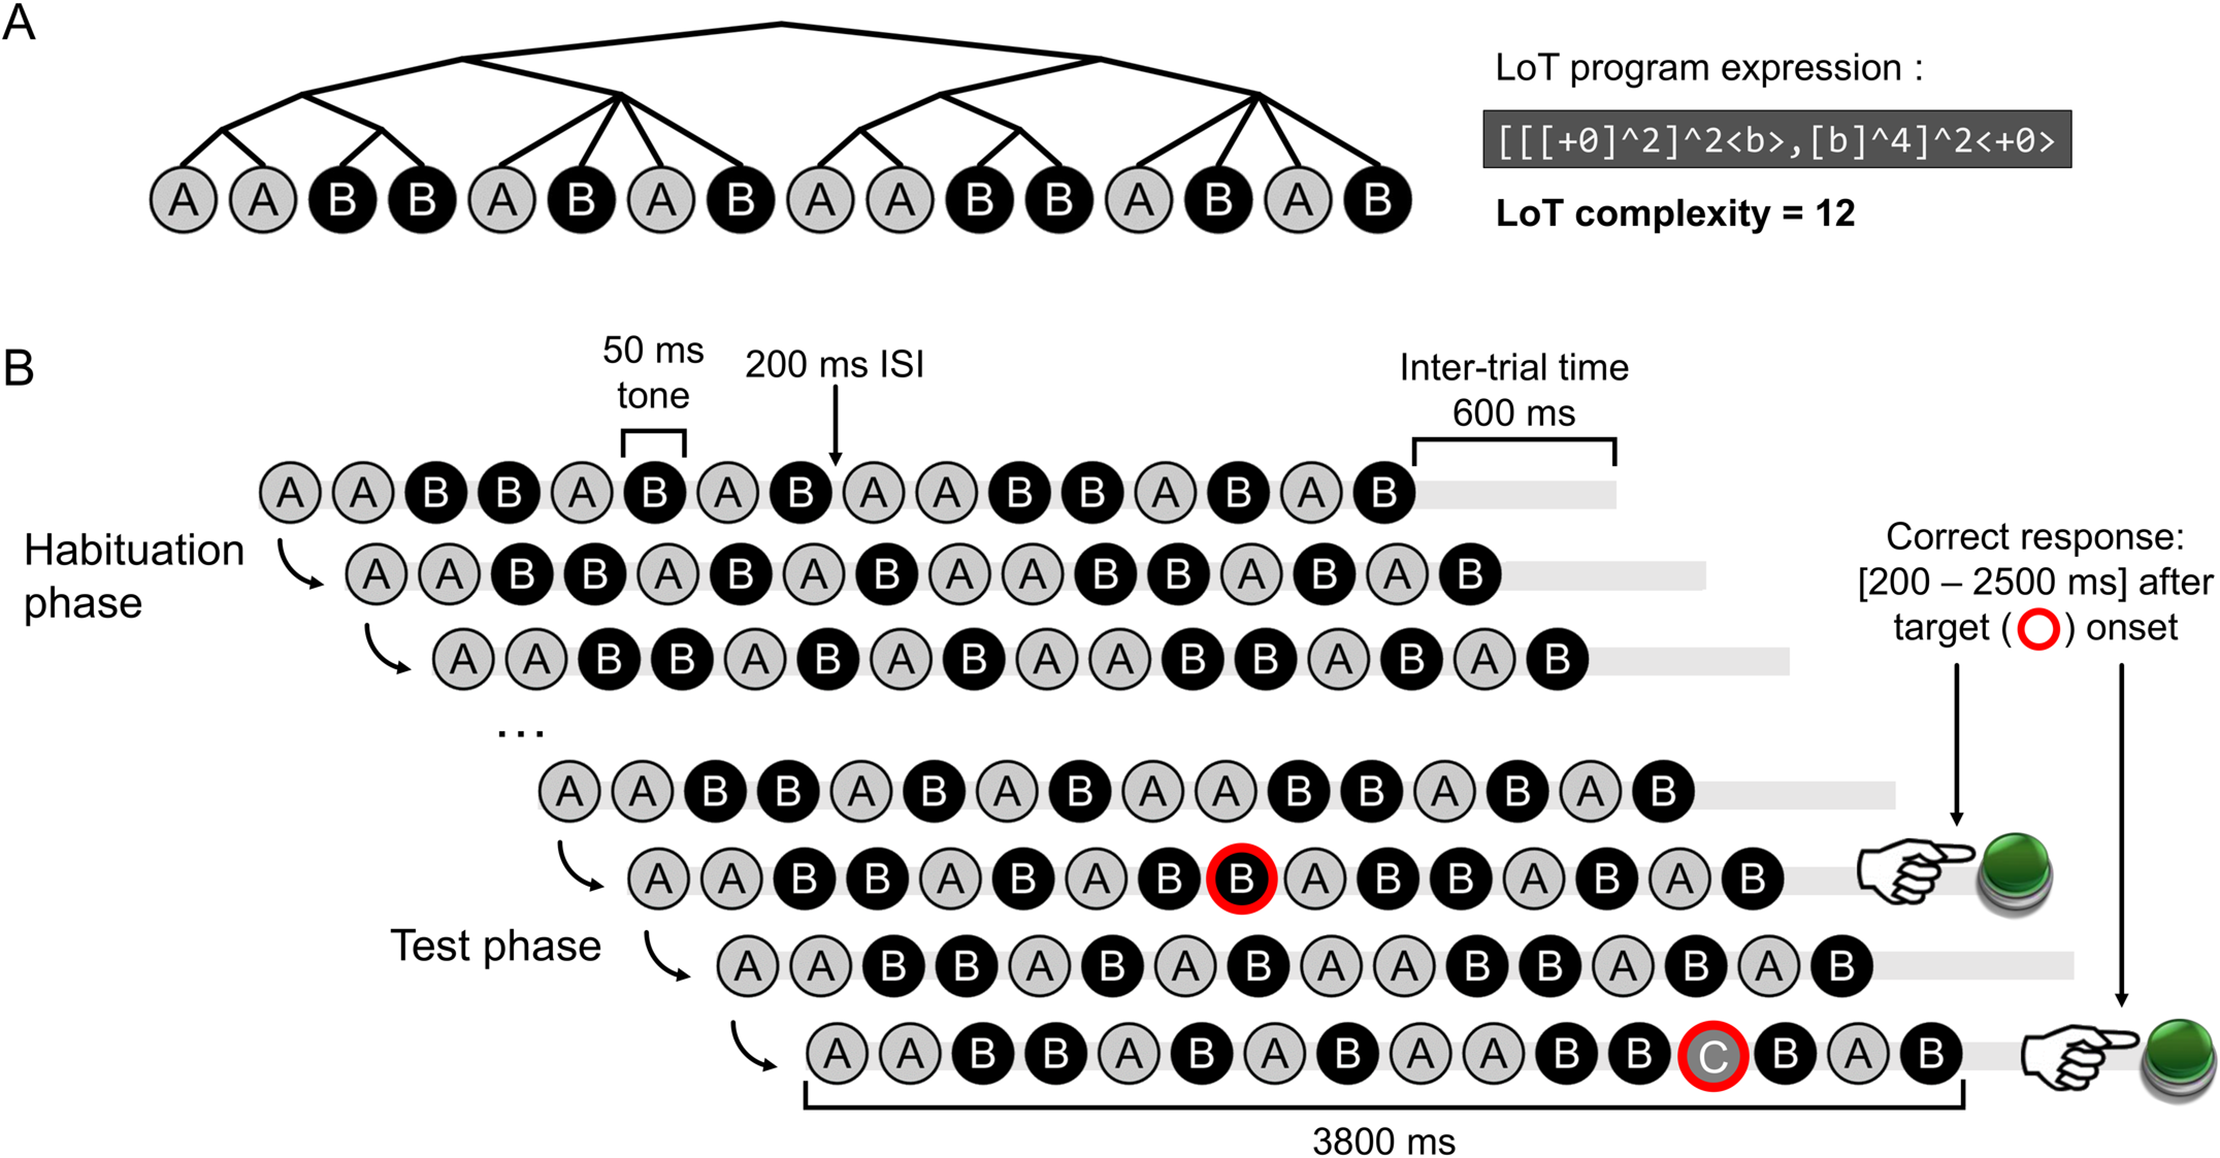
\includegraphics[scale=0.8]{journal.pcbi.1008598.g001.PNG}
   
   \centering
   %Figure 1: (A) Example of a 16-items long sequential pattern, with its shortest representation in the language of thought (i.e. LoT program expression) and the tree-structure derived from this expression (illustrating the hierarchical representation). The LoT complexity of this sequence is also indicated. (B) Experimental design of the violation detection task: a session with the sequence AABBABABAABBABAB is represented, with one example target deviant item (“A” replaced by “B”, at position 9) and one example target súper-deviant item (“C” at position 13). Deviants could occur at positions 9, 11, 13 or 15.
   
   \caption{(A) Ejemplo de un patrón de secuencia larga de 16 elementos, con su representación más corta en el LoT (es decir, la expresión del programa LoT) y la estructura de árbol derivada de esta expresión (que ilustra la representación jerárquica). También se indica la complejidad de LoT de esta secuencia. (B) Diseño experimental de la tarea de detección de violaciones: se representa una sesión con la secuencia AABBABABAABBABAB, con un ejemplo de elemento desviado objetivo (A reemplazado por B, en la posición 9) y un ejemplo de elemento súper-desviador objetivo (C en la posición 13). Las desviaciones podían ocurrir únicamente en las posiciones 9, 11, 13 o 15}
   \label{PlosBIO-F1}
\end{figure}
\sergio{la figura no está traducida}  

\begin{figure}[t!]
   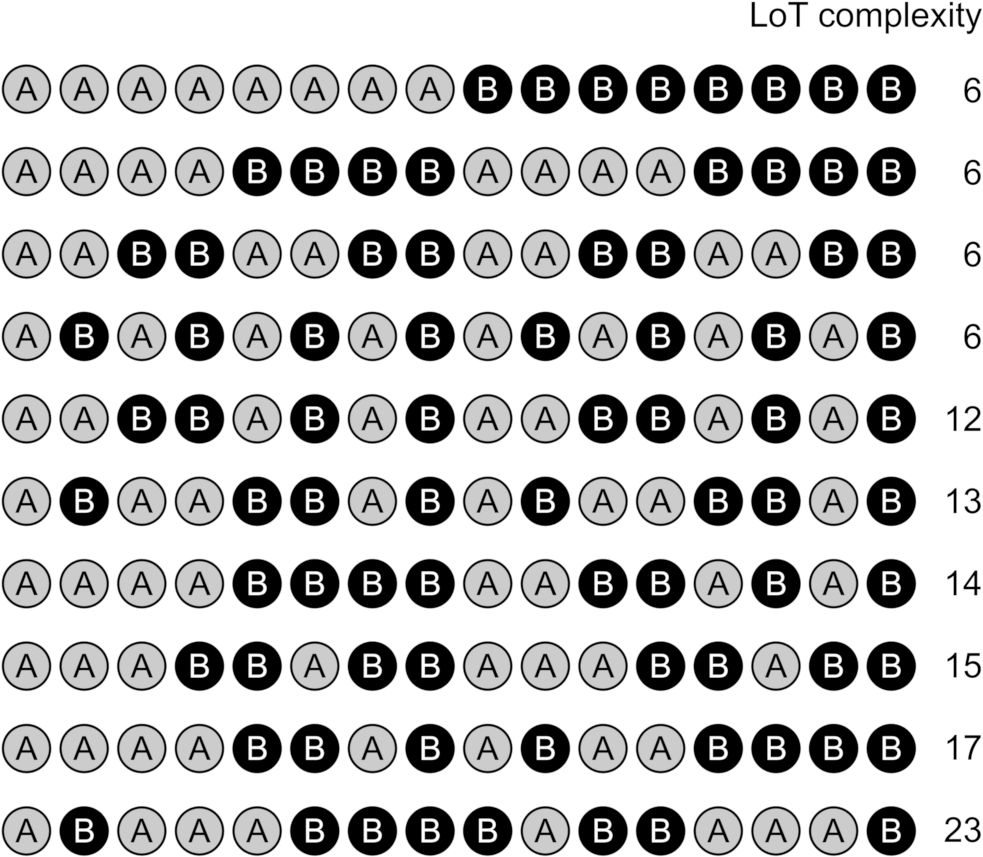
\includegraphics[scale=1]{journal.pcbi.1008598.g002.PNG}
   \centering
   %Ten 16-items long sequential patterns used in experiment 1, with their corresponding LoT complexity value.
   \caption{Diez patrones de secuencias largas de 16 elementos usados en el experimento 1, con su correspondiente valor de complejidad de LoT}
   \label{PlosBIO-F2}
\end{figure}
\sergio{la figura no está traducida}

\subsubsection*{Tarea de calificación de complejidad}

%We observed a strong positive linear relationship between average subjective complexity ratings and LoT complexity (entered as a fixed factor in the linear mixed model including participants as the random factor: t(278) = 24.6, p < .0001; Pearson correlation coefficient on the average ratings for each sequence: r = .94) (see Figure 3A). These results indicate that participants were readily able to judge whether a pattern is “more complex” than another, and that the formal language we used to compute sequence complexity is close to how individuals form such complexity judgements.

Se observó una fuerte relación lineal positiva entre la complejidad subjetiva promedio reportada y la complejidad LoT (introducida como un factor fijo en el modelo mixto lineal que incluye participantes como el factor aleatorio: $t (278) = 24.6, p < 0,0001;$ coeficiente de correlación de Pearson en las calificaciones promedio para cada secuencia: $r = .94$) \santi{unificar 0.X vs 0,X (punto vs coma)}(ver Figura~\ref{PlosBIO-F3}A). Estos resultados indican que los participantes pudieron juzgar fácilmente si un patrón es ``más complejo'' que otro, y que el lenguaje formal que usamos para calcular la complejidad de la secuencia se acerca a cómo los individuos forman tales juicios de complejidad.

\subsubsection*{Efectos de tipo de desviación y complejidad en la tarea de detección de infracciones}

%We observed a linear relationship of LoT complexity and performance in the violation detection task (using the Linear Integrated Speed-Accuracy Score, LISAS, an integrated measure of response times and error rates, see 87,88). We observed main effects of LoT complexity (t(415.0) = 18.1, p < .0001), deviant type (994 ms for sequence deviants vs. 570 ms for súper-deviants; t(414.4) = 18.9, p < .0001) and their interaction (t(414.5) = 11.7, p < .0001). Indeed, the slope of the complexity effect was significantly stronger, by an order of magnitude, for sequence deviants as opposed to súper-deviants (respectively +51 ms vs. +5 ms in simple regression, t(16) = 11.7, p < .0001; see Figure 3B, and Fig. S1 for the corresponding results using response times or miss rate instead of LISAS). Nevertheless, separate analyses revealed that LoT complexity was a strong predictor of performance for sequence deviants (t(193.0) = 15.5, p < .0001; r = .98) and also, surprisingly, for súper-deviants (t(198.5) = 4.08, p < .0001; r = .72) (Figure 3B). The latter effect on LISAS was however mainly driven by response times, since the average hit-rate for súper-deviants was high (96\%) and weakly modulated by LoT complexity (t(200.7) = 2.32, p = .022).

Observamos una relación lineal entre la complejidad LoT y el rendimiento en la tarea de detección de violaciones (utilizando la medida \textit{linear integrated speed-accuracy score} (LISAS), una medida integrada de tiempos de respuesta y tasas de error, ver~\cite{f87,f88}). Hemos observado efectos principales de complejidad LoT ($t(415.0) = 18.1, p <0,0001$), tipo de desviación (994ms para desviaciones de secuencias vs. 570ms para súper-desviaciones; $t (414.4) = 18.9, p < .0001$) y su interacción ($t(414.5) = 11. 7, p < .0001$). De hecho, la pendiente del efecto de complejidad fue significativamente más fuerte, en un orden de magnitud, para las desviaciones de secuencia en comparación con las súper-desviaciones (respectivamente +51ms frente a +5ms en la regresión lineal, $t(16) = 11.7, p <0.0001$; consultar la Figura~\ref{PlosBIO-F3}B y la Figura~\ref{PlosBIO-S1} para los resultados correspondientes utilizando el tiempo de respuesta o la tasa de errores en lugar de LISAS). Sin embargo, análisis separados revelaron que la complejidad LoT era un fuerte predictor de rendimiento para la desviación de secuencias ($t(193.0) = 15.5, p <0.0001; r = 0.98$) y también, sorprendentemente, para súper-desviaciones ($t (198.5) = 4.08, p < .0001; r = .72$) (Figura~\ref{PlosBIO-F3}B). El último efecto en LISAS, sin embargo, fue impulsado principalmente por el tiempo de respuesta, ya que la tasa de éxito promedio para súper-desviaciones fue alta (96\%) y débilmente modulada por la complejidad LoT ($t(200.7) = 2.32, p = .022$).

%The number of false alarms per sequence (which was 1.99 on average) also increased with sequence LoT complexity (t(214.4)=4.20, p < .0001; r = .74), suggesting here again that the LoT complexity was a good predictor of the quality of sequence encoding.

El número de falsas alarmas\santi{se entiende qué es una falsa alarma?} por secuencia (que era 1.99 en promedio) también aumentó con la complejidad LoT de la secuencia ($t(214.4)= 4.20, p <0.0001; r = 0.74$), lo que sugiere de nuevo que la complejidad LoT es un buen predictor de la calidad de la codificación de secuencias.

%The results of this first experiment with long binary auditory sequences (16 items) thus indicate that the formal language used to describe sequences in a compressed form, based on simple (possibly embedded) rules, is highly relevant to predict (i) how “complex” an auditory sequence is judged by adult participants after having listened to it once and (ii) how difficult it was to learn these sequences in order to detect alterations. 

Los resultados de este primer experimento con secuencias binarias auditivas largas (16 elementos) indican, por lo tanto, que el lenguaje formal utilizado para describir la secuencia en una forma comprimida, basado en reglas simples con capacidad de ser embebidas\santi{embebidas es una mala traducción de embedding. Se refiere a anidadas?}, es de gran importancia para predecir (i) cuán ``compleja'' una secuencia auditiva es juzgada por los participantes adultos después de haberla escuchado una vez y (ii) lo difícil que fue aprender estas secuencias para que puedan detectar alteraciones.

%Sequence complexity was expected to have little or no impact on the detection of súper-deviants, i.e. high or low pitch tones different from the two tones composing the binary auditory sequence. Our rationale was that such “C” tones were detectable even without any prior knowledge of sequence structure. While performance in detecting súper-deviants was much better than for sequence deviants, even for the simplest sequences, a clear relationship between LoT complexity and performance continued to be observed. We see at least two interpretations of this finding. First, there could be an increased attentional cost of having to detect violations in more complex sequences, thus placing subjects in a dual-task setting of having to simultaneously maintain a complex representation in memory and to respond to deviants. Alternatively, the effect could reflect the influence of a top-down prediction system which would use sequence structure to generate predictions of the incoming stimuli. Complex sequences would be less well predicted, and this would in turn affect the speed with which any deviant is detected. We return to this question in the General Discussion.

Se esperaba que la complejidad de la secuencia tenga poco o ningún impacto en la detección de súper-desviadaciones, (tonos altos o bajos diferentes de los dos tonos que componen la secuencia auditiva binaria). Nuestro razonamiento fue que esos tonos C eran detectables incluso sin ningún conocimiento previo de la estructura de la secuencia. Si bien el rendimiento en la detección de súper-desviaciones fue mucho mejor que para las desviaciones de secuencia, incluso para las secuencias más simples, se siguió observando una relación clara entre la complejidad LoT y el rendimiento. Vemos al menos dos interpretaciones de este hallazgo. Primero, podría haber un mayor costo de atención de tener que detectar violaciones en secuencias más complejas, colocando así a los sujetos en un entorno de una doble tarea de tener que mantener simultáneamente una representación compleja en la memoria y responder a las desviaciones. Alternativamente, el efecto podría reflejar la influencia de un sistema de predicción de arriba hacia abajo que usaría la estructura de secuencia para generar predicciones de los estímulos entrantes. Las secuencias complejas se predecirían peor y esto, a su vez, afectaría la velocidad con la que se detecta cualquier desviación. Volvemos a esta cuestión en la~\ref{chapter:BOI-GeneralDiscusion}.\santi{roto}

\subsubsection*{Efectos de sorpresa}\santi{Efectos sorpresa? EN TODO EL CAPITULO}

%Many prior experiments, using either or both behavior and brain-imaging measures, have shown that individuals constantly entertain predictions about future observations using probabilistic knowledge based on past observations (e.g. 19,20). In order to test whether task performance could be explained by a learning transition probabilities (surprise) only, or also truly implied an encoding of sequence structure, we compared a mixed model (with participants as a random effect) including fixed effects of both LoT complexity and surprise (averaged across the 4 possible positions of deviants in a given sequence) with a null model including only surprise. The effect of surprise in the null model with surprise alone) was significant (t(193.0) = 5.31, p < .0001). However, a likelihood ratio test showed that adding LoT complexity significantly improved the goodness of fit: χ²(1) = 130.9, p < .0001. Adding a “period” factor (i.e. period values were 2, 4, 8 or 16) as a third fixed effect did not improve the model fit (χ2(1) = 1.23, p = .267), confirming the prediction that the four included AnBn patterns have the same psychological complexity, and suggesting that this information is already captured by LoT complexity. Adding the interaction between surprise and LoT complexity did not improve goodness of fit either (χ2(1) = 2.50, p = .114). As reported in Table 1, the LoT complexity fixed effect was significant in the final full model (t(192.4) = 13.6, p < .0001), but not the surprise fixed effect (t(191.8) = 0.60, p = .55). The absence of a significant effect of surprise once sequence complexity is taken into account reflects the existence of a correlation between the two measures (r = –.54): biased transition probabilities in less complex sequences tending to make deviants more easily surprising. It also shows that when these two slightly colinear factors are included, LoT is more effective than surprise at describing the variance of the data.

Muchos experimentos previos, utilizando alguna o ambas medidas de comportamiento y de imagen cerebral, han demostrado que los individuos constantemente generan predicciones de futuras observaciones usando el conocimiento probabilístico basado en observaciones anteriores (por ejemplo,~\cite{f19,f20}). Para probar si el desempeño de la tarea podría explicarse sólo como un aprendizaje de la transición de probabilidad (sorpresa), o si también implicaba realmente una codificación de la estructura de la secuencia, comparamos un modelo mixto (con participantes como un efecto aleatorio) que incluye efectos fijos de complejidad LoT y sorpresa (promediada entre las 4 posibles posiciones de las desviaciones en una secuencia dada) con un modelo nulo que incluye sólo la sorpresa. El efecto de sorpresa en el modelo nulo con sorpresa sola fue significativo ($t(193.0) = 5.31, p < .0001$). Sin embargo, una prueba de razón de verosimilitud\santi{que es prueba de razón de verosimilitud?} mostró que agregar la complejidad LoT mejoraba significativamente la bondad de ajuste: $\chi^2(1) = 130.9, p < .0001$. Agregar un factor de ``período'' (los valores del período fueron 2, 4, 8 o 16) como un tercer efecto fijo no mejoró el ajuste del modelo ($\chi^2(1) = 1.23, p = .267$), lo que confirma la predicción de que los cuatro patrones $A^n B^n$\santi{deinido?} incluidos tienen la misma complejidad subjetiva, y sugiere que esta información ya está capturada por la complejidad LoT. La adición de la interacción entre la sorpresa y la complejidad LoT tampoco mejoró la bondad del ajuste ($\chi^2(1) = 2.50, p = . 114$). Como se informa en la Tabla~\ref{PlosBIO-T1}, el efecto fijo de la complejidad LoT fue significativo en el modelo completo final ($t(192.4) = 13.6, p < .0001$), pero no el efecto fijo de la sorpresa ($t (191.8) = 0.60, p = .55$). La ausencia de un efecto de sorpresa significativo una vez que se tiene en cuenta la complejidad de la secuencia refleja la existencia de una correlación entre las dos medidas ($r = -.54$): probabilidades de transición sesgadas en secuencias menos complejas tienden a hacer que las desviaciones sean más fácilmente sorprendentes. También muestra que cuando se incluyen dos factores con una pequeña colinealidad, LoT es más eficaz que la sorpresa en la descripción de la varianza de los datos.

%As our choice of attributing an arbitrary padding value (0.01) to deviant transitions events with zero probability when computing surprise may have biased the results, we recomputed the LISAS and average surprise while excluding all such trials (i.e. all deviant positions in the (AB)8 pattern, 3 out of 4 deviant positions in the A8B8 pattern). Here again, a likelihood ratio test showed that the goodness of fit increased significantly when adding LoT complexity to a null model containing only surprise (χ²(1) = 116.3, p < .0001). However, both complexity (t(165.5) = 12.9, p < .0001) and surprise (t(165.8) = 3.82, p < .0001) were significant with this subset of the data.

Como nuestra elección de atribuir valor arbitrario de relleno (0.01) a los eventos de transición de desviaciones con probabilidad cero al calcular la sorpresa puede haber sesgado los resultados, recomputamos la medida LISAS y la media de la sorpresa excluyendo todos esos ensayos (es decir, todas las posiciones de desviación en el patrón $(AB)^8$ y 3 de 4 posiciones de desviación en el patrón $A^8 B^8$).\santi{está definido este exponente?} Aquí nuevamente, una prueba de razón de verosimilitud mostró que la calidad del ajuste aumentó significativamente cuando se agregó la complejidad LoT a un modelo nulo que sólo contenía sorpresa ($\chi^2(1) = 116.3, p < .0001$). Sin embargo, tanto la complejidad ($t (165.5) = 12.9, p < .0001$) como la sorpresa (t ($165.8) = 3.82, p < .0001$) fueron significativas con este subconjunto de datos. \sergio{entender efecto de relleno explicado}\santi{si, por favor ;)}

%In conclusion, the strong complexity effects observed here indicated that participants used some form of compression of information to encode the sequence and perform the task over and above simply learning statistical trends. Although no instruction was given in that sense, this strategy may be needed in order to deal with a difficult, memory-demanding task. Indeed, at the maximum level of complexity used, performance in violation detection was very low (the violation detection rate dropped to 41% for sequence deviants).

En conclusión, los fuertes efectos de complejidad observados indicaron que los participantes usan alguna forma de compresión de la información para codificar la secuencia y realizar la tarea más allá de simplemente aprender tendencias estadísticas de los elementos. Aunque no se dio ninguna instrucción en ese sentido, esta estrategia puede ser necesaria para hacer frente a una tarea difícil que exige memoria. De hecho, en el nivel máximo de complejidad utilizado, el rendimiento en la detección de violaciones fue muy bajo (la tasa de detección de violaciones se redujo al 41\% para las desviaciones de secuencias).

%In the subsequent experiments, we asked whether similar complexity effects emerged in the same paradigm but with shorter sequences. That is, when the sequence can be more easily encoded and stored “as a whole”, without necessarily requiring a re-encoding in a more abstract, compressed form. In these less demanding conditions, it can be expected that the spontaneous encoding of transitions probabilities between items will play a more important role in the detection of violations.

En los experimentos posteriores, nos preguntamos si los efectos de complejidad similares pueden ser vistos en el mismo paradigma, pero con secuencias más cortas. Es decir, cuando la secuencia se puede codificar y almacenar más fácilmente ``en su conjunto'', sin que se requiera necesariamente una recodificación en una forma más abstracta o comprimido.\santi{revisar redaccion de Es decir,...} En estas condiciones menos exigentes, se puede esperar que la codificación espontánea de las probabilidades de transición entre elementos juegue un papel más importante en la detección de violaciones.

\begin{figure}[t!]
   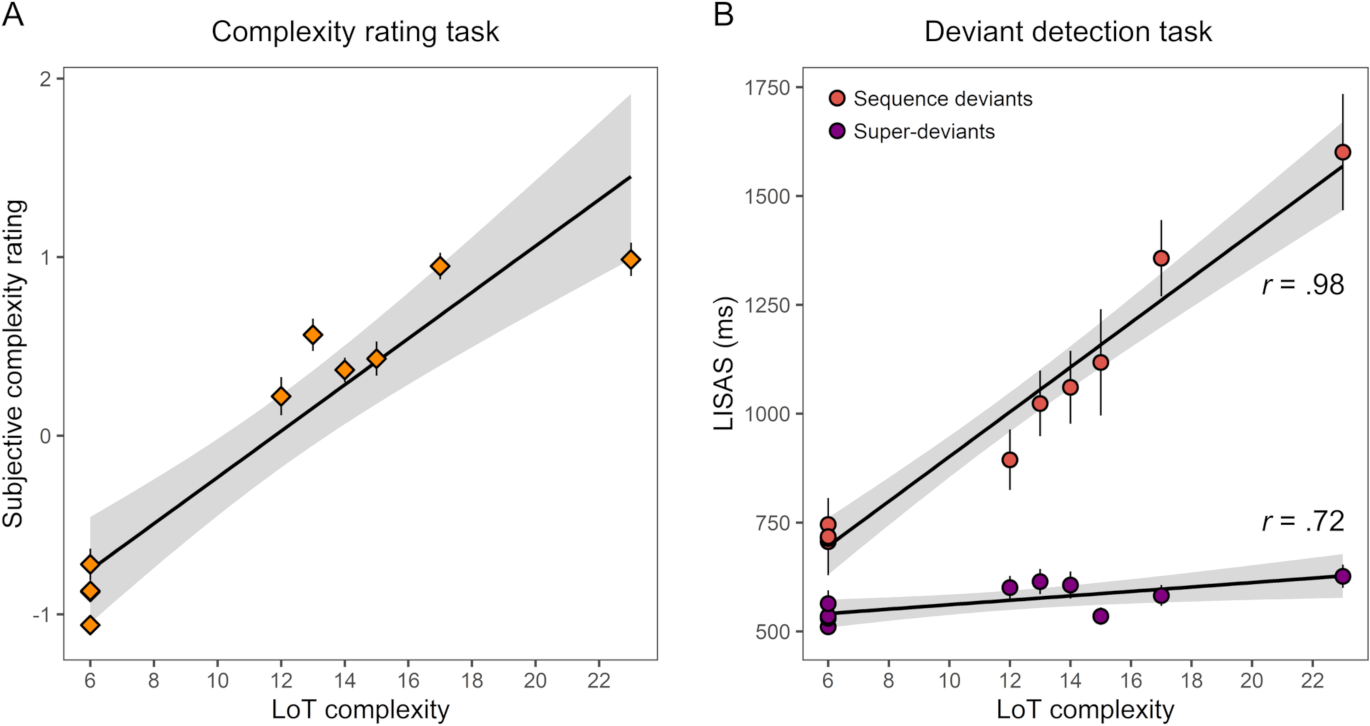
\includegraphics[scale=1]{journal.pcbi.1008598.g003.PNG}
   \centering
   %Linear relationship between LoT complexity and subjective and objective measures obtained in experiment 1 with ten 16-items long auditory sequences (with 95% confidence intervals bands in gray). The Pearson correlation coefficient (r) is indicated. Each marker represents the group-average for a given sequence. Error bars represent SEM across participants. (A) LoT complexity vs. subjective complexity ratings. (B) LoT complexity vs. performance in the violation detection task (Linear Integrated Speed-Accuracy Score), for sequence deviants and súper-deviants.
   \caption{Relación lineal entre la complejidad LoT y las medidas subjetivas y objetivas obtenidas en el experimento 1 con diez secuencias auditivas largas de 16 elementos (intervalos de confianza del 95\% en gris). El coeficiente de correlación de Pearson ($r$) aparece indicado. Cada marcador representa el promedio del grupo para una determinada secuencia. Las barras de error representan el s.e.m. entre los participantes. (A) Clasificación de complejidad LoT frente a complejidad subjetiva. (B) Complejidad LoT frente a rendimiento en la tarea de detección de violaciones (medida integrada de tiempos de respuesta y tasas de error, LISAS), para desviaciones de secuencia y súper-desviaciones.}
   \label{PlosBIO-F3}
\end{figure}
\sergio{la figura no está traducida}

\santi{que es pag en la tabla?}
\begin{table}[]
\centering
\begin{tabular}{lccccc}
\multicolumn{6}{l}{\textbf{Experimento 1} (secuencias de 16 elementos, excluyendo súper-desviados)}                          \\ \hline
\textit{Predictores}     & \textit{Estimados}  & \textit{Std. Error} & \textit{Valor t}   & \textit{IC del 95\%} & \textit{pag}       \\ \hline
(Interceptar)         & 356,90        & 80,51        & 4.43         & 199,5 - 514,3    & \textbf{\textless{}.0001} \\
Complejidad          & 52.15        & 3,84         & 13.60        & 44,6 - 59,7     & \textbf{\textless{}.0001} \\
Sorpresa           & 6,77         & 11.31        & 0,60         & -15,4 - 28,9     &.55            \\ \hline
\multicolumn{1}{c}{}     & \multicolumn{1}{l}{} &           &           &           &              \\
\multicolumn{6}{l}{\textbf{Experimento 2} (secuencias de 12 elementos, excluyendo súper-desviados)}                          \\ \hline
\textit{Predictores}     & \textit{Estimados}  & \textit{Std. Error} & \textit{Valor t}   & \textit{IC del 95\%} & \textit{pag}       \\ \hline
(Interceptar)         & 852,38        & 124,91        & 6,82         & 608,5 - 1096,2    & \textbf{\textless{}.0001} \\
Complejidad          & 24,21        & 6.29         & 3,85         & 11,9 - 36,5     & \textbf{\textless{}.0002} \\
Sorpresa           & -43,13        & 21.06        & -2.05        & -84,4 - -1,9     & \textbf{\textless{}.05}  \\ \hline
\textbf{}           & \multicolumn{1}{l}{} & \multicolumn{1}{l}{} & \multicolumn{1}{l}{} & \multicolumn{1}{l}{} & \multicolumn{1}{l}{}   \\
\multicolumn{6}{l}{\textbf{Experimento 3} (secuencias de 8 elementos)}                                        \\ \hline
\textit{Predictores}     & \textit{Estimados}  & \textit{Std. Error} & \textit{Valor t}   & \textit{IC del 95\%} & \textit{pag}       \\ \hline
(Interceptar)         & 852.40        & 73,39        & 11,62        & 707,8 - 997     & \textbf{\textless{}.0001} \\
Complejidad          & 10,75        & 3,49         & 3,08         & 3,9 - 17,6      & \textbf{\textless{}.003} \\
Sorpresa           & -32,37        & 5.60         & -5,78        & -43,3 - -21,4    & \textbf{\textless{}.0001} \\ \hline
\multicolumn{1}{c}{\textbf{}} & \multicolumn{1}{l}{} & \multicolumn{1}{l}{} & \multicolumn{1}{l}{} & \multicolumn{1}{l}{} & \multicolumn{1}{l}{}   \\
\multicolumn{6}{l}{\textbf{Experimento 4} (secuencias de 6 elementos, secuencia 'AAAAAA' excluida)}                          \\ \hline
\textit{Predictores}     & \textit{Estimados}  & \textit{Std. Error} & \textit{Valor t}   & \textit{IC del 95\%} & \textit{pag}       \\ \hline
(Interceptar)         & 751,6        & 47,5         & 15,8         & 658,8 - 844,5    & \textbf{\textless{}.0001} \\
Complejidad          & 1.4         & 4.4         & 0,3         & -7,2 - 9,9      &.75            \\
Sorpresa           & -15,3        & 3.8         & -4,1         & -22,7 - -7,9     & \textbf{\textless{}.0001} \\ \hline
\multicolumn{1}{c}{\textbf{}} & \multicolumn{1}{l}{} & \multicolumn{1}{l}{} & \multicolumn{1}{l}{} & \multicolumn{1}{l}{} & \multicolumn{1}{l}{}   \\
\multicolumn{6}{l}{\textbf{Experimento 5} (secuencias de 8 ítems, auditivo y visual)}                                 \\ \hline
\textit{Predictores}     & \textit{Estimados}  & \textit{Std. Error} & \textit{Valor t}   & \textit{IC del 95\%} & \textit{pag}       \\ \hline
(Interceptar)         & 645,1        & 92,2         & 7.0         & 464,4 - 825,9    & \textbf{\textless{}.0001} \\
Complejidad          & 25,2         & 25,2         & 4.4         & 14 - 36,4      & \textbf{\textless{}.0001} \\
Sorpresa           & -36,7        & 8.1         & -4,5         & -52,5 - -20,8    & \textbf{\textless{}.0001} \\
Modalidad (visual)      & 337,0        & 337,0        & 14,2         & 290,7 - 383,3    & \textbf{\textless{}.0001} \\ \hline
\end{tabular}
\caption{Efectos fijos en los modelos lineales mixtos, separados para cada experimento}
\label{PlosBIO-T1}
\end{table}

\subsection{Experimento 2: secuencias auditivas con 12 elementos}
\label{ploscomp-results-exp2}

%In order to test whether the previous results could be replicated with shorter sequences, in experiment 2, the same tasks and procedure were used (with a different group of participants), this time using twelve sequences of twelve items (spanning a large range of complexities, see Figure 4).

Para probar si los resultados anteriores podían replicarse con secuencias más cortas, en el experimento 2, se utilizaron las mismas tareas y el mismo procedimiento (con un grupo diferente de participantes), pero esta vez usando doce secuencias de doce elementos (que abarcan una amplia gama de complejidades, vea la Figura~\ref{PlosBIO-F4}).

\begin{figure}[t!]
   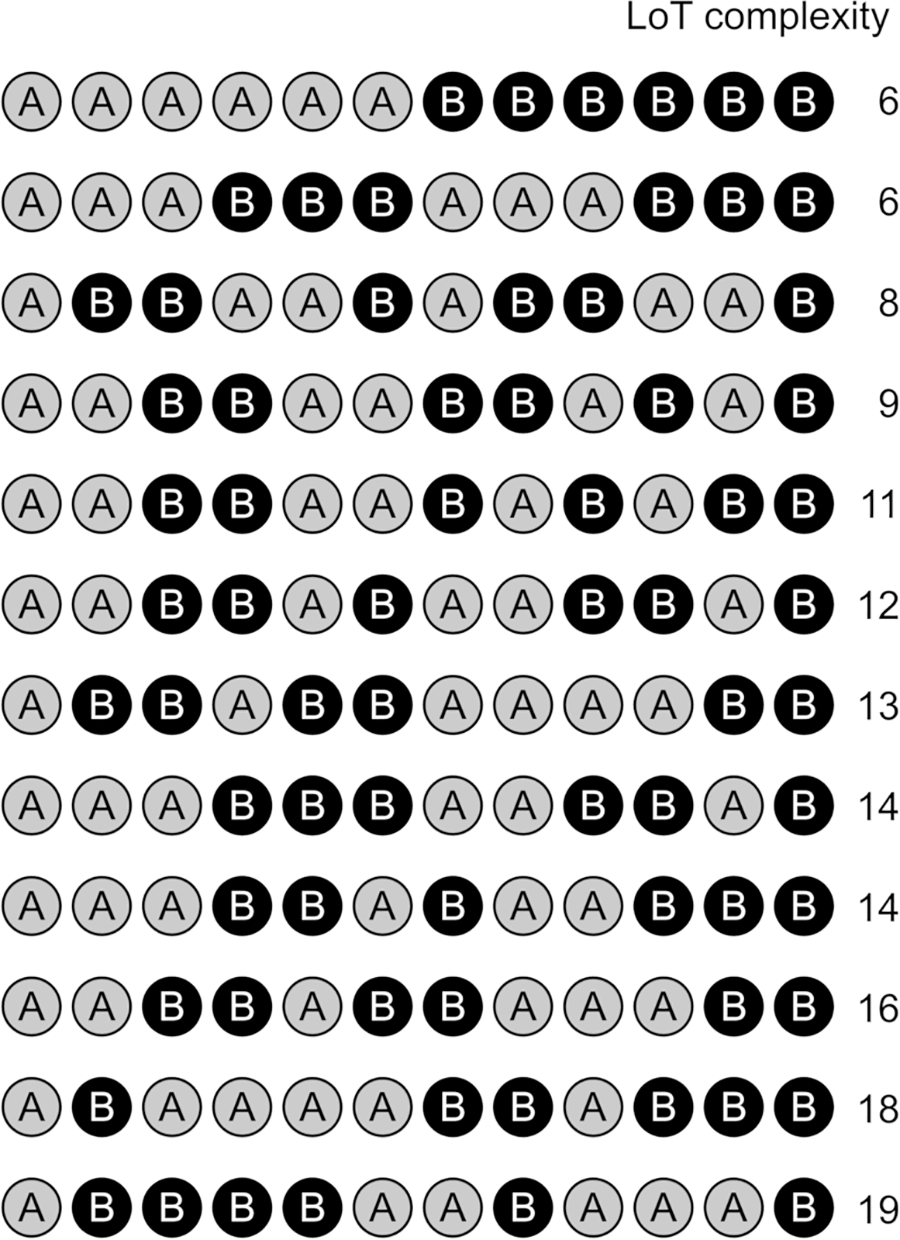
\includegraphics[scale=1]{journal.pcbi.1008598.g004.PNG}
   \centering
   %Twelve 12-item sequences used in experiment 2, with their corresponding LoT complexity value (in bits).
   \caption{Doce secuencias de 12 elementos utilizadas en el experimento 2, con su correspondiente valor de complejidad LoT (en bits)}
   \label{PlosBIO-F4}
\end{figure}
\sergio{la figura no está traducida}

\subsubsection*{Tarea de calificación de complejidad}

%A positive linear relationship was found between subjective complexity ratings and LoT complexity (t(238) = 6.81 p < .0001, r = .61). The correlation of the average score per sequence with LoT complexity was however less strong than what was observed in the previous experiment with 16-items long sequences (r = .61, see Figure 5A). Subjective complexity was clearly underestimated for one specific sequence (ABBAABABBAAB, predicted complexity of 8), which is confirmed by an inspection of the residuals of the regression (residual 1.99 SD above average for this sequence).

Se encontró una relación lineal positiva entre los reportes de complejidad subjetiva y la complejidad LoT ($t(238) = 6.81 p < .0001, r = .61$). La correlación de la complejidad subjetiva media por secuencia con la complejidad LoT era, sin embargo, menos fuerte que lo observado en el experimento anterior con 16 secuencias largas de 16 elementos ($r = .61$, ver Figura~\ref{PlosBIO-F4}A). La complejidad subjetiva estuvo claramente subestimada para una secuencia específica (ABBAABABBAAB, con una complejidad predicha de 8), lo cual se confirma con una inspección de los residuos de la regresión (residual 1.99 SD por encima del promedio para esta secuencia).

%Deviant type and complexity effects in the violation detection task
\subsubsection*{Tipos de desviaciones y efectos de la complejidad en la tarea de detección de violaciones}

%Regarding the violation detection task, main effects of LoT complexity (t(431.1) = 6.43, p < .0001) and deviant type (1078 ms for sequence deviants vs. 545 ms for súper-deviants; t(431.0) = 19.3, p < .0001) were observed, as well as their interaction (t(431.1) = 3.48, p < .001). The slope of the complexity effect appeared indeed slightly stronger for sequence deviants as opposed to súper-deviants, although the comparison did not reach significance when using simple linear regressions with averaged LISAS per sequence (slopes of respectively +30 ms vs. +7 ms, t(20) = 1.87, p = .077; see Figure 5B, and Fig. S2 for the corresponding results with RTs and miss rates instead of LISAS). Separated analyses revealed that the effect of LoT complexity was significant in analyses restricted to either sequence deviants (t(205.1) = 5.78, p < .0001; r = .63), or súper-deviants (t(208.0) = 2.88, p = .005; r = .59) only. The number of false alarms per sequence (3.88 on average) was also significantly predicted by the LoT complexity of the sequence (t(208.0) = 3.50, p < .001; r = .56).

\santi{chequear redaccion de Con respecto a...}Con respecto a la tarea de detección de violaciones, los principales efectos de la complejidad LoT ($t (431.1) = 6.43, p < .0001$) y el tipo de desviación (1078 ms para desviaciones de secuencia vs 545 ms para súper-desviaciones; $t (431.0) = 19.3, p < .0001$), así como su interacción ($t (431.1) = 3.48, p < .001$). La pendiente del efecto de complejidad apareció de hecho ligeramente más fuerte para las desviaciones de secuencia en comparación con las súper-desviaciones, aunque la comparación no fue significativa cuando se usaron regresiones lineales simples con LISAS promediado por secuencia (pendientes de +30 ms frente a +7 ms, respectivamente, $t (20) = 1.87, p = .077$; consultar la Figura~\ref{PlosBIO-F5}B y la Figura~\ref{PlosBIO-S2} para obtener los resultados correspondientes con tiempo de respuesta y tasas de error en lugar de LISAS). Los análisis separados revelaron que el efecto de la complejidad LoT fue significativo en los análisis restringidos a secuencias con desviaciones ($t (205.1) = 5.78, p < .0001; r = .63$), o súper-desviaciones ($t (208.0) = 2.88, p = .005; r = .59$) solamente. El número de falsas alarmas por secuencia (3.88 en promedio) también fue predicho significativamente por la complejidad LoT de la secuencia ($t (208,0) = 3,50, p < .001; r = .56$).

%As in the complexity rating task, although the overall correlation was high, a noticeable deviation between predicted complexity and observed performance was present for some of the sequences. In fact, the correlation profiles observed in the Figure 5A and 5B suggest that the psychological complexity of the pattern, as indexed by subjective rating or violation detection task performance, might have been, for some sequences, consistently overestimated or underestimated by the LoT across both tasks (the largest residual in the regression with the sequence deviants, 1.50 SD above average, corresponded to the same sequence identified by complexity ratings: ABBAABABBAAB). To further test this idea, we computed the correlation between the residuals of both linear regressions. The correlation was significant (t(10) = 4.02; p = .003), indicating that even after regressing out the effect of LoT complexity, the data from both experiments remained correlated with each other, and thus that, although the proposed LoT is a good predictor, it does not fully account for all details of the psychological complexity of patterns. One attempt to address the limitations of the language, by proposing a modification of it, is reported in the Further analysis section.

Al igual que en la tarea de calificación de complejidad, aunque la correlación general fue alta, hubo una desviación notable entre la complejidad predicha y el rendimiento observado para algunas de las secuencias. De hecho, los perfiles de correlación observados en la Figura~\ref{PlosBIO-F5}A y la Figura~\ref{PlosBIO-F5}B sugieren que la complejidad psicológica del patrón, según lo indexado por la calificación subjetiva o el desempeño de la tarea de detección de violaciones, podría haber sido para algunas secuencias constantemente sobrestimado o subestimado por el LoT en ambas tareas (el residuo más grande en la regresión con las desviaciones de secuencia, 1.50 SD por encima del promedio, correspondió a la misma secuencia identificada por la clasificación de complejidad subjetiva: ABBAABABBAAB). Para probar más esta idea, calculamos la correlación entre los residuos de ambas regresiones lineales. La correlación fue significativa ($t (10) = 4.02; p = .003$), lo que indica que --incluso después de hacer una regresión del efecto de la complejidad LoT-- los datos de ambos experimentos permanecieron correlacionados entre sí y, por lo tanto, aunque el LoT propuesto es un buen predictor, no explica por completo todos los detalles de la complejidad psicológica de los patrones. Un intento de abordar las limitaciones del lenguaje, proponiendo una modificación, se informa en la sección~\ref{PlosBIO-AnalisisAdiocional}.\santi{roto}

\begin{figure}[t!]
   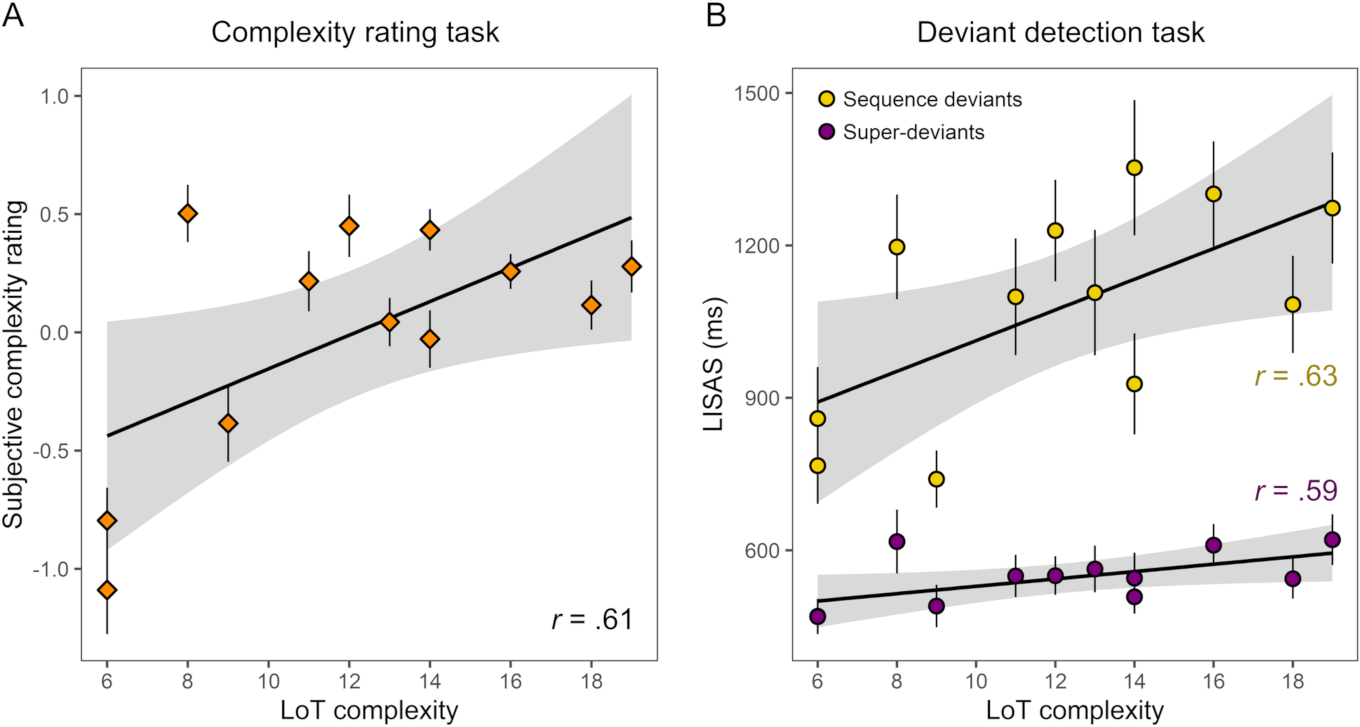
\includegraphics[scale=1]{journal.pcbi.1008598.g005.PNG}
   \centering
   %Linear relationship between LoT complexity and scores obtained in the two tasks of experiment 2 with 12-item auditory sequences (with 95% confidence intervals bands in gray). Same format as Figure 3.
   \caption{Relación lineal entre la complejidad LoT y las puntuaciones obtenidas en las dos tareas del experimento 2 con secuencias auditivas de 12 elementos (con bandas de intervalos de confianza del 95\% en gris). Mismo formato que la Figura~\ref{PlosBIO-F3}}
   \label{PlosBIO-F5}
\end{figure}
\sergio{la figura no está traducida}

\subsubsection*{Efectos de sorpresa}
%A comparison of mixed models (with participants as a random effect) showed that, compared to a null model including surprise as the sole predictor (null model; in which the main predictor was significant: t(205.0) = 4.67, p < .0001), a model additionally including LoT complexity (full model) fitted the data better (likelihood ratio test : χ²(1) = 14.4, p < .001). Both fixed effects were significant in the full model: LoT complexity (t(204.1) = 3.85, p < .0001), as well as surprise (t(204.0) = 2.05, p = .042) (see Table 1). Although we observed, contrary in the previous experiment, an effect of statistical learning (indexed by the level of surprise of deviant items), it was only barely statistically significant.

Una comparación de modelos mixtos (con participantes como el efecto aleatorio) \santi{redacción EN TODO EL CAPITULO: con participantes como el efecto aleatorio vs con participantes como un efecto aleatorio vs con participantes como efecto aleatorio} mostró que, en comparación con un modelo nulo que incluye la sorpresa como único predictor (modelo nulo en el que el predictor principal fue significativo: $t (205,0) = 4,67, p <0,0001$), un modelo que incluye adicionalmente la complejidad LoT (modelo completo) explica mejor los datos (prueba de razón de verosimilitud: $\chi^2(1) = 14.4, p < .001$). Ambos efectos fijos fueron significativos en el modelo completo: complejidad LoT ($t (204.1) = 3.85, p < .0001$), así como la sorpresa ($t (204.0) = 2.05, p= .042$) (ver Tabla~\ref{PlosBIO-T1}). \santi{redacción: Aunque hemos observado...}Aunque hemos observado, al contrario que en el experimento anterior, un efecto de aprendizaje estadístico (indexado por el nivel de la sorpresa del elemento desviado), que era sólo apenas estadísticamente significativo.

\subsection{Experimento 3 y 4: secuencias auditivas con 6 u 8 elementos}

%Results of experiments 1 and 2 showed that our sequence complexity metric was well correlated with behavior, suggesting that our formal language provided a good approximation of the internal language of thought that humans use to encode a sequence in memory a compressed from. These results were however obtained with a restricted set of sequences, which were long enough to promote hierarchical representations based on the repetition and alternation operations, and to probe a large range of complexity values. The main objective of experiments 3 (with 35 8-items long sequences, see Fig. S3) and 4 (with 32 6-items long sequences, see Fig. S4) was to test whether the effect of complexity observed in the first two experiments could be generalized to a larger set of shorter sequences, where we could examine more gradual variations in complexity. Given that human working memory is thought to store and maintain 4 to 7 items without compression, or with a minimal chunking process (25,29), we expected the predictive power of our language to be reduced compared with previous experiments with longer sequences, while the effects of transition probabilities would increase. The same violation detection paradigm was used. No subjective complexity ratings were collected (given the larger number of individual sequences compared to the previous experiments). 

Los resultados de los experimentos 1 y 2 mostraron que nuestra métrica de complejidad de secuencia se correlacionaba bien con el comportamiento, lo que sugiere que nuestro lenguaje formal proporcionó una buena aproximación del lenguaje interno del pensamiento que los humanos usan para codificar una secuencia comprimida en la memoria. Sin embargo, estos resultados se obtuvieron con un conjunto restringido de secuencias, que eran lo suficientemente largas para promover representaciones jerárquicas basadas en las operaciones de repetición y alternancia, y para probar una amplia gama de valores de complejidad. El objetivo principal del experimento 3 (con 35 secuencias largas de 8 elementos,\santi{no se entiende lo de largas de 8 o largas de 6} ver Figura~\ref{PlosBIO-S3}) y del experimento 4 (con 32 secuencias largas de 6 elementos, ver Figura~\ref{PlosBIO-S4}) fue probar si el efecto de la complejidad observado en los dos primeros experimento podría ser generalizados a un conjunto más amplio de secuencias más cortas,\santi{aclarar a qué se refiere con cortas y largas} en donde podamos examinar variaciones más graduales de la complejidad. Dado que la memoria de trabajo humana está pensada para almacenar y mantener de 4 a 7 elementos sin compresión, o con un proceso de agrupamiento mínimo~\cite{f25,f29}, esperamos que le poder predictivo de nuestro LoT se reduzca en comparación con los experimentos anteriores realizados con secuencias más largas, mientras que los efectos de las transiciones de probabilidad aumenten. Utilizamos en estos experimentos el mismo paradigma de detección de violaciones. No se recopilaron calificaciones de complejidad subjetiva (dado el mayor número de secuencias individuales en comparación con los experimentos anteriores).

%Here again, we tested (using mixed models) whether surprise suffices to explain the variance in performance or if a significant proportion of variance remained yet to be explained by sequence complexity (all models included participants as a random effect). In experiment 3 (8-items sequences, N = 35), goodness of fit improved when LoT complexity was included in the model (χ²(1) = 9.47, p = .002). Both fixed effects were significant in the full model: LoT complexity (t(1042.0) = 3.08, p = .002; see Figure 6A, and Fig. S5), as well as surprise (t(1042.0) = 5.78, p < .0001) (see Table 1). Note that the surprise fixed effect was already highly significant in the null model (t(1043.0) = 8.72, p < .0001).

Una vez más, hemos testeado (utilizando modelos mixtos) si es suficiente la sorpresa para explicar la variación en el rendimiento o si una proporción significativa de la varianza se mantuvo aún para ser explicada por la complejidad de la secuencia (todos los modelos incluyen los participantes como efecto aleatorio). En el experimento 3 (secuencias de 8 elementos, N = 35), la calidad del ajuste mejoró cuando se incluyó la complejidad LoT en el modelo ($\chi^2(1) = 9.47, p= .002$). Ambos efectos fijos fueron significativos en el modelo completo: complejidad LoT ($t (1042.0) = 3.08, p <= .002$; ver Figura~\ref{PlosBIO-F6}A y Figura~\ref{PlosBIO-S5}), así como la sorpresa ($t (1042.0) = 5.78, p < .0001$) (ver Tabla~\ref{PlosBIO-T1}). Tener en cuenta que el efecto fijo de la sorpresa\santi{efecto de la sorpresa vs efecto sorpresa EN TODO EL CAPITULO} ya era muy significativo en el modelo nulo ($t (1043.0) = 8.72, p < .0001$).

%Similarly, in experiment 4 (6-items sequences, N = 32), goodness of fit improved when LoT complexity was included in the surprise-only null model (χ²(1) = 6.20, p = .013) with both fixed effects significant in the full model (LoT complexity: t(649.00) = 2.49, p = .013; see Figure 6B, and Fig. S6), and surprise (t(649.0) = 5.48, p < .0001). The surprise fixed effect was here again already highly significant in the null model (t(650.0) = 6.78, p < .0001). However, one sequence appeared as an outlier in this experiment, with an average LISAS 3.9 SD below the average of all sequences (i.e. indicating a much better performance): the AAAAAA sequence. In this case, performing the task requires no sequence learning, but merely remembering the identity of the A sound, and violation detection is therefore similar to a classic oddball paradigm. When this sequence was removed from the dataset (it was also excluded from further analyses), the inclusion of the complexity fixed factor did no longer improved model goodness of fit (χ²(1) = 0.10, p = .752). Indeed, the LoT complexity fixed effect was not significant in the full model (t(628.0) = 0.32, p = .752), as opposed to the surprise fixed effect (t(628.0) = 4.07, p < .0001) (see Table 1). No improvement in model fit was found when including the interaction between complexity and surprise (χ²(1) = 0.08 in experiment 3, χ²(1) = 0.34 in experiment 4).

Del mismo modo, en el experimento 4 (secuencias de 6 elementos, N = 32), la calidad del ajuste mejoró cuando la complejidad LoT se incluyó en el modelo nulo con la sorpresa como único factor ($\chi^2(1) = 6.20, p= .013$) con ambos efectos fijos significativos en el modelo completo (complejidad LoT: $t (649.00) = 2.49, p= .013$; ver Figura~\ref{PlosBIO-F6}B y Figura~\ref{PlosBIO-S6}) y sorpresa ($t (649.0) = 5.4 8, p < .0001$). El efecto fijo de la sorpresa fue ya aquí otra vez altamente significativo en el modelo nulo ($t (650.0) = 6.78, p < .0001$). Sin embargo, una secuencia apareció como un valor atípico en este experimento, con un LISAS 3,9 SD promedio por debajo del promedio de todas las secuencias (es decir, indicando un rendimiento mucho mejor): la secuencia AAAAAA. En este caso, realizar la tarea no requiere un aprendizaje de secuencia, sino simplemente recordar la identidad del sonido A, y la detección de la violación es, por lo tanto, similar a un paradigma clásico de bichos raros\santi{se dice bichos raros en castellano?} (\textit{oddball}). Cuando esta secuencia se eliminó del conjunto de datos (también se excluyó de análisis posteriores), la inclusión del factor fijo de complejidad ya no mejoró la bondad de ajuste del modelo ($\chi^2 (1) = 0.10, p = .752$). De hecho, el efecto fijo de la complejidad LoT no fue significativo en el modelo completo ($t (628.0) = 0.32, p = .752$), a diferencia del efecto fijo de la sorpresa ($t (628.0) = 4.07, p < .0001$) (ver Tabla~\ref{PlosBIO-T1}). No se encontró ninguna mejora en el ajuste del modelo al incluir la interacción entre complejidad y sorpresa ($\chi^2(1) = 0.08$ en el experimento 3, $\chi^2(1) = 0.34$ en el experimento 4).

%Beside the effect of complexity, the strong effect of surprise in both experiments indicates that participants were quicker and more likely to detect a deviant when it violated statistical regularities characterizing the auditory sequence being repeatedly played. This is consistent with the idea that humans spontaneously encode the probabilities associated with events and react to surprising events depending on their level of predictability (19,21).

Además del efecto de la complejidad, el fuerte efecto de la sorpresa en ambos experimentos indica que los participantes fueron más rápidos y más propensos a detectar un desviado\santi{desvío?} cuando violaba las regularidades estadísticas que caracterizan la secuencia auditiva que se reproduce repetidamente. Esto es consistente con la idea de que el ser humano codifica de manera espontánea las probabilidades asociadas con eventos y reacciona a los eventos sorprendentes en función de su nivel de previsibilidad~\cite{f19,f22}.

%The number of false alarms was low in the present experiments (0.91 per sequence on average in experiment 3, 0.60 in experiment 4). It was slightly related to sequence complexity in experiment 3 t(1048) = 2.19, p = .029) but not in experiment 4 t(650.0) = 0.29, p = .77).

El número de falsas alarmas fue bajo en los presentes experimentos (0.91 por secuencia en promedio en el experimento 3, 0.60 en el experimento 4). Estuvo levemente relacionado con la complejidad de la secuencia en el experimento 3 ($t (1048) = 2.19, p= .029$) pero no en el experimento 4 ($t (650.0) = 0. 29, p = . 77$).

%Compared to the previous experiment with lengths 12 and 16, it was expected here, with sequences of 8 or 6 items, that the effect of LoT complexity would be mitigated, since those auditory sequences may become short enough to be stored in working memory as a simple chain (note that the range of LoT complexity values was also smaller). The correlation of performance with LoT complexity was in fact still present with 8-items sequences (at a similar level as in experiment 2) but disappeared with 6-items sequences. This is in line with the assumption that complexity is tightly linked with the idea of compressibility in memory, and suggests that such a compression strategy, whether it is simple chunking or involves a hierarchical representation, is more likely to be involved when the number of items to store in working memory exceeds the typical working memory span (16,89). However, rather than a clear threshold above which complexity would become predictive of performance, the estimates of the LoT complexity effect across the four experiments (in the mixed models taking into account surprise) reveal a gradient: with stronger effects of complexity for longer sequences (respectively +1.4 ms, +10.8 ms, +24.2 ms, and +52.2 ms, for the experiments with length 6, 8, 12 and 16 respectively; see Table 1). The effect of surprise seemed to follow an inverse trend, with insignificant or marginal effects in long sequences (experiments 1 and 2) and highly significant effects in short sequences (experiments 3 and 4). To test this idea, the data from experiments 1-4 (excluding súper-deviants) were combined in a single mixed model including the three fixed factors of LoT complexity, surprise and length (as a continuous predictor), as well as the three two-way interactions (with participants as the random factor). An ANOVA on the mixed model revealed main effects of LoT complexity (F(1, 2336.4) = 48.0, p < .0001) and surprise (F(1, 2334.1) = 4.91, p = .027). The main effect of sequence length was marginally significant (F(1, 96.6) = 3.08, p = .082). As expected, a strong interaction between LoT complexity and length was present (F(1, 2347.5) = 63.3, p < .0001), indicating a stronger effect of complexity when sequence length increased. The estimated slopes for the LoT complexity effect indeed increased with each sequence length (+15.5 ms, +46.0 ms, +107.1 ms, and +168.1 ms, for length 6, 8, 12 and 16, respectively). The interaction between length and surprise was not significant (F(1, 2330.0) = 1.19, p = .276). However, the estimated slopes for the surprise effect followed our initial observation: they decreased with each sequence length (-15.6 ms, -12.0 ms, -4.9 ms, and +2.2 ms).

En comparación con los experimentos anteriores con longitud 12 y 16, se esperaba aquí, con secuencias de 8 o 6 elementos, que el efecto de la complejidad LoT se mitigaría, ya que esas secuencias auditivas pueden volverse lo suficientemente cortas como para ser almacenadas en la memoria de trabajo como una cadena simple (tener en cuenta que el rango de valores de complejidad LoT también fue menor). La correlación de rendimiento con la complejidad LoT se mantuvo de hecho\santi{redaccción: se mantuvo de hecho...} todavía presente en las secuencias de 8 elementos (a un nivel similar como en el experimento 2) pero desaparece con las secuencias de 6 elementos. Esto está en línea con la suposición de que la complejidad está estrechamente vinculada con la idea de compresibilidad en la memoria, y sugiere de que dicha estrategia de compresión (ya sea un simple agrupamiento o que implique una representación jerárquica) es más probable que tenga un rol cuando el número de los elementos que se almacenan en la memoria de trabajo exceden el intervalo de memoria de trabajo típico~\cite{f16,f89}. Sin embargo, en lugar de un umbral claro por encima del cual la complejidad se convertiría en predictiva para el rendimiento, las estimaciones del efecto de complejidad LoT en los cuatro experimentos (en los modelos mixtos teniendo en cuenta la sorpresa) revelan un gradiente: con efectos de complejidad más fuertes para secuencias más largas (+1,4 ms, +10,8 ms, +24,2 ms y +52,2 ms, para los experimentos con longitud 6, 8, 12 y 16 respectivamente; consultar la Tabla~\ref{PlosBIO-T1}). El efecto de sorpresa parecía seguir una tendencia inversa, con efectos no significativos o marginales en secuencias largas (experimentos 1 y 2) y efectos altamente significativos en secuencias cortas (experimentos 3 y 4). Para probar esta idea, los datos de los experimentos 1 al 4 (excluyendo súper-desviaciones) fueron combinados en un único modelo mixto que incluye los tres factores fijos: complejidad LoT, sorpresa y longitud (como un predictor continuo), así como la tres interacciones bidireccionales (con los participantes como factor aleatorio). Un ANOVA en el modelo mixto reveló efectos principales de la complejidad LoT ($F (1, 2336.4) = 48.0, p <0,0001$) y sorpresa ($F (1, 2334.1) = 4.91, p = .027$). El factor principal de longitud de la secuencia fue marginalmente significativo ($F (1, 96.6) = 3.08, p = 0.082$). Como era de esperar, estuvo presente una fuerte interacción entre la complejidad LoT y la longitud ($F (1, 2347.5) = 63.3, p < .0001$), lo que indica un efecto más fuerte de complejidad cuando la longitud de la secuencia aumenta. Las pendientes estimadas para el efecto de complejidad LoT aumentaron de hecho con cada longitud de secuencia (+15,5 ms, +46,0 ms, +107,1 ms y +168,1 ms, para las longitudes 6, 8, 12 y 16, respectivamente). La interacción entre la longitud y la sorpresa no era significativa ($F (1, 2330.0) = 1.19, p = .276$). Sin embargo, las pendientes estimadas para el efecto sorpresa siguieron nuestra observación inicial: disminuyeron con cada longitud de secuencia ($-15,6$ms, $-12,0$ms, $-4,9$ms y $+ 2,2$ms).

\begin{figure}[t!]
   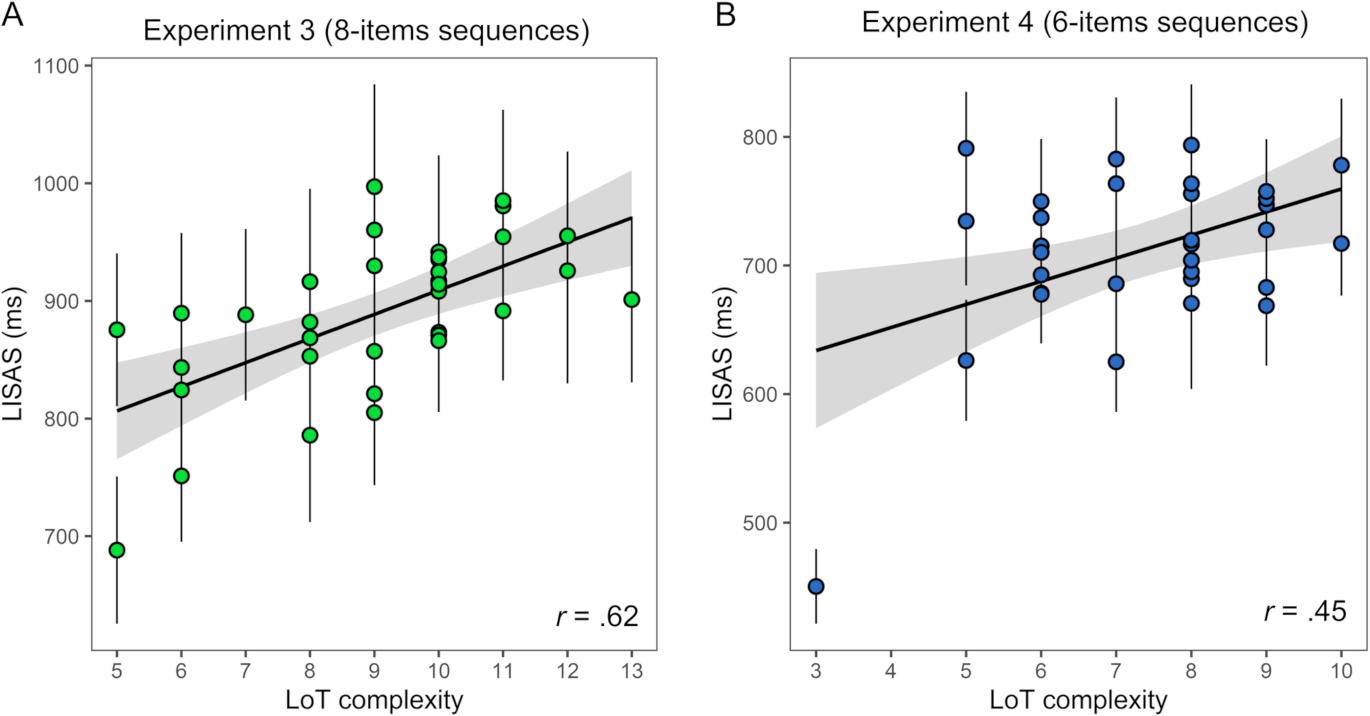
\includegraphics[scale=1]{journal.pcbi.1008598.g006.PNG}
   \centering
   %Linear relationship between LoT complexity and violation detection task performance (LISAS) in: (A) experiment 3 (8-items sequences) and (B) experiment 4 (6-items sequences).
   \caption{Relación lineal entre la complejidad LoT y el desempeño de la tarea de detección de violaciones (LISAS) en: (A) Experimento 3 (secuencias de 8 elementos) y (B) Experimento 4 (secuencias de 6 elementos)}
   \label{PlosBIO-F6}
\end{figure}
\sergio{la figura no está traducida}

\subsection{Experimento 5: secuencias auditivas y visuales}

%The observation of a LoT complexity effect on sequences of length 8 and higher is consistent with our initial claim that individuals spontaneously apply simple rules (mainly based on nested repetitions) in order to recode auditory sequences in a compressed abstract form in memory. It may be argued, however, that rather than being abstract and universal, some of these effects may reflect the great ability of our auditory system to manipulate and find regularities in acoustic stimuli (90); whether it is in spoken language or in music listening. In experiment 5, we wished to replicate the findings of previous experiment and extend them to the visual modality. Although we expected a reduced performance, given that audition is generally superior to vision in the processing of temporal information (91), we still predicted a correlation of performance with our complexity metric, since our language was originally designed for a visual paradigm (58) and relies on abstract mental operations rather than on specific acoustic coding mechanisms. Twelve sequences of 8 items (see Fig. S7), allowing to use a sufficient number of trials while still expecting clear complexity effects, were presented to a group of participants in both a visual and in an auditory form (in different experimental blocks), using the same violation detection paradigm. Due to constraints in the perception of repeated visual stimuli, stimulus onset asynchrony was lengthened to 400 ms in both auditory and visual sessions, resulting in a sequence duration of 3000 ms (compared to 1800 ms in experiment 2).

La observación de un efecto de la complejidad LoT en secuencias de longitud 8 y superior es consistente con nuestro planteo inicial de que los individuos espontáneamente aplican reglas simples (basadas principalmente en repeticiones anidados) con el fin de recodificar secuencias auditivas en una forma abstracta más comprimida en la memoria. Sin embargo, se puede argumentar que --en lugar de ser abstractos y universales-- algunos de estos efectos pueden reflejar la gran capacidad de nuestro sistema auditivo para manipular y encontrar regularidades en los estímulos acústicos~\cite{f90}; ya sea en el lenguaje hablado o escuchando música. En el experimento 5, deseamos replicar los hallazgos del experimento anterior y extenderlos a una modalidad visual. A pesar de que esperábamos un rendimiento reducido (dado que la audición es generalmente superior a la visión en el procesamiento de información temporal~\cite{f91}) todavía esperamos encontrar una correlación del rendimiento con nuestra métrica de complejidad, ya que nuestro lenguaje fue diseñado originalmente para un paradigma visual~\cite{amalric2017language} y se basa en operaciones mentales abstractas más que en mecanismos de codificación acústica específicos. Se presentaron a un grupo de participantes doce secuencias de 8 elementos (ver Figura~\ref{PlosBIO-S7}) tanto en forma visual como auditiva (en diferentes bloques experimentales), utilizando el mismo paradigma de detección de violaciones. Debido a las limitaciones en la percepción de estímulos visuales repetidos, la asincronía inicio\santi{redacción} de estímulo se alargó a $400$ms en ambas sesiones (auditivas y visuales), lo que resulta en una duración de la secuencia de $3000$ms (en comparación con $1800$ms en el experimento 2).

\subsubsection*{Efectos de complejidad y modalidad}

%To assess the impact of LoT complexity and modality on performance, we first estimated a mixed model including complexity and modality as fixed factors and participants as a random factor. Effects of LoT complexity (t(486.0) = 3.08, p = .003), modality (average LISAS of 1110 ms in visual blocks vs. 780 ms in auditory blocks; t(486.0) = 14.1, p < .0001) and their interaction (t(486.0) = 3.19, p = .002) were significant. The slope of the complexity effect was steeper in the visual than in the auditory modality (+54 ms vs. +22 ms, t(486) = 3.19; see Figure 7, and Fig. S8). Separate analyses indicated that LoT complexity was a strong predictor of performance for visual sequences (t(233.0) = 6.82, p < .0001; r = .76), and also for auditory sequences (t(237.0) = 3.76, p < .001; r = .63).

\widesanti{este párrafo que sigue tenía muchos errores. Revisarlo bien, incluyendo números (lo los pasé a modo math)}
Para evaluar el impacto de la complejidad y la modalidad de LoT en el rendimiento, primero estimamos un modelo mixto que incluye la complejidad y la modalidad como factores fijos y los participantes como un factor aleatorio. Efectos de la complejidad de LoT ($t (486.0) = 3.08$, $p = .003$), modalidad (LISAS promedio de 1110 ms en bloques visuales vs 780 ms en bloques auditivos; $t (486.0) = 14.1$, $p < .0001$) y su interacción ($t (486.0) = 3.19$, $p< = 0,002$) fueron significativas. La pendiente del efecto de complejidad fue más pronunciada en la modalidad visual que en la auditiva ($+54$ ms frente a $+22$ ms, $t (486) = 3,19$; ver Figura 7 y Figura S8).\santi{falta link a figuras} Análisis separados indicaron que LoT complejidad era un fuerte predictor de rendimiento para secuencias visuales ($t (233.0) = 6,82$, $p <0,0001$; $r. = 76$), y también para las secuencias auditivas ($t (237,0) = 3,76$, $p < . 001$;$ r = .63$).

%Note that, although the effects appeared stronger in the visual modality, the average performance in the visual and the auditory modality were highly correlated (r = .85, p < .0001). This suggests a common, cross-modal mechanism underlying the observed differences in performance between sequences. It can however be acknowledged, here again, that differences in performance across sequences are not entirely explained by complexity: residuals of linear regressions with LoT complexity in the visual and in the auditory modality (using average LISAS per sequence) were correlated (r = .73, t(13) = 3.92; p = .002).

Nótese que, aunque los efectos parecían más fuertes en la modalidad visual, el desempeño promedio en la modalidad visual y auditiva estuvieron altamente correlacionados ($r = .85, p < .0001$). Esto sugiere un mecanismo común entre las modalidades que subyace a las diferencias observadas en el rendimiento entre secuencias. Sin embargo, se puede reconocer nuevamente que las diferencias en el rendimiento entre secuencias no se explican completamente por la complejidad: los residuos de regresiones lineales con la complejidad LoT en la modalidad visual y en la modalidad auditiva (usando LISAS promedio por secuencia) estuvieron correlacionados ($r = .73, t (13) = 3.92; p = .002$).

%The number of false alarms per sequence was related to the task modality (mean number of FA: 0.58 in auditory blocks; 1.16 in visual blocks; difference between modalities: t(487.0) = 5.73, p < .0001) but not to sequence LoT complexity (t(487.0) = 0.08, p = .935).

El número de falsas alarmas por secuencia se relacionó con la modalidad de la tarea (número medio de FA : 0.58 en bloques auditivos; 1.16 en bloques visuales; diferencia entre modalidades: $t (487.0) = 5.73, p <0.0001$) pero no con la complejidad LoT ($t(487.0) = 0.08, p = .935$).

\begin{figure}[t!]
   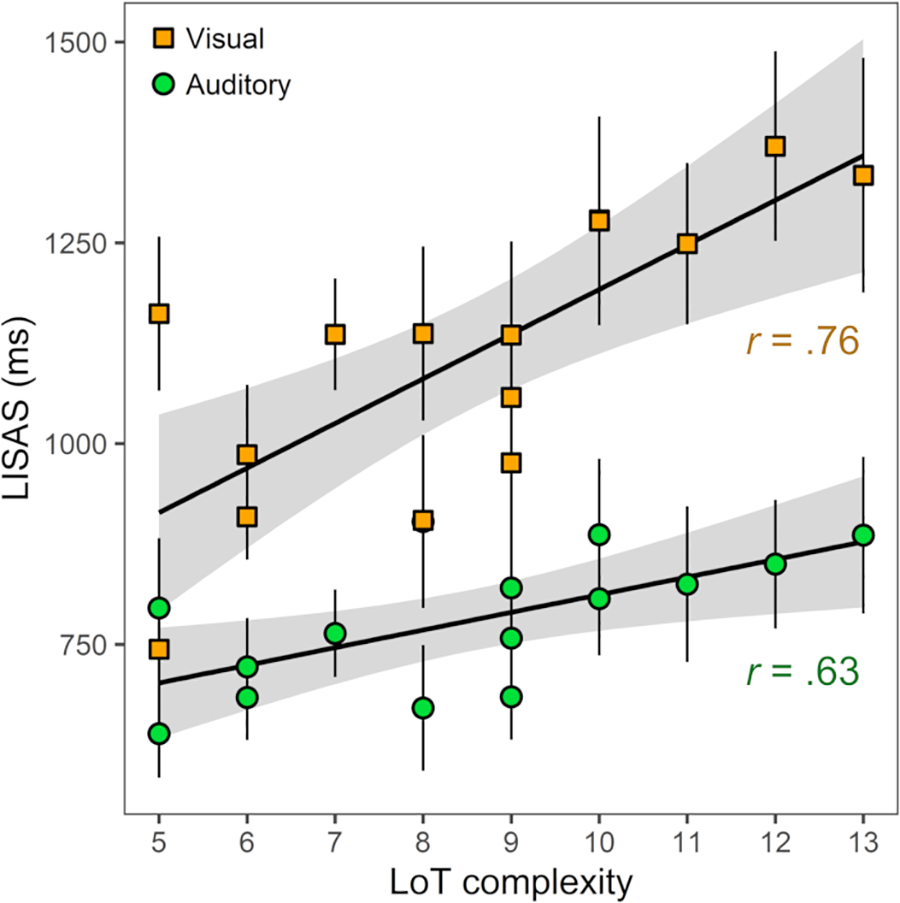
\includegraphics[scale=1]{journal.pcbi.1008598.g007.PNG}
   \centering
   % Linear relationship between LoT complexity and violation detection task performance (LISAS) for each modality in experiment 5 (8-items auditory and visual sequences).
   \caption{Relación lineal entre complejidad LoT y rendimiento en tareas de detección de violación (LISAS) para cada modalidad en experimento 5 (secuencias auditivas y visuales de 8 elementos)}
   \label{PlosBIO-F7}
\end{figure}
\sergio{la figura no está traducida}

\subsubsection*{Efectos de sorpresa}

%As in previous experiments, a surprise effect was also observed in both modalities when considered independently: deviants inducing rare transitions were more easily and quickly detected than frequent ones (effect of surprise in a mixed model with auditory trials only: t(237.0) = 3.87, p < .001; r = –.65; with visual trials only: t(233.0) = 6.79, p < .0001; r = –.78). This effect suggests that a common, or at least similar, mechanism is at play in the encoding of statistical regularities characterizing the sequences in both the visual and the auditory modality. 

Como en los experimentos anteriores, también se observó un efecto sorpresa en ambas modalidades cuando se consideraron de forma independiente: las súper-desviaciones que inducían transiciones raras se detectaban más fácil y rápidamente que las relacionadas a elementos frecuentes (efecto de sorpresa en un modelo mixto con pruebas auditivas solamente: $t(237.0) = 3.87, p < .001; r =-.65$; solo con pruebas visuales: $t (233.0) = 6.79, p < .0001; r = –.78$). Este efecto sugiere que un mecanismo común, o al menos similar, está en juego en la codificación de regularidades estadísticas que caracterizan las secuencias tanto en la modalidad visual como en la auditiva.

%In order to test whether evidence for sequence compression could still be observed after the surprise effect was taken into account, we performed a comparison of mixed effects models. The null model included the surprise predictor, the modality as a categorical predictor and subject identity as random factor. It was compared against a full model including the same predictors, with addition of the LoT complexity. This comparison was highly significant (χ²(1) = 19.0, p < .0001), indicating that goodness of fit improved when LoT complexity was added to the model. All three fixed effects were significant in the full model (LoT complexity: t(486.0) = 4.39, p < .0001; surprise: t(486.0) = 4.54, p < .0001; modality: t(486.0) = 14.2, p < .0001, see Table 1).

Para probar si aún se podía observar evidencia de compresión de secuencia después de que se tuvo en cuenta el efecto sorpresa, realizamos una comparación de modelos de efectos mixtos. El modelo nulo incluyó el predictor de la sorpresa, la modalidad como predictor de categoría y la identidad del sujeto como factor aleatorio. Se comparó con un modelo completo que incluía los mismos predictores, con la adición de la complejidad LoT. Esta comparación fue altamente significativa ($\chi^2 (1) = 19.0, p < .0001$), lo que indica que el ajuste mejoró cuando se agregó la complejidad LoT al modelo. Los tres efectos fijos fueron significativos en el modelo completo (complejidad LoT: $t (486.0) = 4.39, p < .0001$; sorpresa: $t (486.0) = 4.54, p < .0001$; modalidad: $t (486.0) = 14.2, p <0,0001$, ver Tabla~\ref{PlosBIO-T1}).

%Overall, the results obtained in the visual modality are very similar to those obtained in the auditory modality in the same and in previous experiments. We however observed here stronger effects of both LoT complexity and surprise. It should be noted that the overall difficulty of the task increased in the visual modality (as indicated by higher average miss rates per sequence; 22\% vs. 11\%, t(14) = 7.49, p < .0001; and longer average response times per sequence; 831 ms vs. 645 ms, t(14) = 10.5, p < .0001). 8-items visual sequences may have been more difficult to encode than 8-items auditory sequences, due to the known superiority of the auditory processing system in the processing of temporal sequences and rhythms (90,92). This increased encoding difficulty in the visual domain may have in turn lead to an increased need for the “mental sequence compression” mechanism that our language of thought aims to describe.

En general, los resultados obtenidos en la modalidad visual son muy similares a los obtenidos en la modalidad auditiva en el mismo experimento y en los anteriores. Sin embargo, observamos aquí efectos más fuertes tanto de la complejidad LoT como de la sorpresa. Hay que señalar que la dificultad general de la tarea aumenta en la modalidad visual (como se indica por el aumento promedio de las tasas de error por secuencia; $22\%$ vs. $11 \%$, $t (14) = 7.49, p <0.0001$; y del tiempo medio de respuesta por secuencia; 831ms frente a 645ms, $t(14) = 10.5, p <0.0001$). Las secuencias visuales de 8 elementos pueden haber sido más difíciles de codificar que las secuencias auditivas de 8 elementos, debido a la superioridad conocida del sistema auditivo para el procesamiento de secuencias temporales y ritmos~\cite{f90,f92}. Esta mayor dificultad de codificación en el dominio visual puede, a su vez, llevar a una mayor necesidad de utilizar el mecanismo de ``compresión de la secuencia mental'' que nuestro LoT pretende describir.

%The present experiment also extends the results of experiment 3 by using a slower presentation rate. Indeed, although the participants in experiment 5 appeared to respond faster (in the auditory blocks) than those from experiment 3, the same relationship with complexity was found (correlation of performance with LoT complexity of.62 and.63 respectively). It suggests that the effect of complexity is robust across sequence durations (as expected given than LoT complexity is based on abstract sequence patterns). More importantly, the fact that a similar complexity effect was observed irrespective of the modality is consistent with the idea of “language of thought” used to compress sequential information at an abstract, symbolic level. Such an assumption has already been supported by results from Yildirim and Jacobs (93), who showed cross-modal transfer of sequence knowledge: learning to categorize visual sequences facilitated the categorization of auditory sequences and vice versa. In fact, the language we used here was initially designed to represent visually presented, geometrical patterns (58). The present results thus confirm that the present language of thought can account for sequence representations in various modalities, presentation contexts and sequence lengths.

El presente experimento extiende también los resultados del experimento 3 utilizando una tasa de presentación más lenta. De hecho, aunque los participantes del experimento 5 parecían responder más rápido (en los bloques auditivos) que los del experimento 3, se encontró la misma relación con la complejidad LoT (correlación de rendimiento con complejidad LoT de $0,62$ y $0,63$, respectivamente). Esto sugiere que el efecto de la complejidad es robusto a través de la duración de las secuencias (como se esperaba, dado que la complejidad LoT se basa en patrones de secuencias abstractos). Más importante aún, el hecho de que se observó un efecto de complejidad similar independientemente de la modalidad es consistente con la idea de un ``lenguaje de pensamiento'' (LoT)\santi{no tiene sentido esta aclaración acá. Revisar si no hay otras} utilizado para comprimir información secuencial a un nivel simbólico abstracto. Tal suposición se apoya también en los resultados de Yildirim y Jacobs~\cite{yildirim2015learning}, que mostraron efectos de transferencia de aprendizaje entre modalidades de las secuencias: aprender a categorizar secuencias visuales facilitó la categorización de secuencias auditivas y viceversa. De hecho, el lenguaje que usamos aquí fue inicialmente diseñado para representar patrones geométricos presentados de manera visual~\cite{amalric2017language}. Los presentes resultados confirman así que el lenguaje actual del pensamiento puede dar cuenta de las representaciones de secuencia en diversas modalidades, contextos de presentación y longitudes de secuencias.

\subsection{Análisis adicional: comparación con otras medidas de complejidad de secuencias}

%The complexity, or “compressibility”, of a sequence can be assessed in several ways, and various measures have been previously proposed in the psychological literature (e.g. 17,30,34,41,44,95–98). In this last section, we examined how our LoT complexity value compares to six other measures, which we list below, in predicting task performance over different sequence lengths.

La complejidad, o la ``compresibilidad'', de una secuencia se puede evaluar de varias formas, y varias medidas se han propuesto incluso previamente en la literatura psicológica~\cite{f17,f30,f34,f41,f44,f95,f96,f97,f98}. \santi{cita rota}En esta sección, examinamos cómo nuestro valor de complejidad LoT se compara con otras seis medidas para predecir el desempeño de la tarea en diferentes secuencias longitudes. Estas medidas fueron las siguientes:

%Chunk complexity: following the observation that the number of chunks (or runs) is correlated to performance in sequence encoding tasks (e.g. 34), we here define chunk complexity using the formula proposed by Mathy & Feldman (16), which they showed to correlate with performance in the encoding of series of digits:, where K is the number of chunks and Li the length of the i-th run. Note that contrary to Mathy & Feldman (16), whose sequences where composed of digits and chunks defined based on constant (positive or negative) increments from one digit to the next (e.g. “1234”, “7531”), we here simply define chunks as consecutive repetitions of the same item, e.g. the sequence “AAABAA” has a 3 chunks, and a chunk complexity of log2(4) + log2(2) + log2(3).

\paragraph{Complejidad de fragmentos.} Siguiendo la observación que el número de fragmentos (o trazas) se correlaciona con el desempeño en tareas de codificación de secuencias~\cite{f34}, definimos la complejidad de fragmentos utilizando la fórmula propuesta por Mathy \& Feldman~\cite{f34}, la cual mostraron que se correlaciona con el rendimiento en la codificación de series de dígitos. 
$$
\text{complejidad de fragmentos} = \sum_{i = 1}^{K} \log_2(1+L_i) 
$$
donde $K$ es el número de fragmentos y $L_i$ la longitud de la i-ésima traza. Se debe tener en cuenta que --al contrario que en~\cite{f34}, cuyas secuencias estaban compuestas de dígitos y los fragmentos definidos en incrementos constantes (positivos o negativos) de un dígito respecto del siguiente (por ejemplo, ``1234'', ``7531'' son ambos un sólo fragmento o traza)-- aquí simplemente definimos los fragmentos como repeticiones consecutivas del mismo elemento. Por ejemplo, la secuencia ``AAABAA'' tiene 3 fragmentos, y una complejidad de fragmentos = $\log_2(4) + \log_2(2) + \log_2(3)$.

%Entropy is a measure of information that quantifies the uncertainty of a distribution. Here, we compute the Shannon entropy of the probability of pairs of items, (AA, AB, BA, BB), in order to capture the effect of order-1 transition probabilities (85). Given that the probability of a given pair is defined as, H is computed as follow:
%H = ...
%We used the convention that 0 × log2(0) = 0 when null probabilities occurred.

\paragraph{Entropía ($H$).} Es una medida de información que cuantifica la incertidumbre de una distribución. Aquí calculamos la entropía de Shannon para la probabilidad de pares de elementos (AA, AB, BA, BB), para capturar el efecto de las probabilidades de transición de un paso~\cite{f85}.\santi{orden 1?} Dado que la probabilidad de un determinado par se define como $P(X,Y) = P(X) P(Y \mid X)$, $H$ se calcula de la siguiente manera:

\begin{align*}
H =& - [ 
     P(A) P(A \mid A) (\log_2 P(A) + \log_2 P(A\mid A)) \\
   & +P(A) P(B \mid A) (\log_2 P(A) + \log_2 P(B\mid A)) \\
   & +P(B) P(A \mid B) (\log_2 P(B) + \log_2 P(A\mid B)) \\
   & +P(B) P(B \mid B) (\log_2 P(B) + \log_2 P(B\mid B)) 
     ] 
\end{align*}
usamos la convención que $0 * \log_2(0) = 0$ cuando la probabilidad es nula.

%Lempel-Ziv complexity is derived from the popular lossless data compression algorithm, the Lempel-Ziv (LZ) algorithm (98). Briefly, the LZ algorithm works by scanning the sequence from left to right and adding to a vocabulary each new substring it has never encountered before. LZ complexity is the number of substrings in this vocabulary once the scan is complete. Beyond the field of computer data compression, LZ complexity has been used in various domains, for instance, to measure the complexity of rhythmic patterns in music (61), to account for the complexity of human (99) and mouse behaviors (100), to explain the existence of universal properties within all natural languages (101), or to measure the complexity of input-output mappings found in various domains of science and engineering (102,103). 

%The number of subsymmetries is the number of symmetric sub-sequences of any length within a sequence. For instance, the sequence AABBAB has two symmetric sub-sequences of length 2 (AA and BB), one of length 3 (BAB), and one of length 4 (ABBA), for a total of four subsymmetries. This measure was proposed by Alexander and Carey (94) and shown to be negatively correlated to performance in perception and production tasks with visual and auditory patterns (94,104). 

\paragraph{Complejidad Lempel-Ziv.} Se deriva del popular algoritmo de compresión de datos de Lempel-Ziv (LZ)\cite{f98}. Brevemente, el algoritmo LZ funciona escaneando la secuencia de izquierda a derecha y agregando a un vocabulario cada nueva subcadena que no había encontrado hasta entonces. La complejidad de LZ es el número de subcadenas en este vocabulario una vez que se completa el escaneo. Más allá de su aplicación a la compresión de datos informáticos, la complejidad LZ se ha utilizado en varios dominios, por ejemplo, para medir la complejidad de patrones rítmicos en la música~\cite{f61}, para evaluar la complejidad de comportamientos humanos~\cite{f99} y de ratones~\cite{f100}, para explicar la existencia de propiedades universales entre los lenguajes naturales~\cite{f101}, o para medir la complejidad de distintas asignaciones de entrada-salida que se encuentran en varios dominios de la ciencia y la ingeniería~\cite{f102,f103}.

%The number of subsymmetries is the number of symmetric sub-sequences of any length within a sequence. For instance, the sequence AABBAB has two symmetric sub-sequences of length 2 (AA and BB), one of length 3 (BAB), and one of length 4 (ABBA), for a total of four subsymmetries. This measure was proposed by Alexander and Carey (94) and shown to be negatively correlated to performance in perception and production tasks with visual and auditory patterns (94,104). 

\paragraph{Subsimetrías.} El número de subsimetrías es el número de subsecuencias simétricas de cualquier longitud dentro de una secuencia. Por ejemplo, la secuencia ``AABBAB'' tiene dos subsecuencias simétricas de longitud 2 (``AA'' y ``BB''), una de longitud 3 (``BAB'') y una de longitud 4(``ABBA''), lo que arroja un total de cuatro subsimetrías. Esta medida fue propuesta en~\cite{f94} y se mostró que estaba correlacionada negativamente con el desempeño en percepción y tareas de producción con patrones visuales y auditivos~\cite{f94,f104}.

%Change complexity is an measure proposed by Aksentijevic and Gibson (47), based on the notion of “change” (the inverse of invariance), computed across all sub-sequences contained in a sequence, and showing interesting properties such as a sensibility to periodicity and symmetries.

\paragraph{Complejidad del cambio~\cite{f47}.} Es una medida basada en la noción de ``cambio'' (la inversa de la invariancia), calculada 
a través de todas las subsecuencias contenidas en la secuencia y que muestra propiedades interesantes como sensibilidad a la periodicidad y a las simetrías.

%Algorithmic complexity was introduced by Gauvrit et al. (44,45) and Soler-Toscano et al. (46). It is based on the mathematical definition of Kolmogorov-Chaitin complexity (39,40) and derived from the probability of obtaining a given pattern in the output of a randomly chosen universal Turing machine that halts.

\paragraph{Complejidad algorítmica D(5).} Una medida computable propuesta en~\cite{f44,f45,f46} para cadenas cortas que busca aproximar la complejidad de Kolmogorov, derivada de la probabilidad de obtener un patrón dado en la salida de una máquina de Turing universal que se detiene y elegida al azar.

%LoT chunk complexity. Note that the alternative measures of complexity tested here, which provide a unique metric for each pattern, are conceptually quite different from the one we propose. LoT complexity is based on the proposal that humans possess a language of thought, composed of a small number of atomic rules which they use recursively to recode the abstract structure of the pattern in a compressed form. Such a recursive representation differs radically from, say, the mere counting of the number of chunks. However, it is possible to combine the two ideas. The formal language we proposed produces many legal expressions for each sequence (the number of possible expressions can reach several tens of thousands for a sequence of length 16), which correspond to distinct “parses” of the same sequence. We initially assumed that the shortest expression is always selected (with the limitation that two or more expressions can have the same “shortest” length for some sequences), and thus that LoT complexity is equal to the shortest possible description using this language. However, it is unclear whether humans could ever search such a vast space of possibilities. A more plausible hypothesis is that participants begin by chunking the sequence into groups of identical items, and only then compress it by detecting repetitions of those chunks (for a similar proposal, see 33,49). According to this idea, the shortest sequence should only be accepted when its proposed parsing coincides with chunk boundaries. Consider the sequence ABBAAB, which consists of 4 chunks [A] [BB] [AA] [B]. According to our language, its optimal description is [AB] [BA] [AB] (i.e. 3 repetitions of the stay-change program; LoT complexity = 5), but that representation does not coincide with chunk boundaries. Interestingly, the data suggested that the shortest description may not be the best in similar cases (see Experiment 2, Results and discussion). To test this idea, we recomputed LoT values restricted to chunk-preserving expressions (i.e. excluding expressions producing “A][A” or “B][B”). We called this new LoT complexity the LoT chunk complexity. Its value was higher than the original one for 58% of sequences (and remained the same for the others). For instance, the sequence “ABBAAB” from the previous example, when described as four chunks [A] [BB] [AA] [B], has an LoT-chunk complexity = 9. We tested LoT chunk complexity as another potential predictor of behavioral performance.

\paragraph{Complejidad LoT de fragmentos.} Hay que tener en cuenta que las medidas alternativas de complejidad probadas aquí, que proporcionan una métrica única para cada patrón, son conceptualmente diferentes de las propuestas en la complejidad LoT. La complejidad LoT se basa en la propuesta de que los humanos poseen un lenguaje del pensamiento, compuesto por un pequeño número de reglas atómicas que utilizan recursivamente para recodificar la estructura abstracta del patrón en forma comprimida. Esa representación recursiva difiere radicalmente de, digamos, el mero recuento del número de trazas. Sin embargo, es posible combinar las dos ideas. El lenguaje formal que propusimos produce muchas expresiones legales para cada secuencia (el número de expresiones posibles puede alcanzar varias decenas de miles para una secuencia de longitud 16), que corresponden a distintos análisis sintácticos (\textit{parseos}) de la misma secuencia. Inicialmente asumimos que la expresión más corta es siempre seleccionada, y por lo tanto, la complejidad de LoT es igual a la descripción más corta posible utilizando este lenguaje. Sin embargo, no está claro si los humanos podrían alguna vez buscar en un espacio tan vasto de posibilidades. Una hipótesis más plausible es que los participantes comienzan dividiendo las secuencias en grupos de elementos idénticos, y sólo luego comprimirlo detectando repeticiones de esas trozas (para una propuesta similar, vease~\cite{f33,f49}). \santi{roto}De acuerdo con esta idea, la secuencia más corta sólo debe aceptarse cuando el análisis sintáctico coincida con los límites de las trazas. Considere la secuencia ``ABBAAB'', que consta de 4 trozas [A] [BB] [AA] [B]. Según nuestro lenguaje, su descripción óptima es [AB] [BA] [AB] (es decir, 3 repeticiones del programa de mantener posición y cambiar; complejidad LoT = 5), pero esa representación no coincide con los límites de los fragmentos. Curiosamente, los datos sugieren que la descripción más corta puede no ser la óptima en casos similares (ver~\ref{ploscompresults-exp2}).\santi{roto} Para probar esta idea, volvimos a calcular los valores de LoT restringiendo los programas a expresiones que preserven los fragmentos (es decir, excluyendo expresiones que produzcan ``A] [A'' o ``B] [B''). Llamamos a esta nueva complejidad de LoT la complejidad LoT de fragmentos. Su valor fue mayor que el original para el $58\%$ de las secuencias (y permaneció igual para las demás). Por ejemplo, la secuencia ``ABBAAB'' del ejemplo anterior, cuando es escrita como cuatro fragmentos [A] [BB] [AA] [B], tiene una complejidad LoT de fragmentos $= 9$. \santi{pero al dividir en fragmentos queda muy reducida la cantidad de expresiones, no? No entendí si después se recombinan las expresiones mínimas de cada fragmento.}Probamos la complejidad LoT de fragmentos como otro predictor potencial del desempeño conductual.

 \subsection{Comparación de modelos}
 %FALTA TRADUCIR DESDE ACA. LAS CITAS ESTAN TODAS YA PASADAS. FIGURAS Y TABLAS TAMBIEN. FALTA LA INFORMACION SUPLEMENTARIA NOMAS
 
 %With the aim of arbitrating between previous models, we pooled data from all previous experiment with auditory sequences (using LISAS to index task performance), excluding súper-deviants. Unfortunately, due to the nature of algorithmic complexity (derived from the output frequency for a pattern using small Turing machines, which decreases rapidly with sequence length), no values were available for the ten length-16 patterns that we used in experiment 1, as well as for one length-12 pattern used in experiment 2. Those sequences were therefore excluded from some analyses. The sequence AAAAAA from experiment 4 was also excluded. Consequently, a first pooled dataset, for which all 8 different predictors could be compared, included performance with 77 different auditory sequences (and 88 different participants), of length 6 (N = 31 sequences), length 8 (N = 35) and length 12 (N = 11), while a second one, for which 7 different predictors were compared, also included sequences of length 16 (N = 88 sequences, 113 participants). 
 
 Para realizar los análisis, se combinaron los datos de todos los experimentos anteriores con las secuencias auditivas (usando LISAS para indexar el desempeño de la tarea) y excluyendo las súper-desviaciones. Desafortunademente, debido al procedimiento utilizado para calcular la complejidad algorítmica D(5), no hubo valores disponibles para los diez patrones de longitud 16 que usamos en el experimento 1, así como para un patrón de longitud 12 utilizado en el experimento 2. \santi{que quiere decir que no hubo valores disponibles? Por otro lado, me pareció interesante el motivo entre paréntesis (maq. turing) que no pusiste en la traducción}Esas secuencias fueron, por lo tanto, excluidas de algunos análisis. La secuencia ``AAAAAA'' del experimento 4 fue también excluida. En consecuencia, se presenta un primer conjunto de datos para el cual las 8 medidas pueden compararse, que incluye el rendimiento de las 77 secuencias auditivas diferentes (y 88 participantes diferentes), de longitud 6 ($n = 31$ secuencias), longitud 8 ($n = 35$) y longitud 12 ($n= 11$). Y un segundo conjunto para el que se compararon 7 medidas diferentes, que incluye también las secuencias de longitud 16 ($n = 88$ secuencias, 113 participantes).
 
 %To assess whether one measure was a better predictor of task performance, we first computed different mixed models, which all included the predictor of interest as the only fixed effect and participants as a random effect (note that this is a way to control for the fact that different participants coming from different experiments, with different sets of stimuli, were pooled together). We then report the Akaike information criterion (AIC) as an indicator of goodness of fit which penalizes for model complexity (i.e. the number of predictors); the model with the lowest AIC value being considered the best (or with lowest Δ(AIC) value, i.e. the relative difference in AIC with the best model: for a model i, Δ(AIC)i = AICi — AICmin). Note that we also report the Bayesian information criterion (BIC) which, in addition, scales the strength of penalization by the (log) number of data points (105). Second, since, as we reported earlier, surprise derived from the learning of transition probabilities may strongly affect the performance in such violation detection task, all these models were estimated again, this time including surprise as a fixed effect covariate.

Para evaluar si alguna de las medidas es un mejor predictor del desempeño de la tarea, primero calculamos diferentes modelos mixtos, los cuales todos incluyeron el predictor de interés como el único efecto fijo y a los participantes como un efecto aleatorio (tener en cuenta que esta es una forma de controlar el hecho de que diferentes participantes, provenientes de diferentes experimentos, con diferentes conjuntos de estímulos, se agruparon). Luego informamos el criterio de información de Akaike ($AIC$) como un indicador de ajuste del modelo que penaliza la complejidad (es decir, el número de predictores)\santi{numero de predictores?}. El modelo con el valor de $AIC$ más bajo se considera el mejor (o con el valor $\Delta(AIC)$ más bajo, es decir, la diferencia relativa en AIC con el mejor modelo: para un modelo $i$, $\Delta (AIC) i = AIC_i - AIC_{min})$. Hay que tener en cuenta que también informamos el criterio de información bayesiano ($BIC$) que, además, escala la fuerza de la penalización por el número (en escala logarítmica) de puntos de datos~\cite{f105}. En segundo lugar, dado que hemos informado previamente que la sorpresa derivada del aprendizaje de las transiciones de probabilidad puede afectar fuertemente el desempeño en la tarea de detección de violaciones, todos estos modelos fueron computados nuevamente incluyendo la sorpresa como un efecto fijo covariable.\santi{no tengo idea que es un efecto fijo covariable}

\subsection{Datos para secuencias de longitud 6, 8 y 12}

%Sixteen different mixed models were fitted using datasets with sequences of length 6, 8 and 12. As illustrated in Figure 8A, model fit, as indexed by the Δ(AIC) value, always improved when the surprise associated to the deviants was included in the model. This finding confirms that the effect due to transition probabilities needs to be taken into account when assessing responses to deviants in the violation detection paradigm. The improvement in model fit was smallest for the model with entropy. This effect was expected since entropy and surprise are two tightly related information measures (Shannon entropy is the average of Shannon surprise).

Se ajustaron dieciséis modelos mixtos diferentes utilizando el conjunto de datos con secuencias de longitud 6, 8 y 12. Como se ilustra en la Figura~\ref{PlosBIO-F8}A, el ajuste de los modelos indexados por el valor $\Delta (AIC)$, siempre mejoró cuando se incluyó en el modelo la sorpresa asociada a las desviaciones. Este hallazgo confirma que el efecto asociado a las transiciones de probabilidad debe tomarse en cuenta al evaluar las respuestas a desviaciones en el paradigma de detección de violaciones. La mejora en el ajuste del modelo fue mínima para el modelo con entropía. Este efecto fue esperado ya que la entropía y la sorpresa son dos medidas de información estrechamente relacionadas (es decir, la entropía de Shannon es el promedio de la sorpresa de Shannon).

%When considering either only single-predictor models (i.e. without the surprise covariate) or two-predictors models (i.e. with surprise), the two best models were the ones with our modified version of LoT complexity (i.e. LoT-chunk, with the “no-splitting” chunks constraint) followed by the one with original LoT complexity (see Table 2). In order to test whether the differences in the raw AIC values were relevant, we computed the Akaike weights for this set of 14 models. Akaike weights can be interpreted as the probability that a given model is the best model of the set (106). Akaike weight was.99 for the LoT-chunk complexity (+ surprise) model,.01 for the LoT complexity (+ surprise) model, and below.01 for all other models (see Table 2 and Figure 8A).

Al considerar sólo los modelos de predictor único (es decir, sin la covariable sorpresa) o modelos de dos predictores (es decir, con sorpresa), los dos mejores modelos fueron los que tenían nuestra versión modificada de la complejidad LoT (es decir, la complejidad LoT de fragmentos) seguido por el que tenía la complejidad de LoT original (ver Tabla~\ref{PlosBIO-T2}). Para probar si las diferencias en los valores de $AIC$ fueron significativas, calculamos los pesos Akaike para este conjunto de 14 modelos. Los pesos de Akaike se pueden interpretar como la probabilidad de que un modelo dado sea el mejor modelo del conjunto~\cite{f106}. El peso de Akaike fue $.99$ para el modelo de complejidad LoT de Fragmentos (+ sorpresa), $.01$ para la complejidad LoT (+sorpresa) y por debajo de $.01$ para todos los demás modelos (consultar la Tabla~\ref{PlosBIO-T2} y la Figura~\ref{PlosBIO-F8}A).

\begin{figure}[t!]
   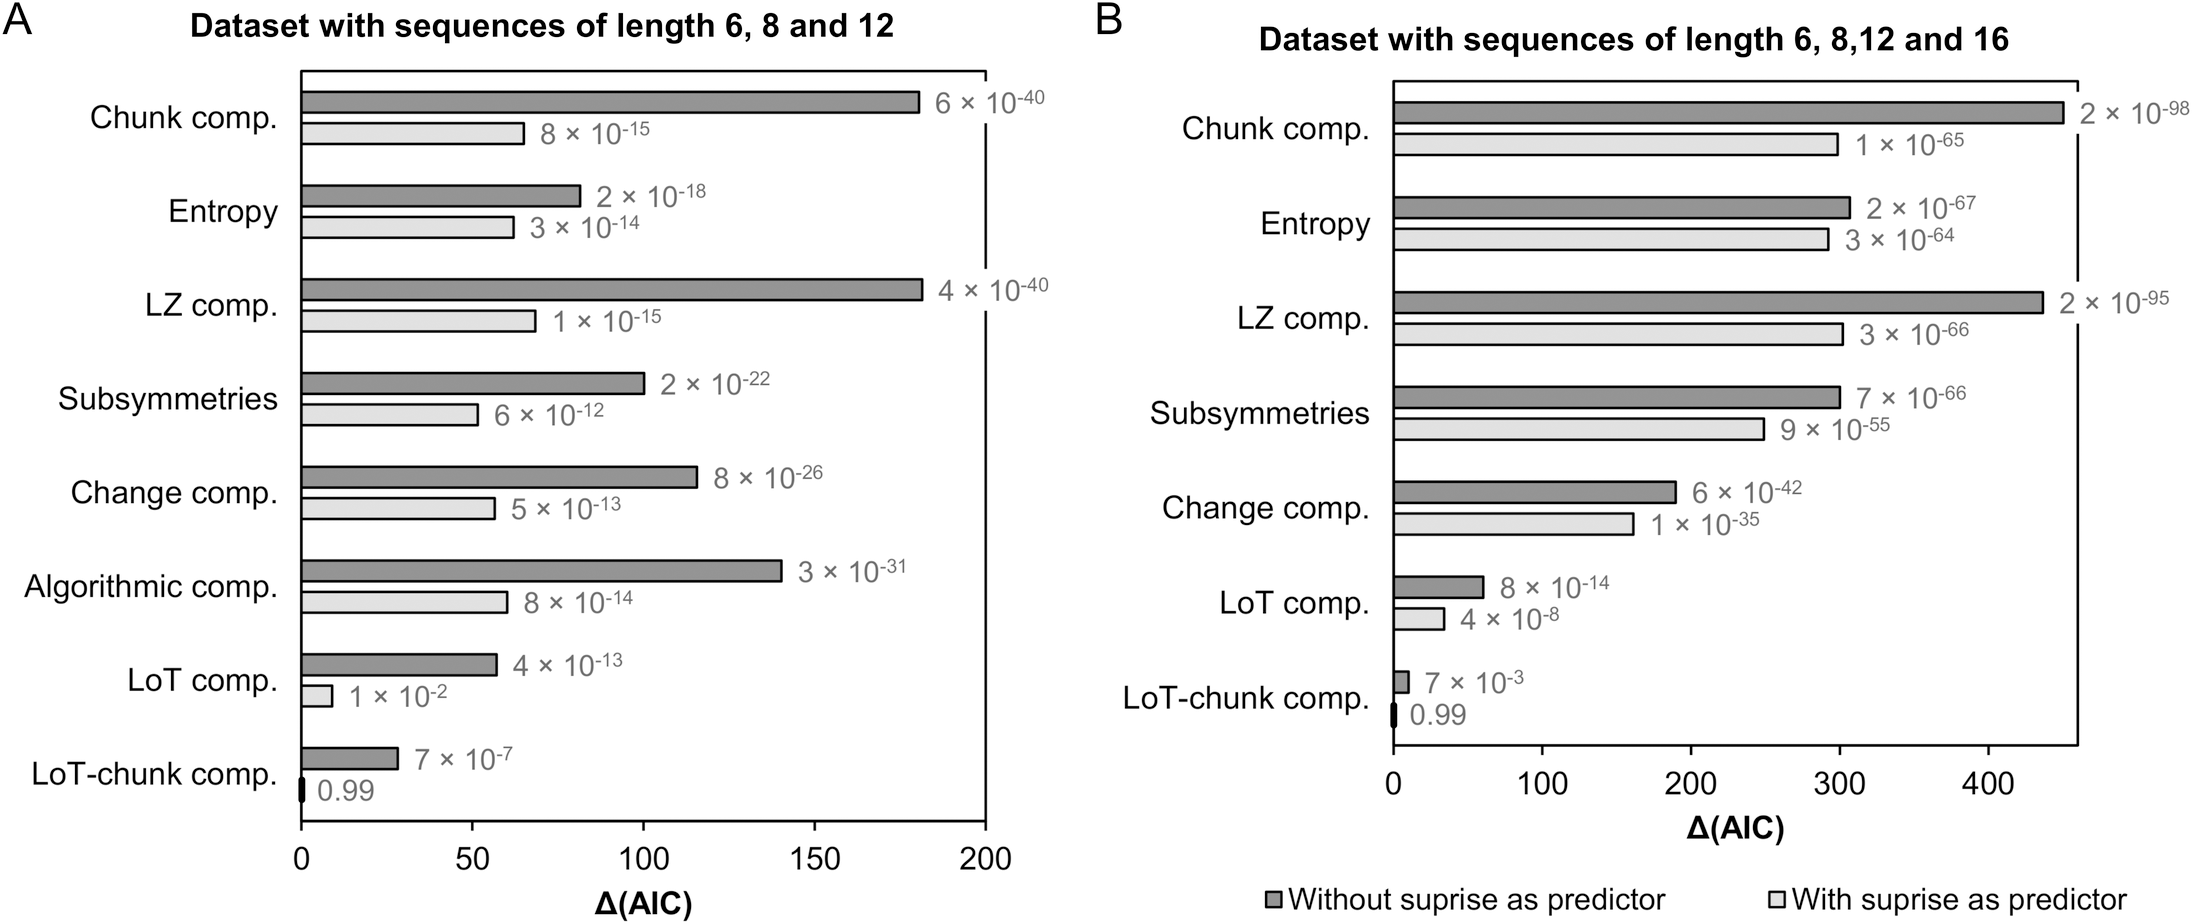
\includegraphics[scale=0.8]{figuras/plosbio/journal.pcbi.1008598.g008.PNG}
   
   \centering
   %%Figure 8: Δ(AIC) for the sixteen mixed models tested using the dataset including the task performance (LISAS) for sequences of length 6, 8 and 12 (A), and for the twelve different mixed models tested using the dataset with sequences of length 6, 8, 12 and 16 (B). The fixed effect of interest is indicated along the vertical axis (all models included participants as a random effect and could include surprise as a covariate — light gray bars). Akaike weight for each model is also reported. The model with lower AIC (Δ(AIC) = 0) is indicated by short dark vertical line on the vertical axis.
   
   \caption{$\Delta(AIC)$ para los dieciséis modelos mixtos probados utilizando el conjunto de datos que incluye el desempeño de la tarea (LISAS) para secuencias de longitud 6, 8 y 12 (A), y para los doce modelos mixtos diferentes probados utilizando el conjunto de datos de longitud 6, 8, 12 y 16 (B). El efecto fijo de interés se indica a lo largo del eje vertical (todos los modelos incluyen a los participantes como efecto aleatorio y pueden incluir la sorpresa como una covariable (barras de color gris claro). Se informa también el peso Akaike para cada modelo. El modelo con $AIC$ más bajo ($\Delta (AIC) = 0$) se indica con una línea vertical corta y oscura en el eje vertical}
   \label{PlosBIO-F8}
\end{figure}
\sergio{la figura no está traducida}

%Although correlations between performance and LoT complexity in experiments 2, 3 and 4 (lengths 6, 8 and 12) were small compared to experiment 1 (length 16), LoT complexity again appears as the best predictor of performance in the violation detection task with sequences of length ≤ 12. Notably, the constraint of excluding, for each pattern, the expressions that resulted in the splitting of a chunk (before the selection of shortest expression) improved the fit of behavioral data. This observation suggests that participants did not always find the best way of coding some patterns (best in the sense of the language of thought considered here) because of a propensity to perform an initial chunking solely based on consecutive runs of identical items. 

Aunque las correlaciones entre el rendimiento y la complejidad LoT en los experimentos 2, 3 y 4 (longitudes 6, 8 y 12) fueron pequeñas en comparación con el experimento 1 (longitud 16), la complejidad LoT vuelve a aparecer como el mejor predictor del rendimiento en la detección de infracciones para secuencias de longitud $\leq 12$. En particular, la complejidad LoT de fragmentos y su restricción de excluir para cada patrón las expresiones que resultan en la división de un fragmento (antes de la selección de la expresión más corta) mejoró el ajuste a los datos de comportamiento. Esta observación sugiere que los participantes no siempre encontraron la mejor manera de codificar algunos patrones (mejor en el sentido del lenguaje de pensamiento considerado aquí) debido a una propensión a realizar una fragmentación basada únicamente en ejecuciones consecutivas de elementos idénticos.

%The next best model was the one with the “number of subsymmetries” predictor (and including the surprise covariate), suggesting that it also provides a good measure of the psychological complexity of patterns. However, while this appeared true here using statistical models partially controlling for sequence length (i.e. by including participant index as a random factor, since each participant performed the task with only one given sequence length), this measure appears inappropriate to predict complexity across different lengths. Indeed, when we computed the Pearson correlation of average LISAS per sequence for the pooled dataset (sequences of length 6, 8 and 12), we obtained a positive correlation value of.39. Such positive correlation is in conflict with the presupposition that patterns containing more symmetries should be simpler. This is explained by the fact that the number of subsymmetries tends to increase with sequence length. These correlations were actually negative when each length was considered independently (r = –.44 for length 6; r = –.54 for length 8; and r = –.58 for length 12). This is illustrated in Figure 9, where the average LISAS for each sequence is presented in relation to each complexity measure (see also Fig. S9 and Fig. S10 for the equivalent with reaction times and miss rates). To summarize, although this measure is quite good in predicting the complexity of sequences for given length, it fails in predicting the variations in complexity across sequence lengths. 

El siguiente mejor modelo fue el que tenía al predictor de número de subsimetrías (incluyendo la covariable sorpresa), lo que sugiere que también proporciona una buena medida de la complejidad psicológica de los patrones. Sin embargo, si bien esto parecía cierto aquí usando modelos estadísticos que controlan parcialmente la longitud de la secuencia (es decir, al incluir el índice de los participantes como factor aleatorio, ya que cada participante realizó la tarea con una sola longitud de la secuencia), esta medida parece inapropiada para predecir la complejidad en diferentes longitudes. De hecho, cuando calculamos la correlación de Pearson de LISAS promedio por secuencia para el conjunto de datos agrupados (secuencias de longitud 6, 8 y 12), obtuvimos un valor positivo de correlación de $.39$. Tal correlación positiva está en conflicto con la presuposición de que los patrones que contienen más simetrías deberían ser más simples. Esto se explica por al hecho de que el número de subsimetrías tiende a aumentar con la longitud de la secuencia. Estas correlaciones fueron de hecho negativas cuando cada longitud se consideró de forma independiente ($r = -.44$ para la longitud 6; $r= –.54$ para la longitud 8; y $r = -.58$ para la longitud 12). Esto se ilustra en la Figura~\ref{PlosBIO-F9}, donde el LISAS promedio para cada secuencia se presenta en relación con cada medida de complejidad (ver también la Figura~\ref{PlosBIO-S6} y Figura~\ref{PlosBIO-S7} para el equivalente con tiempos de reacción y tasas de fallos). Para resumir, aunque esta medida es bastante buena para predecir la complejidad de las secuencias de una longitud dada, no es eficiente para predecir las variaciones en la complejidad debido al largo de la secuencia.

%Another similar limitation applies to algorithmic complexity, where the correlation observed across lengths (r = .79) is mostly explained by the fact that complexity values present excessive discontinuities with length: algorithmic complexity ranges roughly between 14 and 16 for length 6; between 19 and 23 for length 8; and between 31 and 35 for length 12 (see Figure 9). Such a massive increase in complexity with length is not consistent with behavior. Again, LoT complexity provides a better correlation with the present behavioral data across a large range of sequence lengths, because it correctly predicts that, for instance, some 6-items long sequences can be more complex than some 12-items ones (e.g. ABAAAB, LoT complexity = 10, means LISAS = 778 ms; AAAAAABBBBBB, LoT complexity = 6, mean LISAS = 766 ms).

Otra limitación similar se aplica a la complejidad algorítmica D(5), donde la correlación observada en todas las longitudes ($r = .79$) se debe principalmente a que este valor presenta discontinuidades excesivas con la longitud: la complejidad algorítmica D(5) varía aproximadamente entre 14 y 16 para la longitud 6; entre 19 y 23 para la longitud 8; y entre 31 y 35 para la longitud 12 (ver Figura~\ref{PlosBIO-F9}). Semejantes aumentos de complejidad con la longitud no son coherentes con el comportamiento. De nuevo, la complejidad LoT proporciona una mejor correlación con los datos actuales de comportamiento en una gran rango de longitudes de secuencia, porque predice correctamente que, por ejemplo, algunas secuencias de 6 elementos pueden ser más complejas que algunas de 12 elementos (ejemplo, ABAAAB, Complejidad LoT = 10, promedio LISAS = 778 ms; AAAAAABBBBBB, Complejidad LoT = 6, promedio LISAS = 766 ms).

\begin{table}[]
\centering
\resizebox{\textwidth}{!}{\begin{tabular}{lccccccccc}
\hline
\textit{}               & \multicolumn{4}{l}{\textit{\textbf{Datos para secuencias de longitud 6, 8 y 12}}} & \multicolumn{1}{l}{}     & \multicolumn{4}{l}{\textit{\textbf{Datos para secuencias de longitud 6, 8, 12 y 16}}} \\
\textit{Modelo de efectos fijos}   & \textit{Log-lik.}  & $\Delta(AIC)$  & $\Delta(BIC)$  & $w(AIC)$  & \multicolumn{1}{l}{\textit{}} & \textit{Log-lik.}   & $\Delta(AIC)$   & \textit{$\Delta$(BIC)}  & \textit{w(AIC)}  \\ \hline
\textit{Comp. LoT}          & -14886        & 57         & 51        & 4.0 × 10-13    &                & -16653        & 60         & 55         & 7.8 × 10-14    \\
\textit{Comp. LoT + Sorpresa}     & -14861        & 9         & 9         & 1.1 × 10-2    &                & -16639        & 34         & 34         & 4.1 × 10-8     \\
\textit{Comp. Lot Fragm.}       & -14872        & 28         & 23        & 7.4 × 10-7    &                & -16628        & 10         & 4         & 6.8 × 10-3     \\
\textit{Comp. Lot Fragm. + Sorpresa} & -14857        & 0         & 0         & 0.99       &                & -16622        & 0          & 0         & 0.99        \\
\textit{Comp. Fragmentos}       & -14948        & 180        & 175        & 6.4 × 10-40    &                & -16848        & 450         & 445        & 1.6 × 10-98    \\
\textit{Comp. Fragmentos + Sorpresa} & -14889        & 65         & 65        & 7.5 × 10-15    &                & -16771        & 299         & 299        & 1.4 × 10-65    \\
\textit{Entropía}           & -14899        & 81         & 76        & 2.0 × 10-18    &                & -16776        & 307         & 301        & 2.3 × 10-67    \\
\textit{Entropía + Sorpresa}     & -14888        & 62         & 62        & 3.4 × 10-14    &                & -16768        & 292         & 292        & 3.3 × 10-64    \\
\textit{Comp. LZ}           & -14948        & 181        & 176        & 3.9 × 10-40    &                & -16841        & 436         & 431        & 1.6 × 10-95    \\
\textit{Comp. LZ + Sorpresa}     & -14891        & 68         & 68        & 1.4 × 10-15    &                & -16773        & 302         & 302        & 2.6 × 10-66    \\
\textit{Subsimetrías}         & -14908        & 100        & 94        & 1.2 × 10-22    &                & -16773        & 300         & 294        & 8.8 × 10-55    \\
\textit{Subsimetrías + Sorpesa}    & -14883        & 52         & 52        & 6.2 × 10-12    &                & -16746        & 249         & 249        & 1.3 × 10-17    \\
\textit{Comp. de cambio}       & -14916        & 116        & 110        & 7.6 × 10-26    &                & -16718        & 190         & 184        & 6.2 × 10-42    \\
\textit{Comp. de cambio + Sorpresa}  & -14885        & 57         & 57        & 5.3 × 10-13    &                & -16703        & 161         & 161        & 1.0 × 10-35    \\
\textit{Comp. Algorítmica}      & -14928        & 140        & 135        & 3.4 × 10-31    &                & \multicolumn{4}{c}{N.D.}                               \\
\textit{Comp. Algorítmica + Sorpresa} & -14887        & 60         & 60        & 8.4 × 10-14    &                & \multicolumn{4}{c}{N.D.}                               \\ \hline
\end{tabular}}
%Note. All models included participants as a random effect, and either one or two fixed effect(s) (i.e. “+ Surp.”: with additional surprise fixed effect). Log-lik. = log of the maximum likelihood for the model. Δ(AIC) = AIC difference with the model with the lowest AIC value (where AIC is the Akaike Information Criterion). Δ(BIC) = BIC difference with the model with the lowest BIC value (where BIC is the Bayesian Information Criterion). w(AIC) = Akaike weight.

\caption{Todos los modelos incluyeron a los participantes como efecto aleatorio y uno o dos efectos fijos (es decir, ``+ Sorpresa'' como efecto fijo sorpresa adicional). Log-lik. = logaritmo de la máxima verosimilitud del modelo. $\Delta (AIC)$ = Diferencia $AIC$ del modelo con el valor de $AIC$ más bajo (donde $AIC$ es el criterio de información de Akaike). $\Delta (BIC)$ = Diferencia BIC del modelo con el valor $BIC$ más bajo (donde $BIC$ es el criterio de información bayesiano). $w(AIC)$ = peso Akaike}
\label{PlosBIO-T2}
\end{table}


\subsection{Datos para secuencias de longitud 6, 8 y 12}

%Fourteen different mixed models (with participants as a random effect) were here fitted, using the same dataset as before to which was added data from 11 sequences for which algorithmic complexity value was not available (thus now with sequences of length 6, 8, 12 and 16). The same predictors as above were used, with the exception of algorithmic complexity. Here again, as illustrated in Figure 8B, goodness of fit systematically increased when surprise was included. LoT-chunk complexity and LoT complexity (with or without surprise as a covariate) were again the best predictors of performance (see Table 2). As opposed to the previous set of analyses in which the data from experiment 1 (length 16) was not included, the model with change complexity performed clearly better than the one with the number of subsymmetries. The long sequences used in experiment 1 indeed presented important differences in their number of subsymmetries (e.g. 56 for (AB)8 vs. 32 for (A4B4)2), which were clearly not predictive of performance. Consequently, and as stated earlier, the number of subsymmetries does not appear as a good predictor of task performance across different sequence lengths. Change complexity also appeared as a much better predictor when performing a simple linear regression on average LISAS per sequence (see Figure 9), resulting in an r = .81, which is close to the one obtained with LoT complexity (r = .82). It indicates that change complexity can also be a good measure of the psychological complexity of a sequence regardless of its length. It must however be noted that, contrary to mixed models, these linear regressions using data averaged over participants did not control for the variance accounted for by surprise, or due to inter-subject variability. Important variations in the correlation with complexity (especially for experiments with shorter sequences) were indeed observed across participants. When computed at the level of individual participants, the correlation with LoT complexity appeared on average stronger (mean r = .31, SD = .32) than the one with change complexity (mean r = .23, SD = .30; t(112) = 3.54, p < .001).

Aquí se ajustaron catorce modelos mixtos diferentes (con participantes como efecto aleatorio), utilizando el mismo conjunto de datos que antes al que se le agregaron los datos de 11 secuencias para las cuales el valor de complejidad algorítmica D(5) no estaba disponible (por lo tanto, ahora son secuencias de longitud 6, 8, 12 y 16). Se utilizaron los mismos predictores que antes, con la excepción de la complejidad algorítmica D(5). Aquí nuevamente, como se ilustra en la Figura~\ref{PlosBIO-F8}B, el ajuste mejoró sistemáticamente cuando se incluyó la sorpresa. La complejidad LoT de fragmentos y la complejidad oT (con o sin sorpresa como covariable) fueron nuevamente los mejores predictores del desempeño (ver Tabla~\ref{PlosBIO-T2}). En contraposición al conjunto anterior de análisis en el que los datos del experimento 1 (longitud 16) no se incluyeron, el modelo con complejidad de cambio se desempeñó claramente mejor que el que utiliza el número de subsimetrías. Las secuencias utilizadas en el experimento 1 de hecho presentaron diferencias importantes en su número de subsimetrías (por ejemplo, 56 para $(AB)^8$ vs. 32 para $(A^4B^4)^2$), que claramente no eran predictivas del rendimiento. En consecuencia, y como se dijo anteriormente, el número de subsimetrías no parece ser un buen predictor para el desempeño en diferentes longitudes de secuencia. La complejidad del cambio también apareció como un predictor mucho mejor cuando se realizan regresiones lineales simples en los promedios LISAS por secuencia (ver Figura~\ref{PlosBIO-F9}), resultando en una $r = .81$, que es cercana a la obtenida con complejidad LoT ($r = .82$). Esto indica que la complejidad del cambio también puede ser una buena medida de la complejidad psicológica de una secuencia independientemente de su longitud. Sin embargo, cabe señalar que, a diferencia de los modelos mixtos, estas regresiones lineales que utilizan datos promediados sobre los participantes no controló la varianza explicada por sorpresa, o la variabilidad entre sujetos. De hecho, se observaron variaciones importantes entre participantes con respecto a la correlación con la complejidad (especialmente para experimentos con secuencias más cortas). Cuando se calcula a nivel de participantes individuales, la correlación con la complejidad LoT apareció en promedio más fuerte (media $r = .31, SD = .32$) que la complejidad de cambio (media $r = .23, SD = .30$) ($t (112) = 3.54, p < .0006$)

%With both datasets, two measures performed poorly, LZ complexity and chunk complexity. Contrary to our language, the LZ algorithm has the advantage to be able to quickly “parse” any sequence of any number of different characters, by building for each sequence its own vocabulary of substrings. Its adequacy to human behavior, however, appears limited since, when scanning the sequence from one item to the next, it does not necessarily take into consideration runs of repeated items (AAA can be described with two substrings, A and AA) and fails to capture repeating patterns. This deficiency is especially striking for a low LoT complexity sequence such as (A2B2)4 (i.e. AABBAABB…), where 8 substrings are present in the vocabulary at the end of scanning (the first four substrings encountered by the algorithm are A, AB, B, AA). This gives this sequence the lower level of LZ compressibility among those tested, which is clearly not predictive of performance.

Con ambos conjuntos de datos, dos medidas tuvieron un desempeño deficiente: la complejidad LZ y la complejidad de fragmentos. Al contrario de nuestro lenguaje, el algoritmo LZ tiene la ventaja de poder ``analizar'' rápidamente cualquier secuencia de cualquier número de caracteres diferentes, construyendo para cada secuencia su propio vocabulario de subcadenas. Su adecuación al comportamiento humano, sin embargo, parece limitada. Esto se debe a que, al escanear la secuencia de un elemento al siguiente, no necesariamente tiene en cuenta trazas de elementos repetidos (``AAA'' se puede describir con dos subcadenas, ``A''y ``AA'') y no logra capturar algunos patrones repetidos. Esta deficiencia es especialmente llamativa para una secuencia de baja complejidad LoT como $(A^2B^2)^4$ (es decir, AABBAABB$\cdot$), donde 8 subcadenas están presentes en el vocabulario al final del escaneo (las primeras cuatro subcadenas encontradas por el algoritmo son ``A'', ``AB'', ``B'',``AA''). Esto le da a esta secuencia el nivel más bajo de compresibilidad LZ entre los probados, que claramente no es predictivo de su rendimiento.

%Similarly, “chunk complexity”, like other methods solely based on quantifying chunks (number of chunks, chunks length, or a combination of both), is strongly dependent on how chunks are defined. Here, since chunks are defined as runs of identical items, the complexity of sequences containing alternations tends to be overestimated (e.g. ABABABAB has 8 chunks). Assessing complexity based on chunks therefore requires first building a model that defines what chunks are for the sequence processing cognitive system, which is not trivial. Another limitation of this measure is an excessive sensitivity to sequence length. In the absence of any recursive compression, complexity increases linearly with the number of chunks. Allowing compression based on consecutive repetitions of chunks (chunks of chunks), as in the LoT model proposed here, appears to be a better strategy for predicting the subjective complexity of sequences. Note that, notwithstanding the aforementioned concerns, change complexity captures relatively well the complexity variations due to both structure and length (Figure 9). This may be due to the fact that change complexity is computed within substrings of all possible lengths, which is another way to capture regularities at multiple hierarchical levels.

Del mismo modo, la complejidad de fragmentos, al igual que otros métodos basados únicamente en la cuantificación de fragmentos (número de trazas, longitud de trazas o una combinación de ambos), depende en gran medida de cómo las trazas están definidas. Aquí, dado que los fragmentos se definen como ejecuciones de elementos idénticos, la complejidad de secuencias que contienen alternancias tiende a sobreestimarse (por ejemplo, ``ABABABAB'' tiene 8 trazas). Evaluar la complejidad basada en fragmentos, por lo tanto, requiere primero construir un modelo que defina qué son los fragmentos para el sistema cognitivo de procesamiento de secuencias, lo cual no es trivial. Otra limitación de esta medida es una sensibilidad excesiva al largo de la secuencia. En ausencia de cualquier mecanismo de compresión recursiva, la complejidad aumenta linealmente con el número de trazas. Permitir la compresión basada en repeticiones consecutivas de fragmentos (trazas de trazas), como en el modelo LoT propuesto aquí, parece ser una mejor estrategia para predecir la complejidad subjetiva de las secuencias. Se debe tener en cuenta que, a pesar de las dificultades mencionadas, la complejidad del cambio captura relativamente bien las variaciones de complejidad relacionadas tanto a la estructura como a la longitud (Figura~\ref{PlosBIO-F9}). Esto puede deberse al hecho de que la complejidad del cambio se calcula dentro de las subcadenas de todas las longitudes posibles, que es otra forma de capturar regularidades en múltiples niveles jerárquicos.

%Unlike several other experimenters, we used an objective deviant detection task to index the psychological complexity of auditory and visual patterns. However, we also collected subjective complexity rating in experiment 1 and 2 (with respectively 10 and 12 sequences), which we therefore also fitted to the various models. In experiment 1, the results were quite consistent in favoring LoT complexity (r = .99 for deviant detection, r= .94 for subjective complexity rating), LoT-chunk complexity (r = .99 and r= .93) and change complexity (r = .89 and r= .95), while entropy (r= .58 and r= .70) and subsymmetries (r = -.63 and r=-.82) led to lower and less consistent results. Similarly in experiment 2, the correlations were good with LoT complexity (r = .60 for deviant detection, r= .61 for subjective complexity rating) and Lot chunk complexity (r = .72 and r= .71), but surprisingly, other measures now provided equally good or even better fits: change complexity (r= .28 vs. r= .65) and especially entropy (r= .43 vs. r= .78) and subsymmetries (r=-.44 vs. r=-.85). Although these results must be treated with caution since they come from a relatively small number of sequences and trials, they may indicate that the internal code for sequences is not entirely accessible to introspection and that, therefore, subjective ratings do not always faithfully reflect the subjects’ objective memory abilities.

A diferencia de otros experimentadores, utilizamos una tarea de detección objetiva de desviaciones para indexar la complejidad psicológica de los patrones auditivos y visuales. Sin embargo, también recopilamos la clasificación de complejidad subjetiva en el experimento 1 y 2 (con 10 y 12 secuencias respectivamente), que también ajustamos a los diversos modelos. En el experimento 1, los resultados fueron bastante consistentes a favor de la complejidad LoT ($r = .99$ para la detección de desviaciones, $r = .94$ para la calificación de complejidad subjetiva), la complejidad LoT de fragmento ($r = .99$ y $r = .93$) y la complejidad del cambio ($r = .89$ y $r = .95$), mientras que la entropía ($r = .58$ y $r = .70$) y las subsimetrías ($r = -.63$ y $r = -.82$) llevaron a resultados más bajos y menos consistentes. De manera similar, en el experimento 2, las correlaciones fueron buenas con la complejidad LoT ($r = .60$ para la detección de desviaciones, $r = .61$ para la calificación de complejidad subjetiva) y la complejidad LoT de fragmentos ($r = .72$ y $r = .71$), pero sorprendentemente las otras medidas ahora proporcionaron ajustes igualmente buenos o incluso mejores: complejidad del cambio ($r = .28$ vs $r = .65$) y especialmente entropía ($r = .43$ vs $r = .78$) y subsimetrías ($r = -. 44$ vs $r = -. 85$). Aunque estos resultados deben tratarse con precaución ya que provienen de un número relativamente pequeño de secuencias y ensayos, pueden indicar que el código interno de las secuencias no es completamente accesible a la introspección y que, por lo tanto, las calificaciones subjetivas no siempre reflejan fielmente a las habilidades objetivas de memoria de los sujetos.



\widesanti{Este párrafo que sigue vino por una crítica de un reviewer. Está muy bien, pero lo aislaría en una sección o subsección para destacarlo. Es una justificación y defensa de la metodología.}
%It could be argued that the above results may be biased because we started with a preconceived language-of-thought and selected sequences whose structures were well-captured by that language (as well as some sequences that were maximally irregular according to that language). Although such a bias cannot be definitively ruled out, there are several arguments against it.. First, this potential problem does not apply to experiments 3 and 4, where we tested all appropriate sequences of length 6 and 8, in an unbiased manner (the only restriction for sequences of length 8 was to have the same number of As and Bs). An additional model comparison analysis, restricted to those sequences, revealed that our complexity metrics remained the best predictors (see Fig. 10A). Very similar results were obtained when including only the set of length-8 sequences, which appears to be the minimum length at which compression effects have been observed (see Fig. S11). Second, for longer sequences, exhaustive sampling would have been impossible, and random sampling would have been equally inappropriate. This is because for any reasonable notion of complexity, only a very small number of sequences achieve a low complexity, while the vast majority of randomly selected sequences achieve a high level of complexity (43,li2013introduction). Thus, some selection of sequences was required in experiments 1 and 2, with length 16 and length 12 respectively. The graphs in figure 9 nevertheless indicate that our selection was not particularly biased, inasmuch as the values of, for instance, change complexity or entropy spanned across a broad range and therefore would have permitted those variables to win over LoT complexity in our regressions, if they had been the best predictors. In spite of this relative “theory neutrality” of our length-12 and length-16 sequences, we again found an advantage in favor of the LoT and LoT-chunk predictors (Fig. 10B) when model comparison was restricted to them. Furthermore, even when restricting the analysis to a subsample of thirteen length-12 and length-16 sequences for which change complexity was approximately constant (between 5 and 7), we still found a correlation of performance with LoT-Chunk complexity (r=0.70, p=0.007) and a marginal one with LoT complexity (r = 0.54, p=0.057), while the correlation with change complexity was naturally no longer present, r = .23, p = .45). Finally, note that although our research was indeed initially predicated on the idea that LoT complexity would be the best predictor of human behavior, the data was unbiased enough to lead to a different conclusion, namely that Lot-chunk complexity was a superior predictor. Nevertheless, we acknowledge that our experiments were not specifically designed to arbitrate between different models of sequence complexity with respect to their capacity to predict behavior (especially regarding the selection of the longer sequences). The set of long sequences used here represents only a tiny sample of all possible combinations and structures and, in spite of the above arguments, it cannot be definitely excluded that models other than ours would be better at capturing psychological complexity if a different set was used. Future studies could focus on the isolation of sequences for which different models make opposite predictions. Such a situation, although relatively rare (because different complexity metrics tend to correlate with each other) may exist within the large number of available sequences and should provide more definitive data.

Se podría argumentar que los resultados anteriores pueden estar sesgados porque comenzamos con un lenguaje de pensamiento preconcebido y secuencias seleccionadas cuyas estructuras fueron bien capturadas por ese lenguaje (así como algunas secuencias que eran máximamente irregulares según ese lenguaje).\santi{quizá acá convenga un comentario en relación al cap 2} Aunque tal sesgo no puede descartarse definitivamente, existen varios argumentos en contra. Primero, este problema potencial no se aplica a los experimentos 3 y 4, donde probamos todas las secuencias apropiadas de longitud 6 y 8, de una manera no sesgada (la única restricción para las secuencias de longitud 8 fue tener el mismo número de As y Bs). Un análisis de comparación de modelos adicional, restringido a esas secuencias, reveló que nuestras métricas de complejidad seguían siendo los mejores predictores (ver Figura~\ref{PlosBIO-F10}A). Se obtuvieron resultados muy similares al incluir sólo el conjunto de secuencias de longitud 8, que parece ser la longitud mínima para la que se han observado efectos de compresión (ver Figura\ref{PlosBIO-S11}). En segundo lugar, para secuencias más largas, el muestreo exhaustivo habría sido imposible y el muestreo aleatorio habría sido igualmente inapropiado. Esto se debe a que para cualquier noción razonable de complejidad, solo un número muy pequeño de secuencias logran una complejidad baja, \santi{aca citar resultado que está en la intro que dice que la gran mayoría de las secuencias tiene alta complejidad ***}mientras que la gran mayoría de secuencias seleccionadas al azar logran un alto nivel de complejidad~\cite{f43,li2013introduction}. Por tanto, se requirió alguna selección de secuencias en los experimentos 1 y 2, con longitudes 16 y longitudes 12 respectivamente. No obstante, los gráficos de la Figura~\ref{PlosBIO-F9} indican que nuestra selección no fue particularmente sesgada ya que los valores de, por ejemplo, la complejidad de cambio o la entropía se extendieron a lo largo de un amplio rango y, por lo tanto, habrían permitido que esas variables ganaran\santi{revisar redacción} respecto de la complejidad LoT en nuestras regresiones si hubieran sido los mejores predictores. A pesar de esta relativa ``neutralidad teórica'' de nuestras secuencias de longitud 12 y longitud 16, nuevamente encontramos una ventaja a favor de los predictores de complejidad LoT y complejidad LoT de fragmentos (Figura~\ref{PlosBIO-F10}B) cuando la comparación de modelos se restringió a ellos. Además, incluso al restringir el análisis a una submuestra de trece secuencias de longitud 12 y longitud 16 para las que la complejidad del cambio era aproximadamente constante (entre 5 y 7), todavía encontramos una correlación del rendimiento con la complejidad LoT de fragmentos ($r = 0,70, p = 0,007$) y una marginal con la complejidad LoT ($r = 0,54, p = 0,057$), mientras que la correlación con la complejidad del cambio naturalmente ya no estaba presente ($r = .23, p = .45$). Finalmente, se debe tener en cuenta que, aunque nuestra investigación se basó inicialmente en la idea de que la complejidad LoT sería el mejor predictor del comportamiento humano, los datos fueron lo suficientemente imparciales como para llevar a una conclusión diferente: la complejidad LoT de fragmentos resultó un predictor superior. Sin embargo, reconocemos que nuestros experimentos no fueron diseñados específicamente para arbitrar entre diferentes modelos de complejidad de secuencias con respecto a su capacidad para predecir el comportamiento (especialmente en lo que respecta a la selección de secuencias más largas). El conjunto de secuencias largas utilizadas aquí representa sólo una pequeña muestra de todas las combinaciones y estructuras posibles y, a pesar de los argumentos anteriores, no se puede excluir definitivamente que modelos distintos al nuestro resulten mejores para capturar la complejidad psicológica si se utilizara un conjunto diferente. Los estudios futuros podrían centrarse en el aislamiento de secuencias para las que diferentes modelos hacen predicciones opuestas. Tal situación, aunque relativamente rara (porque las diferentes métricas de complejidad tienden a correlacionarse entre sí) puede existir dentro del alto número de secuencias disponibles y debería proporcionar datos más definitivos.

\begin{figure}[t!]
   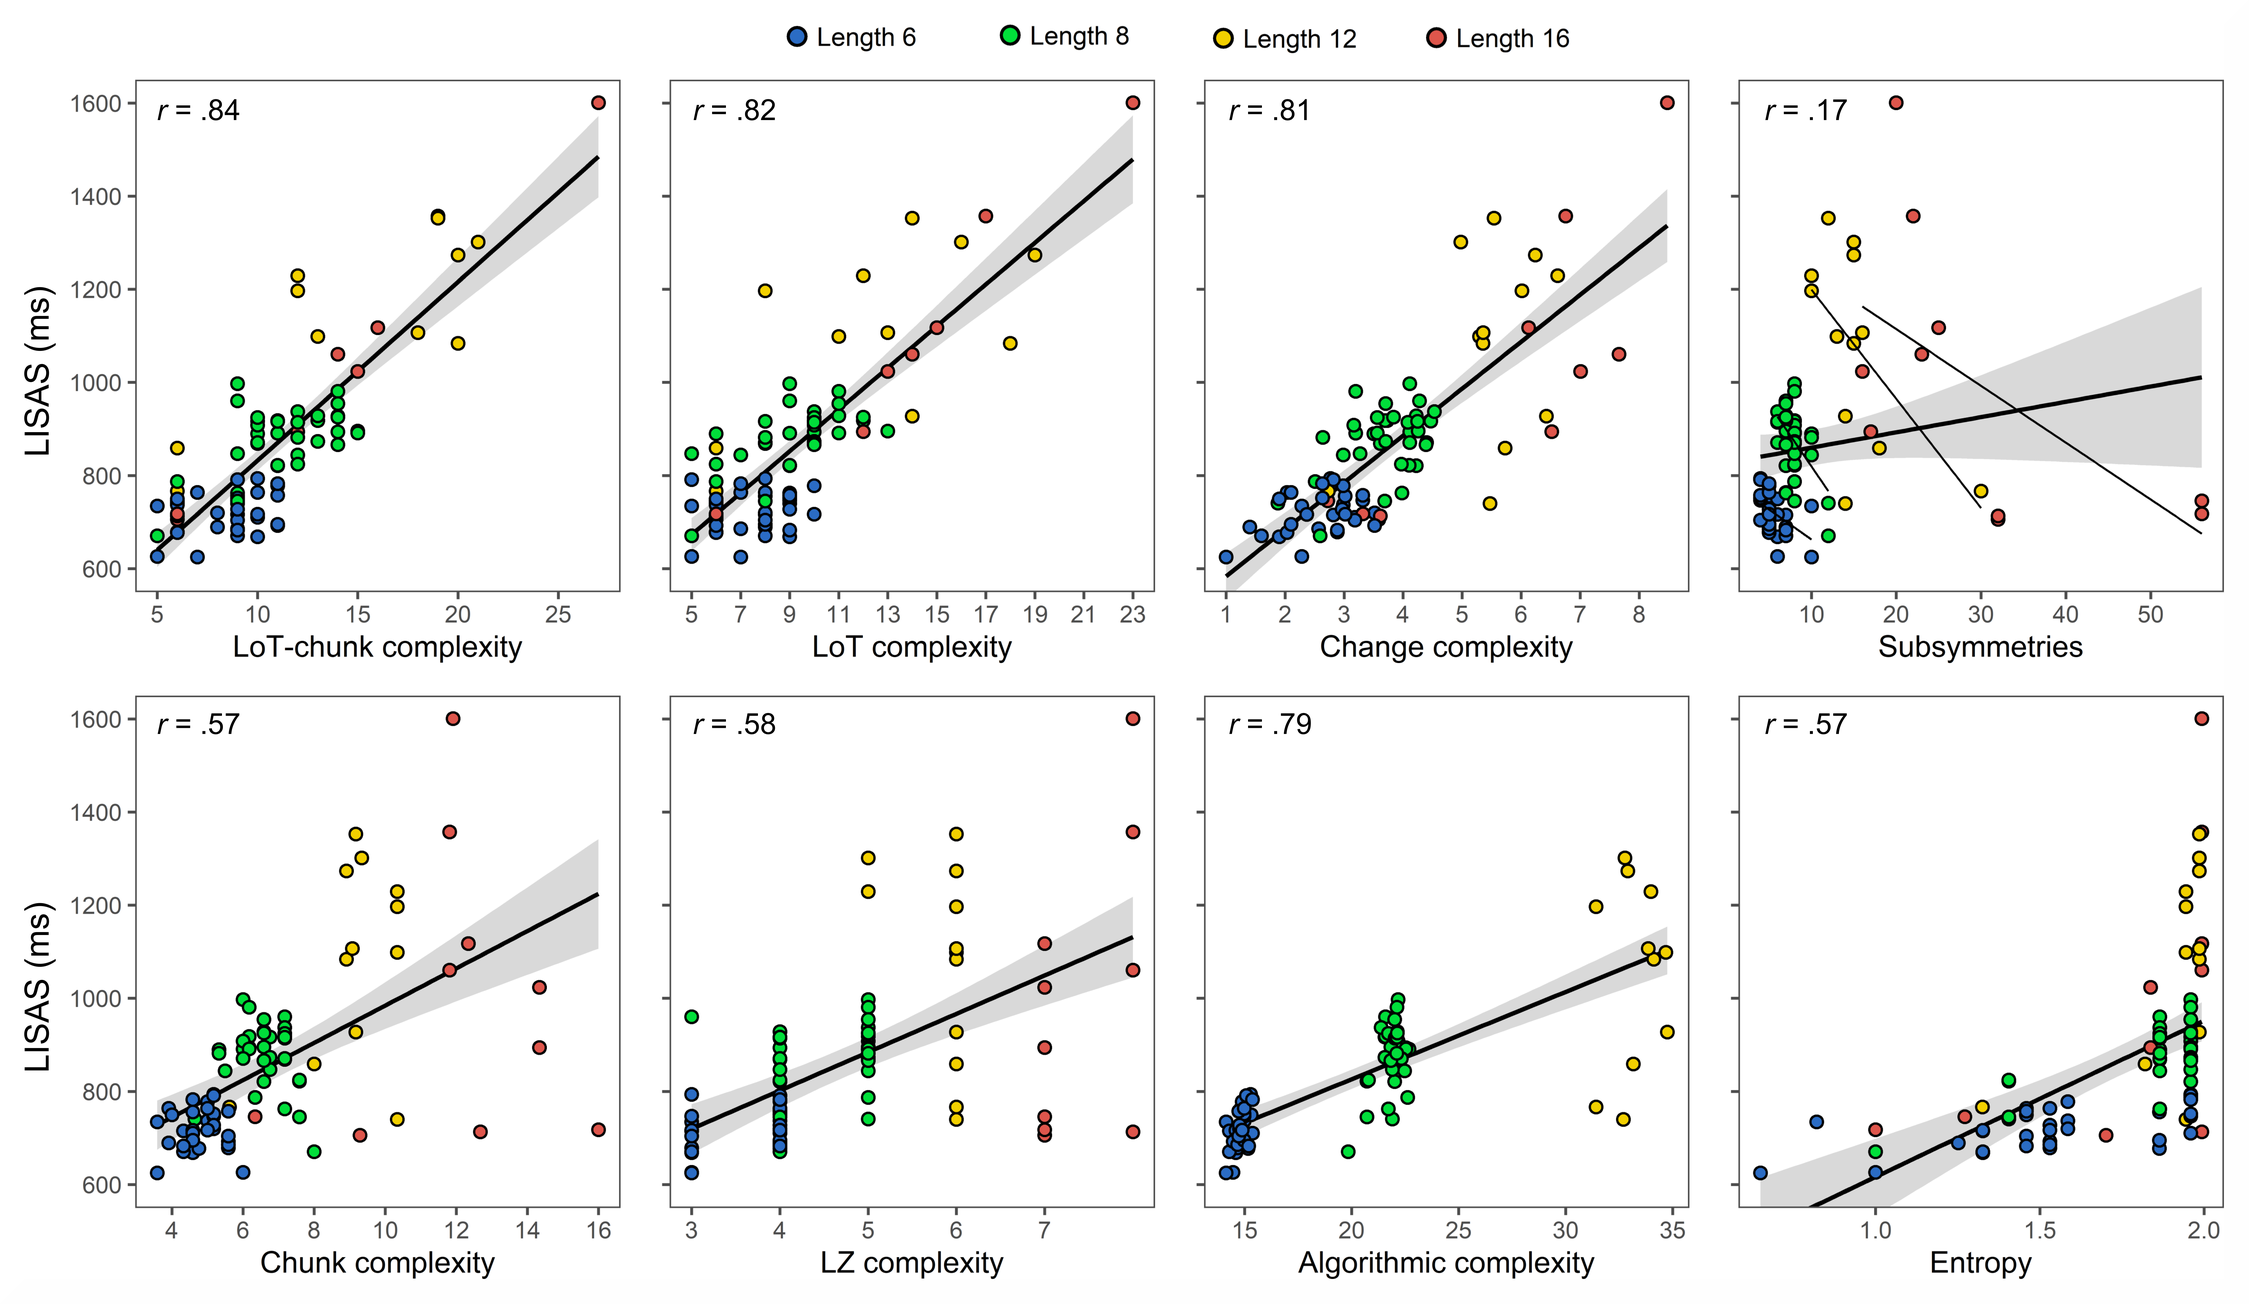
\includegraphics[scale=0.8]{figuras/plosbio/journal.pcbi.1008598.g009.PNG}
   
   \centering
   %%Figure 9: Linear regressions of average performance per sequence (LISAS, in ms) with eight different predictors of interest when combining data from experiments with auditory sequences of 4 different lengths. Each marker corresponds to one sequence. Sequences of different lengths are indicated by different markers only for illustration purposes (the length factor was not taken into account when computing the correlation coefficient, r). 16-items long sequences (as well as one 12-items sequence) could not be included in the regression with algorithmic complexity. Regressions lines for each sequence length were added in the subsymmetries plot, in order to illustrate the fact that negative correlations were observed when each length was considered separately. Note that the average performance data presented here does not take into account the effects of surprise, inter-subject, or inter-experiment variability.

   \caption{Regresiones lineas de rendimiento promedio por secuencia (LISAS, en ms.) con ocho predictores diferentes de interés al combinar datos de experimentos con secuencias auditivas de 4 longitudes diferentes. Cada marcador corresponde a una secuencia. Las secuencias de diferentes longitudes se indican con diferentes marcadores sólo a modo de ilustración (el factor de longitud no se tuvo en cuenta al calcular el coeficiente de correlación, r). Las secuencias de 16 elementos (así como una secuencia de 12 elementos) no se pudieron incluir en la regresión con complejidad algorítmica. Las líneas de regresión para cada longitud de secuencia se agregaron en el gráfico de subsimetrías con el fin de ilustrar que se observaron correlaciones negativas cuando se consideró cada longitud por separado. Notar que los datos de rendimiento promedio presentados aquí no tienen en cuenta los efectos de sorpresa o variabilidad entre sujetos o entre experimentos}
   \label{PlosBIO-F9}
\end{figure}
\sergio{la figura no está traducida}

\begin{figure}[t!]
   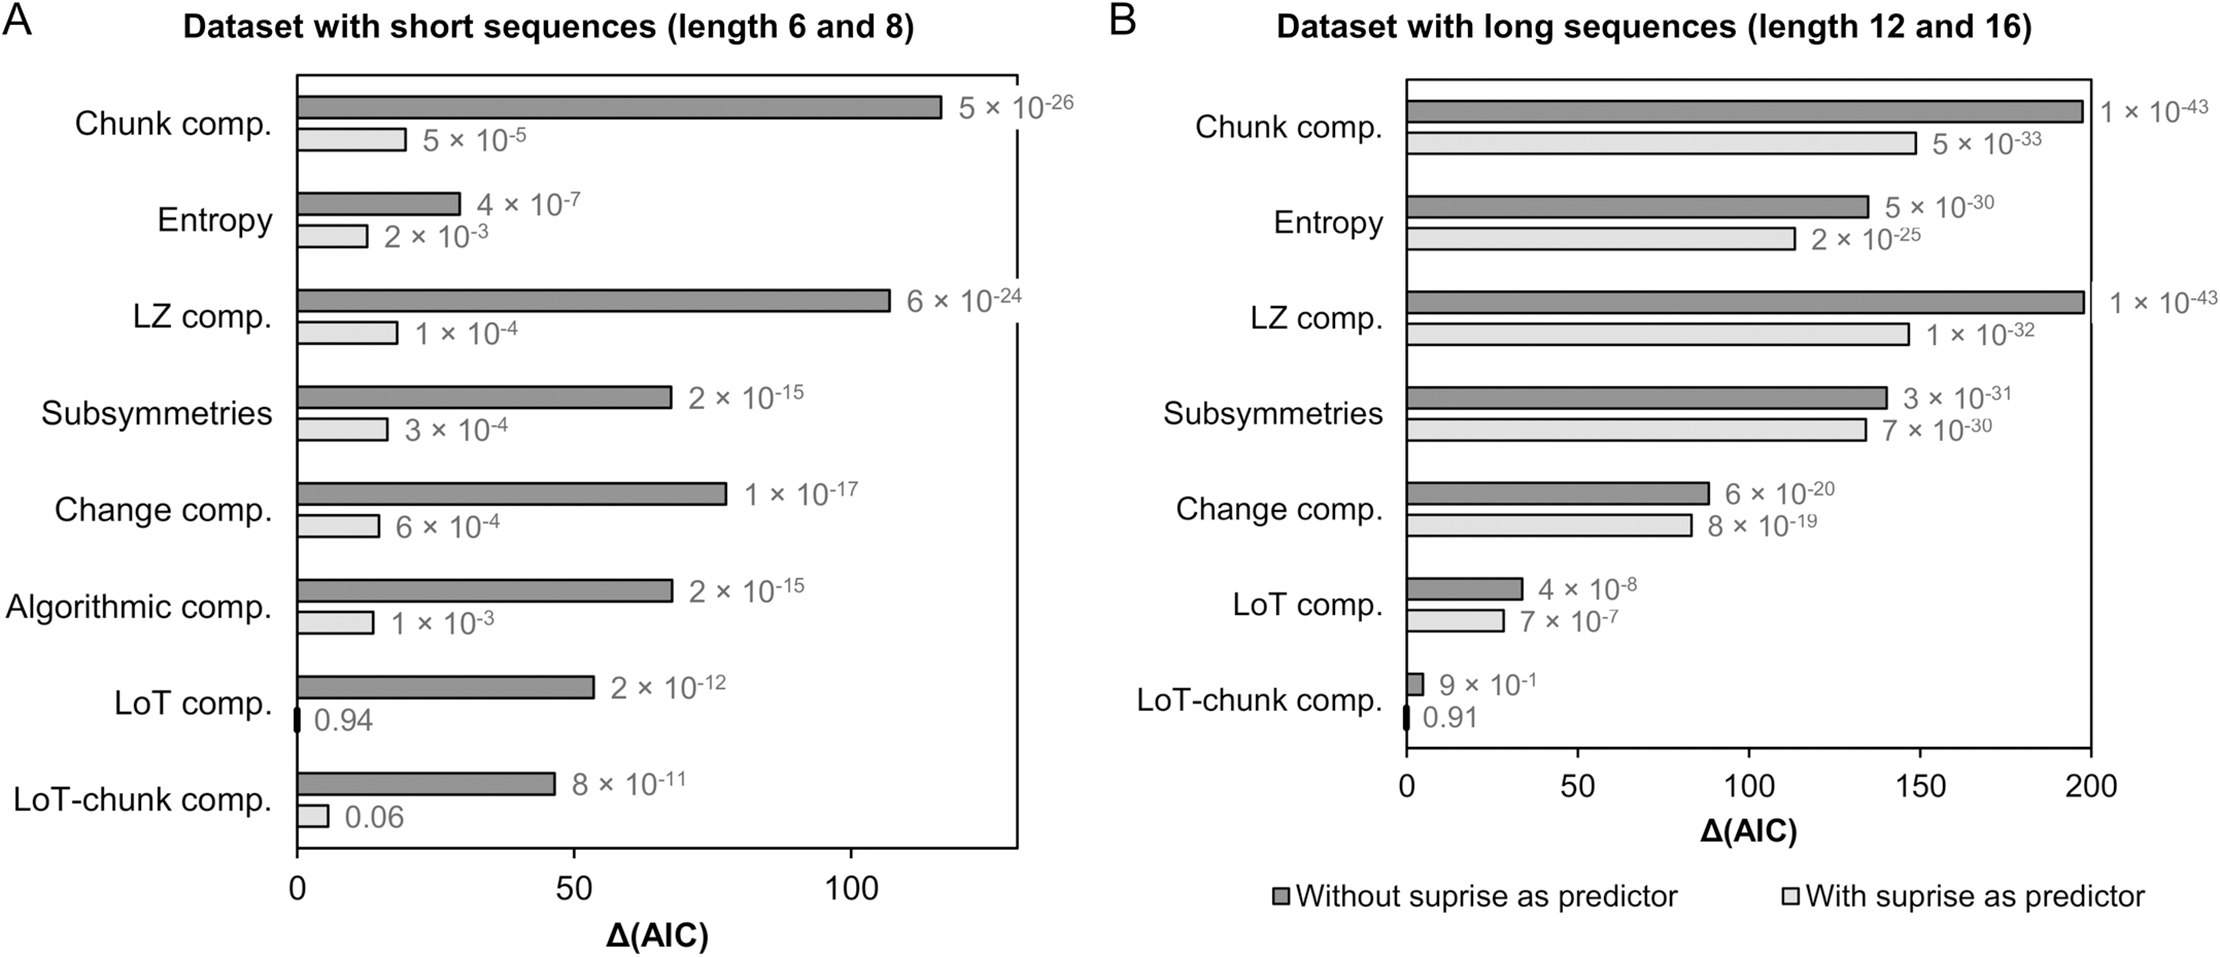
\includegraphics[scale=0.8]{figuras/plosbio/journal.pcbi.1008598.g010.PNG}
   
   \centering
   %%Figure 10: Complementary mixed model comparison with two pooled dataset. A) Δ(AIC) for the sixteen mixed models tested using a dataset including the task performance (LISAS) for sequences of length 6 and 8 (66 sequences) (A), and for the twelve different mixed models tested using the dataset with sequences of length 12 and 16 (22 sequences) (B). The fixed effect of interest is indicated along the vertical axis (all models included participants as a random effect and could include surprise as a covariate — light gray bars). Akaike weight for each model is also reported.
   
   \caption{Comparación de modelo mixto con dos conjuntos de datos. (A) $\Delta(AIC)$ para los dieciséis modelos mixtos probados usando un conjunto de datos que incluye el desempeño de la tarea (LISAS) para secuencias de longitud 6 y 8 (66 secuencias), y (B) para los doce modelos mixtos diferentes probados usando el conjunto de datos con secuencias de longitud 12 y 16 (22 secuencias). El efecto fijo de interés se indica a lo largo del eje vertical (todos los modelos incluyeron a los participantes como efecto aleatorio y podrían incluir la sorpresa como una covariable: barras de color gris claro). También se informa el peso de Akaike para cada modelo}
   \label{PlosBIO-F10}
\end{figure}
\sergio{la figura no está traducida}

\section{Discusión General}

%The main goal of this series of experiments was to evaluate the mental representation of binary sequences and to test the adequacy of a formal language of thought previously proposed to account for geometrical sequences (58). Similar models were proposed in the past (e.g. 32,36,45) but were not submitted to a full experimental validation, particularly in comparison to the most recent approaches of sequence complexity. Moreover, we sought to distinguish the effects related to statistical transition-probability learning, which are unavoidable when dealing with temporal sequences of stimuli, from the putative influence of rule-based encoding. Across five different experiments with sequences of different lengths, in the auditory but also in the visual modality, we found consistent evidence that, a significant part of the variations in sequence encoding performance (as indexed by the capacity to detect sequence violations) was explained by the length of the shortest possible description of the sequence in the proposed formal language (i.e. LoT complexity). This was however not the case for very short sequences (6 items). These results are consistent with the idea that upon hearing or seeing a binary sequence, when the number of items exceeds working memory capacity, subjects compress the sequence into an abstract, language-like mental representation. It is remarkable that a language merely composed of two simple instructions (“same” and “change”) and their recursive embeddings accounts for a large amount of the formation of such a representation. The complexity measure derived from this language was moreover better predictive of the degree of psychological complexity than other sophisticated approaches designed as alternatives to the non-computable Kolmogorov complexity (46,47). 

El objetivo principal de esta serie de experimentos fue evaluar la representación mental de secuencias binarias y probar la idoneidad de un lenguaje formal de pensamiento previamente propuesto para tener en cuenta las secuencias geométricas~\cite{amalric2017language}. Modelos similares fueron propuesto en el pasado (por ejemplo,~\cite{f32,f36,f45}), pero no fueron sometidos a una validación experimental completa, particularmente en comparación a los enfoques más recientes para la evaluación de la complejidad de las secuencias. Además, buscamos distinguir los efectos relacionados con el aprendizaje estadístico de las transiciones de probabilidad (que son inevitables cuando se trata de secuencias temporales de estímulos) de la supuesta influencia de la codificación basada en reglas. A través de cinco experimentos diferentes con secuencias de diferentes longitudes, en la modalidad auditiva pero también en la visual, encontramos evidencia consistente con que una parte significativa de las variaciones en el rendimiento de la codificación de secuencias (indexada según la capacidad para detectar violaciones de secuencias) se explicó por la longitud de la descripción más corta posible de la secuencia en el lenguaje formal propuesto (es decir, la complejidad LoT). Estos resultados son consistentes con la idea de que, al escuchar o ver una secuencia binaria, los sujetos forman una representación interna correspondiente a una forma abstracta y comprimida del contenido de la secuencia cuando el número de elementos excede la capacidad de la memoria de trabajo. Es notable que un lenguaje compuesto meramente por dos simples instrucciones (``mismo elemento'' y ``cambiar'') y sus anidamientos recursivos son suficientes para modelar la formación de tal representación. La medida de complejidad derivada de este lenguaje, de hecho, fue mejor predictor del grado de complejidad psicológica que otros enfoques sofisticados diseñados como alternativas a la complejidad no computable de Kolmogorov~\cite{f46,f47}.\santi{ojo acá, porque si es no computable, como la calculan?}

%The assumption that the length of the shortest description in the formal language corresponds to perceived sequence complexity was further corroborated by subjective complexity rating (experiments 1 and 2). Moreover, we found that sequence structure was not the only information encoded by participants: surprise levels derived from the statistical estimation of transition probabilities also consistently explained part of the variance in violation detection performance. The effects of surprise and of complexity on responses to violations were found to vary differently depending on sequence length, thus providing new insights on how the human brain makes predictions in temporal sequences.

La suposición de que la longitud de la descripción más corta en el lenguaje formal corresponde a la complejidad percibida de la secuencia fue corroborada por la calificación de la complejidad subjetiva (experimentos 1 y 2). Además, encontramos que la estructura de la secuencia no fue la única información codificada por los participantes, ya que el nivel de sorpresa derivado de la estimación estadística de las transiciones de probabilidad también ayudó consistentemente a explicar la variación en el rendimiento de detección de infracciones. Se encontró que los efectos de la sorpresa\santi{efectos de la sorpresa vs efectos sorpresa. Revisar en todo el cap (ya lo puse antes)} y la complejidad en las respuestas a las violaciones varían de manera diferente dependiendo de la longitud de la secuencia, lo que proporciona nueva información sobre cómo el cerebro humano hace predicciones en secuencias temporales

%The predictive power of the LoT was most notable for the longest sequences, in particular for 16 items long sequences (experiment 1; r = .98). Indeed, large differences in miss rates were observed between sequences predicted to be the least (AnBn patterns, with LoT complexity = 6) and the most complex (a set of 10 instructions, LoT complexity = 23), suggesting that subjects simply could not learn the latter efficiently (even after eight or more repetitions). An additional prediction of LoT was verified, namely the fact that the four sequences based on the AnBn pattern were associated with a similar performance level, regardless of n (= 1, 2, 4, or 8). In the language, this is because the complexity of a repetition is proportional to the log-number of repetitions (rounded up to the nearest integer). For a total number of 16 items, it therefore does not matter if the sequence is decomposed in 2 chunks of 8, 4 chunks of 4, 8 chunks of 2, or 16 chunks of 1: the sum of weights remains unchanged, leading to a LoT complexity of 6 bits in all cases — and indeed, the observed performance remained stable across such a broad variation ranging from huge chunks to pure alternation (see Figure 3). 

El poder predictivo del enfoque LoT fue más notable para las secuencias más largas, en particular para las secuencias de 16 elementos (experimento 1; $r = 98$). De hecho, se observaron diferencias altas en las tasas de fallos entre las secuencias que se predijeron como menos complejas (patrones $A^nB^n$, con complejidad LoT = 6) y las que se predijeron como más complejas (un conjunto de 10 instrucciones, con complejidad LoT = 23), lo que sugiere que los sujetos no pueden simplemente aprender estas últimas secuencias de manera eficiente, incluso después de ocho o más repeticiones. Se verificó una predicción adicional sobre el LoT: el hecho de que las cuatro secuencias basadas en el patrón $A^nB^n$ se asociaron con un nivel de rendimiento similar, independientemente del $n$ ($= 1, 2, 4$ u $8$). En el lenguaje, esto se debe a que la complejidad de una repetición es proporcional al logaritmo del número de repeticiones, redondeado al número entero más próximo\santi{o es el ceiling??}. Para un total de 16 elementos, por lo tanto, no importa si la secuencia se descompone 2 fragmentos de 8, 4 de 4, 8 de 2 o 16 de 1: la suma de los pesos permanece sin cambios, lo que lleva a una complejidad LoT de 6 bits en todos los casos --y de hecho, el desempeño observado se mantuvo estable a través de una variación tan amplia que va desde enormes fragmentos a alternancia pura (ver Figura~\ref{PlosBIO-F3}).

%The correlation of performance with LoT complexity decreased in subsequent experiments using increasingly shorter sequences, until it became almost absent for sequences comprising only six elements. Rather than an indication of an intrinsic limitation of the language for describing very short binary patterns, we believe that a significant part of this effect relates to differences in working memory demands. The number 6 indeed falls within the usual limits for the number of items that can be stored in working memory, which is around 7±2 items when there is no compression (16,29). Thus, subjects could have solved the violation detection task without compression, purely by storing each 6-items sequence “as is” in working memory. Similarly, 8-items sequences could have been stored as a mere flat series of “chunks”, which are thought to be the units of encoding in working memory (16,86,108,109), without any recursive embedding. All in all, an increasingly greater need to rely on compression would explain why the predictive power of LoT complexity increases with sequence length.

La correlación del rendimiento con la complejidad LoT disminuyó en experimentos posteriores al usar secuencias cada vez más cortas, hasta que se volvió casi ausente para las secuencias de sólo seis elementos. Más que una indicación de una limitación intrínseca del lenguaje para describir patrones binarios muy cortos, creemos que una parte significativa de este efecto se relaciona con las diferencias en las demandas de la memoria de trabajo. El número 6 de hecho cae dentro de los límites habituales para el número de elementos que se pueden almacenar en la memoria de trabajo, que es alrededor de $7 \pm 2$ elementos cuando no hay compresión~\cite{f16,f29}. Por lo tanto, los sujetos podrían haber resuelto la tarea de detección de violaciones sin compresión, puramente almacenando cada secuencia de 6 elementos en la memoria de trabajo. Del mismo modo, secuencias de 8 elementos podrían haberse almacenado como una mera serie de ``fragmentos'', que se piensen como las unidades de la codificación en la memoria de trabajo~\cite{f16,f86,f108,f109}, sin anidamientos recursivos. A partir de esa longitud, una creciente necesidad de depender de la compresión explicaría por qué el poder predictivo de LoT aumenta con la longitud de la secuencia.

%Although the definition of working memory chunks as “a collection of elements having strong associations with one another” (25,110) is too vague to be rigorously tested using the present data, it is easy to imagine that both conceptions can lead to similar predictions (sequences composed of a small number of small chunks also have a short description in our language). Note however that, when considering all tested sequences, LoT complexity outperformed the “chunk complexity” predictor, for which chunks are defined using consecutive repetitions of the same item. In fact, a crucial feature of our theory lies in going beyond a simple concatenation of chunks and forming recursively embedded or nested representations, that is the ability to represent “chunks of chunks” or “repetitions of repetitions”. Indeed, the construction of recursively nested structured has been proposed as a core human ability, which sets us apart from other primates (4,6,7,111). Our results support the idea that the inclusion of such a feature is essential to explain human behavior when working memory capacity is exceeded and compression is most beneficial.

Aunque la definición de los fragmentos en la memoria de trabajo como ``una colección de elementos que tienen fuertes asociaciones entre sí''~\cite{f25,f110} es demasiado vaga para ser probada rigurosamente utilizando los datos presentes, es fácil imaginar que ambas concepciones pueden conducir a predicciones similares (secuencias compuestas por una pequeña cantidad de pequeños fragmentos también tienen una descripción breve en nuestro lenguaje). Sin embargo, se debe tener en cuente que, al considerar todas las secuencias probadas, la complejidad LoT superó al predictor de ``complejidad de fragmentos'',\santi{revisar el uso de comillas para nombres de complejidades. Lo mejor sería usar siempre emph y no comillas} para el cual los fragmentos se definen mediante repeticiones consecutivas del mismo elemento. De hecho, una característica crucial de nuestra teoría radica en ir más allá de una simple concatenación de trazas y formar representaciones recursivamente incrustadas o anidadas,\santi{esto ya apareció antes y cambié embedded por anidadas. Cual sería la diferencia entre embedded y nested?} es decir, la capacidad de representar ``fragmentos de trazas'' o ``repeticiones de repeticiones''. De hecho, la construcción de estructuras recursivamente anidadas se ha propuesto como una habilidad humana central, que nos distingue de otros primates~\cite{f4,f6,f7,f111}. Nuestros resultados apoyan la idea de que la inclusión de dicha característica es esencial para explicar el comportamiento humano cuando se excede la capacidad de la memoria de trabajo y, de este modo, la compresión resulta más beneficiosa.

%The fact that we reached such a conclusion using the simplest type of temporal sequences (binary sequences) and a simple deviant detection task (rather than the more demanding recall, completion or production tasks using in the previous literature) is consistent with Fitch’s “dendrophilia hypothesis” (8) which states that “humans have a multi-domain capacity and proclivity to infer tree structures from strings” even in the simplest cases. The present work provides a foundation for future experiments in non-human primates, which would allow us to test the second aspect of this hypothesis, namely that this capacity for building recursive tree structures is only available to humans (4,6,8). In non-human primates, we postulate that a simpler language will suffice to account for sequence coding.

El hecho de que hayamos llegado a tal conclusión utilizando el tipo más simple de secuencias temporales (secuencias binarias) y con una simple tarea de detección de desviaciones (en lugar de las más exigentes tareas de recordar, completar o producir que se utilizan en otros trabajos de la literatura) es consistente con la \textit{hipótesis de la dendrofilia}~\cite{f8} que establece que los seres humanos tienen una propensión y una capacidad en múltiples dominios de inferir estructuras de árbol a partir de cadenas, incluso en los casos más simples. El presente trabajo proporciona una base para futuros experimentos en primates no humanos, lo que nos permitiría probar el segundo aspecto de esta hipótesis, a saber, que esta capacidad para construir estructuras de árboles recursivas solo está disponible para los humanos~\cite{f4,f6,f8}. En primates no humanos, postulamos que un lenguaje más simple sería suficiente para explicar la codificación de secuencias.

%Numerous other frameworks for the estimation of pattern complexity have been proposed in the past, such as change complexity (47), algorithmic complexity (44–46), subsymmetries (94) or entropy (see also 34,96–98,111). These models are often based on quantitative aspects of information, such as the length, the number of transitions or runs, the probability of those transitions, the number of symmetries, or the number of changes. Although they all show some level of success in predicting behavior, they fail to capture recursive nesting, which as noted above seems to be an essential factor in human cognition (4,6). The same limitation applies to the Lempel-Ziv data compression algorithm, which compresses sequences by storing in memory a set of unique substrings that can occur at different locations in a sequence. Although it may seem psychologically relevant, this specific algorithm is unable to consider relationships between substrings mediated by an abstract, higher-level operation of repetition or change, as a LoT model does. In addition, this algorithm does not take advantage of contiguous repetitions. Conversely, the notion of repetition with variations is central to the success of our language. Others have also proposed that humans possess a “repetition detector”, as they are much better to learn repetition-based grammars than other forms of simple grammars (113). Such increased sensitivity for repetitions (compared to alternations) also follows from the simple assumption that humans track transition probabilities at a local scale (21). Repetition detection may already be present at birth, which suggests that it may be an innate neurocognitive function, perhaps essential for language acquisition (114). It may therefore not be surprising that nested repetitions with variations suffices to account for the human memory for sequences, and that models that do not incorporate this struggle to replicate human behavior.

Existen muchas propuestas para la estimación de la complejidad de patrones como la complejidad del cambio~\cite{f47}, la complejidad algorítmica D(5)~\cite{f44,f45,f46}, subsimetrías~\cite{f94} o la entropía~\cite{f34,f96,f97,f98,f111}. Estos modelos a menudo se basan en aspectos cuantitativos de la información, como la longitud, el número de transiciones o trazas, la probabilidad de esas transiciones, el número de simetrías o el número de cambios. Aunque todos muestran cierto nivel de éxito en la predicción del comportamiento, no logran capturar el anidamiento recursivo, que como señalamos arriba parecen ser un factor esencial en la cognición humana~\cite{f4,f6}. La misma limitación se aplica al algoritmo de compresión de datos Lempel-Ziv, que comprime secuencias almacenando en la memoria un conjunto de subcadenas únicas que pueden ocurrir en diferentes lugares en una secuencia. Aunque pueda parecer psicológicamente relevante, este algoritmo específico es incapaz de considerar las relaciones entre subcadenas mediadas por una operación abstracta de repetición o cambio de alto nivel, como lo hace un modelo de LoT.\santi{'un' modelo de LoT es demasiado vago y general. 'Nuestro'?} Además, este algoritmo no aprovecha las repeticiones contiguas. En cambio, la noción de repetición con variaciones es fundamental para el éxito de nuestro lenguaje. Otros trabajos han propuesto también que los humanos poseen un \textit{detector de repetición}, ya que son mucho mejores para aprender gramáticas basadas en la repetición que otras formas de gramáticas simples~\cite{f113}. La detección de repetición puede estar ya presente al nacer, lo que sugiere que puede ser una función neurocognitiva innata, quizás esencial para la adquisición del lenguaje~\cite{f114}. Por lo tanto, puede que no sea sorprendente que la repetición anidada con variación es suficiente para dar cuenta de la memoria humana para las secuencias, y que los modelos que no la incorporaran tengan dificultades para replicar el comportamiento humano.

%Following others in the domain of concept learning (e.g. 49,53), the approach adopted here assumes that binary sequences are encoded using a specific cognitive system that manipulates abstract, symbolic representations — a language of thought with recursive calls to a limited number of primitive operations. Thus, the present proposal does not merely provide a numerical value for complexity, but also parse trees and precise internal formats of representations, both of which could possibly be tested in future behavioral or brain-imaging experiments.

Siguiendo a otros en el dominio del aprendizaje de conceptos~\cite{piantadosi2012bootstrapping,piantadosi2016logical}, el enfoque adoptado aquí supone que las secuencias binarias se codifican utilizando un sistema cognitivo específico que manipula representaciones simbólicas abstractas, un lenguaje del pensamiento con llamadas recursivas a un número limitado de operaciones primitivas. Así, la presente propuesta no solo proporciona un valor numérico para la complejidad, sino también un árbol de derivación y un formato interno de representación preciso, los cuales posiblemente podrían ser probados en futuros experimentos conductuales o de imágenes cerebrales.

%Although the current study is based on the use of a “fixed” language, with predetermined rules and associated weights, some evidence suggests that a better description of human behavior can be achieved by incorporating a probabilistic component to the modeling attempt. This approach, advocated by Piantadosi & Jacobs (53) under the term probabilistic language of thought (pLOT), consists in using Bayesian probabilistic inference to estimate the likelihood of the existence of some set of rules (a proposed formal language), given the observed data. It has been shown to be especially efficient in modeling concept learning, for instance by replicating the patterns of errors throughout learning (50,52,56). This approach was also adopted to investigate how humans assess randomness in their environment. Human biases in subjective randomness judgments (e.g. 114,115) could be explained by assuming that the representation of randomness results from a statistical inference about the processes that generated the sequence (21), i.e. an estimation of the probability that a given regular process produced it (117). A good fit to human behavior was obtained without using the full power of Turing machines, but only finite-state automata with a stack, which are able to recognize repetitions, alternations or symmetries (18,117). Thus, despite fundamental differences (notably, deterministic versus probabilistic languages), the pLOT theory shares with our approach the need to consider similar types of primitive operations. Given the strong links between subjective randomness and complexity, we can reasonably expect that our formal language may also predict whether a pattern is perceived as random or not — a possibility which remains to be tested in future work.

\sergio{Tal vez este párrafo no tenga sentido en el contexto de esta tesis}
\santi{pero creo que está bien como trabajo relacionado}
Aunque el estudio actual se basa en el uso de un lenguaje fijo, con reglas y pesos asociados, alguna evidencia sugiere que una mejor descripción del comportamiento se puede lograr incorporando un componente probabilístico al modelado. Este enfoque, defendido por~\cite{piantadosi2016four} bajo el término lenguaje de pensamiento probabilístico (pLoT), consiste en utilizar inferencia probabilística Bayesiana para estimar la probabilidad de la existencia de algún conjunto de reglas (un lenguaje formal propuesto), dada los datos observados. Se ha demostrado que es especialmente eficaz para modelar el aprendizaje de conceptos,por ejemplo, replicando los patrones de errores a lo largo del aprendizaje~\cite{goodman2008rational,piantadosi2012bootstrapping,piantadosi2016logical}. Este enfoque también se adoptó para investigar cómo los seres humanos evalúan la aleatoriedad en su entorno. Los sesgos humanos en los juicios subjetivos de aleatoriedad~\cite{f114,f115} podrían explicarse asumiendo que la representación de la aleatoriedad resulta de una inferencia estadística sobre los procesos que generaron la secuencia, es decir, una estimación de la probabilidad de que un proceso regular dado lo produjo~\cite{f21}. Un buen ajuste al comportamiento humano fue obtenido sin utilizar toda la potencia de las máquinas de Turing, sino simplemente autómatas de estado finito con una pila, que son capaces de reconocer la repetición, la alternancia o la simetría~\cite{f18,f117}. Por lo tanto, a pesar de las diferencias fundamentales (en particular, los lenguajes deterministas versus probabilísticos), la teoría pLOT comparte con nuestro enfoque la necesidad de considerar tipos similares de operaciones primitivas. Dados los fuertes vínculos entre aleatoriedad y complejidad subjetivas, podemos esperar razonablemente que nuestro lenguaje formal también puede predecir si un patrón se percibe como aleatorio o no; esta posibilidad permanece para ser probado en trabajos futuros.

%Beside the learning of conceptual knowledge and work on subjective randomness, a pLOT approach was also used to model the learning of spatial sequences: to study the crossmodal transfer of sequence knowledge (\cite{yildirim2015learning}), and to investigate the adequacy of the language of geometry (57). Indeed, by using the behavioral data from the octagon task of Amalric et al. (58), Romano et al. (57) showed that the primitives included in the language of geometry were all required in order to best account for human behavior. In spite of its successes, a number of questions and potential limitations of the LoT approach remain. First, the construction of our formal language implied methodological choices that could be considered as arbitrary or at least requiring more experimental validation. The primitive instructions included in our formal language were chosen for their alleged simplicity and because they suffice to represent any binary sequence. Other primitives could be tested (e.g. counting and a system of arithmetic; or temporal inversion or “mirroring”, see 10). Furthermore, modifications of the weights associated with each instruction or their number of repetitions may lead to different estimates of complexity. Finding the correct language for a given population is crucial, especially in the context of the debate on the uniqueness of human sequence processing skills, and specific statistical methodologies need to be developed for this purpose. As mentioned earlier, the pLOT approach which, using Bayesian inference, allows to find the most likely concepts and rules from a grammatically structured hypothesis space containing several candidates, appears to be a very promising approach for that purpose (50,53,57). Nevertheless, we also found that some of the minimal expressions produced by this language did not fit well with the way participants represent some sequences. The addition of the constraint that the minimal parse tree should respect the chunks or runs of consecutive repetitions, and never split any such chunk, was found to lead to a noticeable improvement in model fit. We speculate that this finding reflects the way participants build their internal representation of sequences: since the space of possible programs is immense, they would restrict the search to only those programs that, at the lowest level, generate the observed consecutive runs in the sequence. The perceptual dominance of the runs could act as a bottleneck, an initial grouping that would then restrict the sequence parsing process (as is sometimes assumed in some complexity estimation models; e.g. 98). A better characterization of this parsing process during sequence learning could help address the current limitations of our language.

\sergio{Acá también se explica el capítulo que viene. Ver de usarlo como continuidad}
\santi{sí, viene bien como intro de cap 3}
Además del aprendizaje de conceptos y el trabajo sobre la aleatoriedad subjetiva, un enfoque pLoT también se utilizó para modelar el aprendizaje de secuencias espaciales: para estudiar la transferencia del conocimiento de secuencias entre ambientes~\cite{yildirim2015learning}, y para investigar la adecuación del lenguaje de la geometría~\cite{romano2018bayesian}. De hecho, al utilizar los datos de comportamiento de la tarea en el octágono de~\cite{amalric2017language}, Romano et al.~\cite{romano2018bayesian} mostraron que todas las primitivas incluidas en el lenguaje de la geometría eran necesarias para dar cuenta del comportamiento humano. A pesar de sus éxitos, una serie de preguntas y posibles limitaciones persisten en el enfoque LoT. Primero, la construcción de nuestro lenguaje formal implican elecciones metodológicas que podrían considerarse arbitrarias o al menos requerir mayores validaciones experimentales. Las instrucciones primitivas incluidas en nuestro lenguaje formal fueron elegidos por su supuesta simplicidad y porque son suficientes para representar cualquier secuencia binaria. Se podrían probar otras primitivas (por ejemplo, contar y un sistema de aritmético; o inversión temporal o espejo,~\cite{f10}). Además, las modificaciones de los pesos asociados con cada instrucción o su número de repeticiones puede llevar a diferentes estimaciones de complejidad. Encontrar el lenguaje correcto para una población determinada es crucial, especialmente en el contexto del debate sobre la singularidad de las habilidades humanas para el procesamiento de secuencias, y es necesario desarrollar metodologías estadísticas específicas para este fin. Como se mencionó anteriormente, el enfoque pLOT permite encontrar los conceptos y reglas más probables en un espacio de hipótesis estructurado gramaticalmente que contiene varios candidatos utilizando la inferencia Bayesiana, parece ser un enfoque muy prometedor para ese propósito~\cite{goodman2008rational,piantadosi2016four,romano2018bayesian}. Sin embargo, también encontramos que algunas de las expresiones mínimas producidas por este lenguaje no encajaban bien con la forma en que los participantes representan algunas secuencias. La adición de la restricción de que el árbol de análisis mínimo debe respetar los fragmentos o las series de repeticiones consecutivas, y nunca dividir ninguno de esos fragmentos, se descubrió que conducía a una mejora notable en el ajuste del modelo. Especulamos que este hallazgo refleja la forma en que los participantes construyen su representación interna de las secuencias: dado que el espacio de posibles programas es inmenso, se podría restringir la búsqueda a sólo aquellos programas que, en el nivel más bajo, generan las trazas consecutivas observadas en la secuencia. El peso de la percepción de las trazas podría actuar como un cuello de botella, una agrupación inicial que luego restringiría el proceso de análisis de la secuencia (como a veces se supone en algunos modelos de estimación de complejidad; ver, por ejemplo,~\cite{f98}). Una mejor caracterización de este proceso de análisis durante el aprendizaje de secuencias podría ayudar a abordar las limitaciones actuales de nuestro lenguaje.

%Another limitation is that, although we argued that the capacity to represent sequences using hierarchically embedded or nested descriptions is an essential feature of human behavior (4), about half of the minimal expressions for the sequences that we used included only two hierarchical levels (a single level of embedding; the average hierarchical depth was 2.5). Only a few sequences such as AABBABABAABBABA explicitly required repetitions of repetitions of repetitions. Although our model correctly predicted their subjective and objective complexity (see Figure 3), and although embedding is an effective compression process, more research is needed to probe whether human participants always consider such deep levels of embedding as beneficial in the processing of short sequences. Increasing the hierarchical depth may imply an additional processing cost, making it useful only in specific situations (e.g. for more demanding learning tasks or with long sequences).

Otra limitación es que, aunque argumentamos que la capacidad de representar secuencias utilizando descripciones con jerarquías o anidadas es una característica esencial del comportamiento humano~\cite{f4}, aproximadamente la mitad de las expresiones mínimas para las secuencias que usamos incluía solo dos niveles jerárquicos (el promedio de la profundidad jerárquica fue de 2.5).\santi{check redaccion y uso de embedded vs nesting} Solo unas pocas secuencias como AABBABABAABBABA requirieron explícitamente repeticiones de repeticiones de repeticiones. Aunque nuestro modelo correctamente predijo su complejidad subjetiva y objetiva (ver Figura~\ref{PlosBIO-F3}), y aunque el anidamiento es un proceso de compresión eficaz, se necesita más investigación para comprobar si los humanos siempre consideran beneficiosos tales niveles de profundidad en la jerarquía para procesar secuencias auditivas cortas. Incrementar la profundidad jerárquica puede implicar un costo de procesamiento adicional, resultando solo útil en situaciones específicas (por ejemplo, para tareas más exigentes de aprendizaje o con secuencias largas).

%Finally, our approach assumes that the mental compression of sequences does not necessarily occur at the level of the sensory items (i.e. grouping contiguous identical elements) but at the more abstract level of the relationships between items. Besides its success in predicting the psychological complexity of sequences of tones, one argument in favor of such an abstract symbolic representation is that it fitted equally well the complexity of visual sequences. However, it could be proposed that the mental encoding of temporal sequence does not involve any amodal, domain-general processing mechanisms, but rather two similarly organized modality-specific systems, or even a single modality-specific cognitive system dedicated to auditory processing; visual sequences would then be converted into an auditory representation prior to compression. Indeed, we observed a lower performance and slower responses in the visual compared to the auditory modality, a difference which has been postulated to reflect a dominance of the auditory system for the encoding of temporal information (91,118,119). One potential strategy for performing the task of experiment 5 with visual stimuli could have been a subvocal naming of the items, and a maintenance in working memory using the phonological loop (30,120). Further investigation is required to resolve these points, perhaps by relying on other sensory modalities, by testing transfer across modalities, or by using brain-imaging to determine the sensory versus higher-level nature of the brain mechanisms at play. We merely note here that activation of supra-modal prefrontal cortices has been reported during sequence processing (e.g. 19,60); that the existence of an automatic visual-to-auditory conversion in sequence processing has been challenged (121); and that the existence of an abstract representation of sequences as proposed here, allowing a transfer of knowledge across modalities, is already supported by some behavioral data (see 94).

\widesanti{revisar con cuidado redacción de acá hasta el final del cap.}
Finalmente, nuestro enfoque asume que la compresión mental de secuencias no necesariamente ocurre en el nivel de los eventos sensoriales (es decir, agrupando elementos contiguos idénticos) pero en el nivel más abstracto de las relaciones entre eventos. Además de su éxito en predecir la complejidad psicológica de las secuencias de tonos, un argumento a favor de tal representación simbólica abstracta es que encaja igualmente bien con la complejidad de las secuencias binarias visuales. Sin embargo, se podría proponer que la codificación mental de las secuencias no implica un mecanismo de procesamiento de dominio general, sino más bien dos sistemas específicos de modalidad organizados de manera similar, o incluso un único sistema cognitivo específico dedicado al procesamiento auditivo. Las secuencias visuales se convertirían entonces en una representación auditiva antes de la compresión. De hecho, observamos un desempeño más bajo y respuestas más lentas en la modalidad visual en comparación con la auditiva, una diferencia que ha sido postulado para reflejar un dominio del sistema auditivo para la codificación de información temporal~\cite{f91,f118,f119}. Se requiere otra investigación para resolver estos puntos, quizás apoyándose en otros modalidades, probando la transferencia a través de modalidades, o usando imágenes cerebrales para determinar la naturaleza sensorial en contraposición con el nivel superior de los mecanismos cerebrales en juego. Simplemente notamos aquí que la activación de cortezas prefrontales supramodales se ha informado durante la secuencia de procesamiento~\cite{f19,f60}; que la existencia de un conversión automática de lo visual a lo auditiva en el procesamiento de secuencias ha sido cuestionada~\cite{f121}; y que la existencia de una representación abstracta de secuencias como hemos planteado aquí, que permite una transferencia de conocimiento a través de modalidades, ya está respaldada por algunos datos de comportamiento~\cite{yildirim2015learning}.

%The violation detection task used in the present study implied the learning of a specific and deterministic sequence in each block, which was repeated multiple times with predictable timings. Our results, however, indicate that the statistical properties of the original sequence were also computed in parallel to the compression process and used for prediction, since, for a given sequence, performance varied according to the level of surprise, i.e. the negative log transition probability of the deviant sound in the context of the current sequence. For equal complexity, we observed a higher accuracy and faster response times for deviants that induced less frequent transitions. The observation that transition probability affects behavior even within a deterministic sequence (see also 80), as opposed to the stochastic sequences that were used in previous studies of statistical learning (e.g. 18–20,74,75,122), suggests that the learning of transition probabilities between items may occur automatically and in parallel to compression in working memory. This is compatible with the large amount of evidence showing that the brain encodes statistical regularities in sensory inputs in an implicit and unconscious manner (73,123–126). Since the effect of surprise occurred over and above any effect of sequence complexity, it also suggests that this statistical learning system is distinct from the more strategic system based on the learning of the deterministic sequence structure. Again, this is compatible with prior brain imaging results on the local-global paradigm, which indicate that the mismatch negativity (MMN), sensitive to local transition probability, can be dissociated from the P3b response associated with the acquisition of the global sequence (67,68,72).

La tarea de detección de violaciones utilizada en el presente estudio implicó el aprendizaje de una secuencia determinística específica en cada bloque, que se repitió varias veces con tiempos predecibles. Nuestros resultados, sin embargo, indican que las propiedades estadísticas de la serie original también se calcularon en paralelo al proceso de compresión y se utilizaron para la predicción, dado que para una secuencia dada, el rendimiento variaba de acuerdo con el nivel de sorpresa, es decir, el logaritmo negativo de las transiciones de probabilidad del sonido desviado en el contexto de la secuencia actual. Para igual complejidad, observamos una mayor precisión y tiempos de respuesta más rápidos para los desviados que inducían transiciones menos frecuentes. La observación de que la transición de probabilidad afecta el comportamiento incluso dentro de una secuencia determinística~\cite{f80}, en contraposición a las secuencias estocásticas que se utilizaron en estudios previos de aprendizaje estadístico~\cite{f18,f19,f20,f74,f75,f122}, sugiere que el aprendizaje de transiciones de probabilidad entre elementos puede ocurrir automáticamente y en paralelo a la compresión en la memoria de trabajo. Esto es compatible con la gran cantidad de evidencia que muestra que el cerebro codifica regularidades estadísticas en las entradas sensoriales de una manera implícita e inconsciente~\cite{f73,f123,f124,f125,f126}. Dado que el efecto de sorpresa se produjo por encima de cualquier efecto de complejidad de la secuencia, también sugiere que este sistema de aprendizaje estadístico es distinto del sistema más estratégico basado en el aprendizaje de la estructura secuencial determinista. Una vez más, esto es compatible con los resultados de imágenes cerebrales anteriores en el paradigma local-global, que indican que la negatividad de desajuste, sensible a los problemas locales de las probabilidades de transición, se puede disociar de la respuesta P3b asociada con la adquisición de la secuencia global~\cite{p67,p68,p72}.

%When pooling datasets from experiments with different sequence lengths, the linear mixed models with surprise and complexity as predictors fitted the data better than models including one predictor alone, indicating that those two predictors captured distinct aspects of the data. However, one may note that the size of the surprise effect varied across experiments. Surprise and complexity showed opposite patterns, with a stronger effect of complexity for longer sequences than shorter ones and, conversely, a strong effect of surprise only with the shortest sequences. Given the evidence that we just cited, showing that transition probabilities are constantly being computed unconsciously, the most likely interpretation is probably that task difficulty increased with sequence length and resulted in longer response times, thus masking the contribution of statistical learning. To test this idea, future work should use event-related potentials such as the MMN, which may provide a more sensitive measure of transition-probability learning. 

Al agrupar los conjuntos de datos de experimentos con diferentes longitudes de secuencia, la mezcla lineal de modelos con sorpresa y complejidad como predictores ajustaban los datos mejor que los modelos incluyendo un único predictor, lo que indica que esos dos predictores capturaron distintos aspectos de los datos. Sin embargo, se puede notar que el tamaño del efecto sorpresa varió entre los experimentos. La sorpresa y la complejidad mostraron patrones opuestos, con un efecto más fuerte de la complejidad para secuencias más largas que para las cortas y, a la inversa, un fuerte efecto de sorpresa solo con las secuencias más cortas. Dada la evidencia que acabamos de citar, que muestra esa las transiciones de probabilidad se calculan constantemente de forma inconsciente, la interpretación más probable es que la dificultad de la tarea aumentó con la longitud de la secuencia y resultó en mayores tiempos de respuesta, enmascarando así la contribución del aprendizaje estadístico y haciéndolo más difícil de detectar. 

%Finally, we found a complexity effect even when subjects responded to “súper-deviants” items, i.e. outlier sounds that could be detected without any knowledge of the sequence because their identity itself was novel. We suggest two putative interpretations of this unexpected effect. First, it could be due to the increased attentional load associated with more complex sequences. Essentially, participants would be placed in a dual-task situation of having to attend to two things are once: the complex sequence and the occasional deviants. In support of this idea, increased attentional load has indeed been found associated to sequence learning impairment in dual-task experiments (see 125). A second interpretation, within the predictive coding framework, is that deviance detection, even for extremely salient deviants, is easier for predictable than for unpredictable stimuli. Accordingly, Southwell and Chait (128) found larger brain responses evoked by deviant stimuli within a regular sequence than within a random sequence of tones. The authors propose that it could reflect a difference in the precision or predictability associated with the flow of sensory information. Indeed, in addition to the prediction regarding the content of incoming stimuli (manifested by prediction error signals), recent versions of predictive coding theories also formalize the concept of precision, which corresponds to the reliability of the prediction (80,129–132). Precision would manifest itself as a gain modulation of the relevant neural units (which is tightly related to attention), with increased precision leading to an increasing sensitivity to the predicted stimuli. This theory can explain the increased and sustained neuronal responses observed in a highly predictable context (126,128,129,133). The present complexity effect observed for súper-deviants may thus indicate that responses to completely unexpected events were modulated by the degree of predictability of the pattern, which itself depends upon the complexity of the pattern. A precision-weighting mechanism would thus explain why greater complexity leads to slower response times to any kind of violations in our violation detection task. Overall, the distinct contributions of surprise and complexity underline the joint contributions of statistical versus rule-based information in temporal sequence processing.

Finalmente, encontramos un efecto de complejidad incluso cuando los sujetos respondieron a las súper-desviaciones, es decir, a los sonidos atípicos que podrían detectarse sin ningún conocimiento de la secuencia porque su propia identidad era novedosa. Sugerimos dos interpretaciones de este efecto inesperado. Primero, podría deberse a la mayor carga de atención asociada con secuencias más complejas. Esencialmente, los participantes se colocarían en una situación de doble tarea, de tener que prestar atención a dos cosas en simultáneo: la secuencia compleja y las súper-desviaciones. En apoyo de esta idea, se ha encontrado una mayor carga de atención asociada al aprendizaje de secuencias en experimentos de doble tarea~\cite{f125}. Una segunda interpretación, dentro del marco de las teorías de codificación, es que la detección de desviaciones (incluso para desviaciones extremadamente importantes) es más fácil para estímulos predecibles que para estímulos impredecibles. De hecho, en~\cite{f128} encontraron una respuesta cerebral mayor a los estímulos de desviación dentro de una secuencia regular que dentro de una secuencia aleatoria de tonos. Los autores proponen que podría reflejar una diferencia en la precisión o previsibilidad asociada con el flujo de información sensorial. De hecho, además de la predicción sobre el contenido de estímulos entrantes (manifestados por señales de error de predicción), versiones recientes de las teorías de codificación, también formalizan el concepto de precisión, que corresponde a la confiabilidad de la predicción~\cite{f80,f129,f130,f131,f132}. La precisión se manifestaría como una ganancia en la modulación unidades neuronales relevantes (que está estrechamente relacionado con la atención), donde una mayor precisión conduciría a un aumento de la sensibilidad a los estímulos predichos. Esta teoría puede explicar el aumento sostenido de las respuestas neuronales observadas en un contexto altamente predecible~\cite{f126,f128,f129,f133}. El efecto de complejidad observado para las súper-desviaciones puede, por tanto, indicar que las respuestas a eventos completamente inesperados fueron modulados por el grado de predictibilidad del patrón, que a su vez depende de la complejidad del patrón. Un mecanismo de ponderación del peso de la precisión explicaría así por qué una mayor complejidad conduce a tiempos de respuesta más lentos para cualquier tipo de violación en nuestra tarea de detección de violaciones.

\subsection{Conclusión}

%Our study provides a first demonstration that, even after accounting for statistical transition probability learning, responses to sequence violations can be used to uncover the properties of the abstract mental language used by individuals to encode sequential patterns. The present proposal, which takes the form of a psychologically plausible formal language composed of a restricted set of simple rules (conforming to a simplicity principle and especially relying on the human ability to detect repetitions), proved to be more effective than alternative approaches in modeling the human memory for simple sequences. The observed relationship between sequence complexity and performance in the detection of violations is consistent with the idea that the brain acts as a compressor of incoming information that captures regularities and uses them to predict the remainder of the sequence. The present non-verbal passive paradigm paves the way to future neurophysiological recording studies that would probe the similarities and differences between humans and other species (13) or test the abilities of preverbal infants (70). A fundamental question for future research is whether the same formal language can explain sequence processing in other primate species, or if such a language is unique to humans (6).

Nuestro estudio proporciona una primera demostración de que, incluso después de tener en cuenta las probabilidades de transición, las respuestas a las violaciones de secuencia se pueden utilizar para descubrir las propiedades del lenguaje abstracto del pensamiento utilizado por los individuos para codificar patrones secuenciales. La presente propuesta, que toma la forma de un lenguaje formal psicológicamente plausible compuesto por un conjunto restringido de reglas simples, demostró ser más eficaz que los enfoques alternativos en el modelado de la memoria humana para secuencias simples. La relación observada entre la complejidad de la secuencia y el desempeño en la detección de violaciones es coherente con la idea de que el cerebro actúa como un compresor de información entrante que captura regularidades y las usa para predecir el resto de la secuencia. El presente paradigma pasivo y no verbal allana el camino para futuros estudios de registros neurofisiológicos que podrían probar las similitudes y diferencias entre los humanos y otras especies~\cite{f13} o probar las habilidades de los bebés preverbales~\cite{f70}. Una pregunta fundamental para las investigaciones futuras es si el mismo lenguaje formal puede explicar el procesamiento de secuencias en otras especies de primates, o si tal lenguaje es exclusivo de los humanos~\cite{f6}.
